%%
%% This is file `sample-acmsmall.tex',
%% generated with the docstrip utility.
%%
%% The original source files were:
%%
%% samples.dtx  (with options: `acmsmall')
%% 
%% IMPORTANT NOTICE:
%% 
%% For the copyright see the source file.
%% 
%% Any modified versions of this file must be renamed
%% with new filenames distinct from sample-acmsmall.tex.
%% 
%% For distribution of the original source see the terms
%% for copying and modification in the file samples.dtx.
%% 
%% This generated file may be distributed as long as the
%% original source files, as listed above, are part of the
%% same distribution. (The sources need not necessarily be
%% in the same archive or directory.)
%%
%% The first command in your LaTeX source must be the \documentclass command.
\documentclass[acmsmall]{acmart}



%% ======================================================
%% ======================================================
%% ======================================================

%
\usepackage{amsmath}
\usepackage{tikz,xcolor}
\usepackage{graphicx}
\usepackage{listings}

\usepackage{marvosym}

%\usepackage{geometry}[showframe]
\let\Bbbk\relax
\usepackage{amssymb} % for \mathbb
\usepackage{mathpartir}

%\usepackage{mathtools}

%\usepackage{verbatim} 
\usepackage{comment}
\usepackage{stmaryrd} % for the \llbracket, \oblong
%\usepackage{subfigure}

%\usepackage{multirow} 
%\usepackage{array}
\usepackage{hyperref} % making \ref clickable

\usepackage{cprotect}
\usepackage{listings}
%\usepackage{lstautogobble}

\usepackage{pgfplots}
\pgfplotsset{compat=1.15}

% Used for displaying a sample figure. If possible, figure files should
% be included in EPS format.
%
% If you use the hyperref package, please uncomment the following line
% to display URLs in blue roman font according to Springer's eBook style:
% \renewcommand\UrlFont{\color{blue}\rmfamily}


% Not really meant for highlighting isabelle source, but for easily writing latex that looks like
% isabelle
% 
% keyword level 1 - isabelle outer syntax 
% keyword level 2 - isabelle inner syntax programming constructs (if, let, etc)
% keyword level 3 - standard constants (length, mod, etc)
% keyword level 4 - isabelle proof methods


% \newcommand{\lsem}{\ensuremath{\mathopen{[\![}}}
% \newcommand{\rsem}{\ensuremath{\mathclose{]\!]}}}

%for aligned comments
\newcommand*{\Comment}[2]{\hfill\makebox[#1cm][l]{\textup{#2}}}%

\lstdefinelanguage{isabelle}{
  morekeywords={theorem,theorems,corollary,lemma,lemmas,locale,begin,end,fixes,assumes,shows,and,class,
    constrains , definition, where, global_interpretation, apply, done,unfolding, primrec, fun, using, by, for, uses,
    schematic_lemma, concrete_definition, prepare_code_thms, export_code, datatype, type_synonym, typedef, value,
    proof, next, qed, show, have, hence, thus, interpretation, fix, context, sepref_definition,is
 } ,
  morekeywords=[2]{rec, consume, elapse, reclaim, return, bind, foreach, if, then, else, do, let, in, res, spec, fail, assert, while, case, of,
    check},
%  morekeywords=[3]{length,mod,insert},
%   morekeywords=[4]{simp,auto,intro,elim,rprems,refine_mono,refine_rcg},
  sensitive=True,
  morecomment=[s]{(\*}{\*)},
}

\lstset{
    language=isabelle,
    mathescape=true,
    escapeinside={--"}{"},
    basicstyle={\itshape},
    keywordstyle=\rm\bfseries,
    keywordstyle=[2]\rm\tt,
    keywordstyle=[3]\rm,
    keywordstyle=[4]\rm,
    showstringspaces=false,
    keepspaces=true,
    columns=[c]fullflexible,
    escapechar=\&% char to escape out of listings and back to LaTeX
  }
\lstset{literate=
  {"}{}0
  {'}{{${}^\prime\!$}}1
  {\%}{{$\lambda$}}1
  {\\\%}{{$\lambda$}}1
  {\\\$}{{$\mathbin{\,\$\,}$}}1
  {->}{{$\rightarrow$}}1
  {<-}{{$\leftarrow$}}1
  {<.}{{$\langle$}}1
  {.>}{{$\rangle$}}1
  {<=}{{$\le$}}1
  {>=}{{$\ge$}}1
  {<->}{{$\leftrightarrow$}}1
  {-->}{{$\longrightarrow$}}2
  {<-->}{{$\longleftrightarrow$}}1
  {=>}{{$\Rightarrow$}}1
  {==}{{$\equiv$}}2
  {==>}{{$\implies$}}2
  {<=>}{{$\Leftrightarrow$}}1
  {<==>}{{$\Longleftrightarrow$}}1
  {~=}{{$\ne$}}1
  {|}{{$\mid$}}1
  {-`}{{$\rightharpoonup$}}1
  {|`}{{$\restriction$}}1
  {!!}{{$\bigwedge$}}1
  {(}{{$($}}1
  {)}{{$)$}}1
  {\{}{{$\{$}}1
  {\}}{{$\}$}}1
  {[}{{$[$}}1
  {]}{{$]$}}1
  {[|}{{$\llbracket$}}1
  {|]}{{$\rrbracket$}}1
  {\\<lbrakk>}{{$\lsem$}}1
  {\\<rbrakk>}{{$\rsem$}}1
  {|-}{{$\vdash$}}1
  {|=}{{$\models$}}1
  {|->}{{$\mapsto$}}1
  {|_|}{{$\bigsqcup$}}1
  {...}{{$\dots$}}1
  {\\x}{{$\times$}}1
  {_0}{{${}_0$}}1
  {_1}{{${}_1$}}1
  {_2}{{${}_2$}}1
  {_3}{{${}_3$}}1
  {_4}{{${}_4$}}1
  {_5}{{${}_5$}}1
  {_6}{{${}_6$}}1
  {_7}{{${}_7$}}1
  {_8}{{${}_8$}}1
  {_9}{{${}_9$}}1
  {_L}{{${}_L$}}1
  {\\_n}{{${}_n$}}1
  {\\_i}{{${}_i$}}1
  {\\_j}{{${}_j$}}1
  {\\_x}{{${}_x$}}1
  {\\_y}{{${}_y$}}1
  {\\impl}{{${}_\dagger$}}1
  {^*}{{$^*$}}1
  {^k}{{$^k$}}1
  {^d}{{$^d$}}1
  {\\<^sup>*}{{$^*$}}1
  {\\<mapsto>}{{$\mapsto$}}1
  {\\<^sub>*}{{$_*$}}1
  {\\<^sub>A}{{$_A$}}1
  {\\<^sub>r}{{$_r$}}1
  {\\<^sub>a}{{$_a$}}1
  {:_i}{{$:_i$}}1
  {\\<A>}{{$\mathcal{A}$}}1
  {\\<O>}{{\sf o}}1
  {\\<Phi>}{{$\Phi$}}1
  {\\<Psi>}{{$\Psi$}}1
  {\\<sigma>}{{$\sigma$}}1
  {\\<Sigma>}{{$\Sigma$}}1
  {\\<cdot>}{{$\cdot$}}1
  {\\<in>}{{$\in$}}1
  {\\<le>}{{$\le$}}1
  {\\<noteq>}{{$\ne$}}1
  {\\<Turnstile>}{{$\models$}}1
  {\\<lambda>}{{$\lambda$}}1
  {\\<longrightarrow>}{{$\longrightarrow$}}1
  {\\<longleftrightarrow>}{{$\longleftrightarrow$}}1
  {\\<Rightarrow>}{{$\Rightarrow$}}1
  {\\<Longrightarrow>}{{$\Longrightarrow$}}1
  {\\<rightarrow>}{{$\rightarrow$}}1
  {\\<leftarrow>}{{$\leftarrow$}}1
  {\\<mapsto>}{{$\mapsto$}}1
  {\\<equiv>}{{$\equiv$}}1
  {\\<and>}{{$\land$}}1
  {\\<or>}{{$\vee$}}1
  {\\<ge>}{{$\geq$}}1
  {\\<And>}{{$\bigwedge$}}1
  {\\<Up>}{{$\Uparrow$}}1
  {\\<Down>}{{$\Downarrow$}}1
  {\\<Union>}{{$\bigcup$}}1
  {\\<up>}{{$\uparrow$}}1
  {\\<down>}{{$\downarrow$}}1
  {\\<times>}{{$\times$}}1
  {\\<forall>}{{$\forall$}}1
  {\\<exists>}{{$\exists$}}1
  {\\<nexists>}{{$\nexists$}}1
  {\\<union>}{{$\cup$}}1
  {\\<inter>}{{$\cap$}}1
  {\\<subset>}{{$\subset$}}1
  {\\<subseteq>}{{$\subseteq$}}1
  {\\<supset>}{{$\supset$}}1
  {\\<supseteq>}{{$\supseteq$}}1
  {\\<alpha>}{{$\alpha$}}1
  {\\<beta>}{{$\beta$}}1
  {\\<gamma>}{{$\gamma$}}1
  {\\alpha}{{$\alpha$}}1
  {\\beta}{{$\beta$}}1
  {\\gamma}{{$\gamma$}}1
  {\\<Gamma>}{{$\Gamma$}}1
  {\\<langle>}{{$\langle$}}1
  {\\<rangle>}{{$\rangle$}}1
  {\\<not>}{{$\neg$}}1
  {\\<box>}{{$\oblong$}}1
  {\\<bot>}{{$\bot$}}1
  {\\<top>}{{$\top$}}1
  {\\<notin>}{{$\notin$}}1
  {\\<guillemotright>}{{$\gg$}}1
  {\\in}{$\in$}1
  {\\and}{$\wedge$}1
  {\\or}{$\vee$}1
  {\\Phi}{{$\Phi$}}1
  {\\Psi}{{$\Psi$}}1
  {\\le}{{$\le$}}1
  {\\Up}{{$\Uparrow$}}1
  {\\Down}{{$\Down$}}1
  {\\**}{{$\star$}}1
  {>>}{{$\gg$}}1
  {>>=}{{${\gg}{=}$}}1
  {<*lex*>}{{$\times_{\sf lex}$}}1
  {\\<open>}{{\rm\guilsinglleft}}1
  {\\<close>}{{\rm\guilsinglright}}1
}

% \newcommand{\is}{\lstinline[language=isabelle,basicstyle=\normalsize\ttfamily\slshape]}
\newcommand{\is}{\lstinline[language=isabelle]}
\newcommand{\q}[1]{\mbox{\guilsinglleft{#1}\hspace{-2.5pt}\guilsinglright}}
% \newcommand{\is}[1]{\q{\lstinline[language=isabelle,basicstyle=\normalsize\ttfamily\slshape]{#1}}}
\cMakeRobust\q

\usepackage{xspace}

\newcommand{\isabellehol}{Isabelle\slash HOL\xspace}
\newcommand{\etAl}{\emph{et al.}\xspace}
\newcommand{\cf}{cf.\xspace}
\newcommand{\ie}{i.\,e.\xspace}
\newcommand{\etc}{etc.\xspace}
\newcommand{\eg}{e.\,g.\xspace}
\newcommand{\wrt}{w.\,r.\,t.\xspace}


%% ======================================================
%% ======================================================
%% ======================================================


%%
%% \BibTeX command to typeset BibTeX logo in the docs
\AtBeginDocument{%
  \providecommand\BibTeX{{%
    \normalfont B\kern-0.5em{\scshape i\kern-0.25em b}\kern-0.8em\TeX}}}

%% Rights management information.  This information is sent to you
%% when you complete the rights form.  These commands have SAMPLE
%% values in them; it is your responsibility as an author to replace
%% the commands and values with those provided to you when you
%% complete the rights form.
\setcopyright{acmcopyright}
\copyrightyear{2021}
\acmYear{2021}
\acmDOI{AA.BBBB/CCCCCCC.DDDDDDD}


%%
%% These commands are for a JOURNAL article.
\acmJournal{JACM}
\acmVolume{37}
\acmNumber{4}
\acmArticle{111}
\acmMonth{8}

%%
%% Submission ID.
%% Use this when submitting an article to a sponsored event. You'll
%% receive a unique submission ID from the organizers
%% of the event, and this ID should be used as the parameter to this command.
%%\acmSubmissionID{123-A56-BU3}

%%
%% The majority of ACM publications use numbered citations and
%% references.  The command \citestyle{authoryear} switches to the
%% "author year" style.
%%
%% If you are preparing content for an event
%% sponsored by ACM SIGGRAPH, you must use the "author year" style of
%% citations and references.
%% Uncommenting
%% the next command will enable that style.
%%\citestyle{acmauthoryear}

%%
%% end of the preamble, start of the body of the document source.
\begin{document}

%%
%% The "title" command has an optional parameter,
%% allowing the author to define a "short title" to be used in page headers.
\title[For a Few Dollars More]{For a Few Dollars More: Verified Fine-Grained Algorithm Analysis Down to {LLVM}}
%\title[OPT]{For a Few Dollars More}
%\subtitle{Verified Fine-Grained Algorithm Analysis Down to {LLVM}}

%%
%% The "author" command and its associated commands are used to define
%% the authors and their affiliations.
%% Of note is the shared affiliation of the first two authors, and the
%% "authornote" and "authornotemark" commands
%% used to denote shared contribution to the research.
\author{Maximilian P. L. Haslbeck}
%\authornote{Both authors contributed equally to this research.}
\email{haslbema@in.tum.de}
\orcid{0000-0003-4306-869X}
\affiliation{%
  \institution{Technische Universit\"at M\"unchen}
  \city{Munich}
  \country{Germany}
}

\author{Peter Lammich}
\affiliation{%
  \institution{University of Twente}
  %\streetaddress{1 Th{\o}rv{\"a}ld Circle}
  \city{Enschede}
  \country{Netherlands}}
\email{p.lammich@utwente.nl}

%%
%% By default, the full list of authors will be used in the page
%% headers. Often, this list is too long, and will overlap
%% other information printed in the page headers. This command allows
%% the author to define a more concise list
%% of authors' names for this purpose.
\renewcommand{\shortauthors}{Haslbeck and Lammich}

%%
%% The abstract is a short summary of the work to be presented in the
%% article.
\begin{abstract}
We present a framework to verify both, functional correctness and (amortized) worst-case complexity of practically efficient algorithms. 
%
We implemented a stepwise refinement approach, using the novel concept of \emph{resource currencies} to naturally structure the resource analysis along the refinement chain, and allow a fine-grained analysis of operation counts.
%
Our framework targets the LLVM intermediate representation.
We extend its semantics from earlier work with a cost model. 
%
As case studies, we verify the amortized constant time push operation on dynamic arrays and the $O(n\log n)$ introsort algorithm,
and refine them down to efficient LLVM implementations.
%
%We refine both XX down to an efficient LLVM implementation.
Our sorting algorithm performs on par with the state-of-the-art implementation found in the GNU C++ Library, and provably satisfies the complexity required by the C++ standard.

%As case studies, we use our framework to
%  - amortized analysis applied to dyn-array


%As case study, we verify the correctness and $O(n\log n)$ worst-case complexity of an implementation of the introsort algorithm, whose performance is on par with the state-of-the-art implementation found in the GNU C++ Library.

% This paper presents the first verification of the correctness and asymptotic running time of an implementation of introsort which meets the specification of the C++ standard library.
% Preserving those properties, our tool synthesizes LLVM text whose performance is in par with state-of-the-art implementations on a large set of benchmarks.
% The verification framework uses the novel concept of resource currencies for structuring refinement of resource usage naturally and allowing a fine-grained analysis of operation counts.


\end{abstract}

%%
%% The code below is generated by the tool at http://dl.acm.org/ccs.cfm.
%% Please copy and paste the code instead of the example below.
%%
\begin{CCSXML}
<ccs2012>
   <concept>
       <concept_id>10003752.10003790.10002990</concept_id>
       <concept_desc>Theory of computation~Logic and verification</concept_desc>
       <concept_significance>500</concept_significance>
       </concept>
   <concept>
       <concept_id>10003752.10003790.10011742</concept_id>
       <concept_desc>Theory of computation~Separation logic</concept_desc>
       <concept_significance>500</concept_significance>
       </concept>
   <concept>
       <concept_id>10003752.10010124.10010131</concept_id>
       <concept_desc>Theory of computation~Program semantics</concept_desc>
       <concept_significance>500</concept_significance>
       </concept>
   <concept>
       <concept_id>10003752.10010124.10010138.10010142</concept_id>
       <concept_desc>Theory of computation~Program verification</concept_desc>
       <concept_significance>500</concept_significance>
       </concept>
 </ccs2012>
\end{CCSXML}

\ccsdesc[500]{Theory of computation~Logic and verification}
\ccsdesc[500]{Theory of computation~Separation logic}
\ccsdesc[500]{Theory of computation~Program semantics}
\ccsdesc[500]{Theory of computation~Program verification}

%%
%% Keywords. The author(s) should pick words that accurately describe
%% the work being presented. Separate the keywords with commas.
%\keywords{datasets, neural networks, gaze detection, text tagging}
\keywords{Algorithm Analysis, Program Verification, Refinement, Isabelle/HOL}

%%
%% This command processes the author and affiliation and title
%% information and builds the first part of the formatted document.
\maketitle



\section{Introduction}
In general, not only correctness, but also the complexity of algorithms is important. While it is obvious that the performance \emph{observed} during experiments is essential to solve practical problems efficiently, also the \emph{theoretical} worst-case complexity of algorithms is crucial: a good worst-case complexity avoids timing regressions when hitting worst-case input, and, even more important, prevents denial of service attacks that intentionally produce worst-case scenarios to overload critical computing infrastructure.

For example, the C++ standard requires  implementations of \is{std::sort} to have worst-case complexity $O(n\log n)$ \cite{stdlib-sort}. 
Note that this rules out quicksort~\cite{Hoare61}, which is very fast in practice, but has
\clearpage
quadratic worst-case complexity.
Nevertheless, some standard libraries, most prominently LLVM's \is{libc++}~\cite{libc++}, still use sorting algorithms with quadratic worst-case complexity.\footnote{See, e.g., \url{https://bugs.llvm.org/show_bug.cgi?id=20837}.}
% While such algorithms run fast on most practical inputs, the quadratic worst-case is still problematic: there is a slim chance that the quadratic worst-case will be hit unexpectedly and cause hard-to-find timing regressions. But more realistic are denial-of-service attacks that intentionally provoke the worst-case.

A practically efficient sorting algorithm with $O(n\log n)$ worst-case complexity is Musser's introsort~\cite{Musser97}. It combines quicksort with the
$O(n\log n)$ heapsort algorithm, which is used as fallback when the quicksort recursion depth exceeds a certain threshold. It allows to implement standard-compliant, practically efficient sorting algorithms. Introsort is implemented by, e.g., the GNU C++ Library (\is{libstdc++})~\cite{libstdc++}.


In this paper, we present techniques to formally verify both, correctness and worst-case complexity of practically efficient implementations.
Our approach seamlessly works for both, standard and amortized analysis.
We build on two previous lines of research by the authors. 

On the one hand, we have the Isabelle Refinement Framework~\cite{lammich2012applying}, which allows for a modular top-down verification approach. It utilizes stepwise refinement to separate the different aspects of an efficient implementation, such as algorithmic idea and low-level optimizations. 
It provides a nondeterminism monad to formalize programs and refinements, and the Sepref tool to automate canonical data refinement steps.
Its recent LLVM back end~\cite{lammich2019LLVM} allows to verify algorithms with competitive performance compared to (unverified) highly optimized C/C++ implementations. 
The Refinement Framework has been used to verify the functional correctness of an implementation of introsort that performs on par with \is{libstdc++}'s implementation~\cite{Lammich20}.

On the other hand, we already have extended the Refinement Framework to reason about complexity~\cite{HaslbeckL19}.
However, the cost model used there limits the natural structuring of the cost analysis in refinement proofs. Moreover, it only supports the Imperative HOL back end~\cite{Lammich19_JAR}, which generates functional code that is inherently less efficient than imperative code.

This paper extends our conference paper \cite{HaslbeckL21} by adding amortized analysis and a case study on dynamic arrays, complexity analysis of string sorting, and more in-depth explanations of the design choices of our framework. We also make the paper more self-contained by including material from \cite{HaslbeckL19}.
%An earlier conference paper \cite{HaslbeckL21} combines these two approaches.
%This paper extends that work.\footnote{New contributions of this journal version are marked with an asterisk.} 
Our main contributions are.

\renewcommand{\labelitemi}{$\bullet$} % MAX: I like bullets :)
\begin{itemize}

\item We present a generalized nondeterminism monad with resource cost, apply it to resource functions to model fine-grained currencies (Section~\ref{sec:algo-resource}), and show how they can be used to naturally structure refinement.
%We discuss alternatives to our design choices. 
\item We extend the LLVM back end~\cite{lammich2019LLVM} with a cost model, and amend its basic reasoning infrastructure (Section~\ref{sec:llvm}).

\item We extend the Sepref tool (Section~\ref{sec:sepref}) to synthesize executable imperative code in LLVM, together with a proof of correctness and complexity. 
%Our approach seamlessly supports imperative and amortized data structures.

\item We show how to integrate the analysis of amortized data structures with our refinement approach (Section~\ref{sec:use-case-dynarray}).

\item We extend the verification of introsort to also show a worst-case complexity of $O(n \log n)$, thus meeting the C++11 \is{stdlib} specification~\cite{stdlib-sort} (Section~\ref{sec:introsort}). 
Our methodology also works for sorting data (\eg\ strings) with a comparison operation that does not have constant running time. %(Section~\ref{sec:sorting_strings}).
%
The performance of our implementation is still on par with \is{libstdc++}.
%(Section~\ref{sec:benchmarks}).
We believe that this is the first time that both, correctness and complexity of a sorting algorithm have been formally verified down to a competitive implementation.

\end{itemize}
\renewcommand{\labelitemi}{--}

Our formalization is available at \url{https://www21.in.tum.de/~haslbema/llvm-time}.
\begin{comment}
The rest of this paper is organized as follows.
First, we introduce the generalized nondeterminism monad with resource cost (NREST) that is used to model abstract algorithmic ideas (Section~\ref{sec:algo-resource}).
Then, we present our shallow embedded LLVM semantics and its basic reasoning infrastrucutre (Section~\ref{sec:llvm}).
The automatic synthesis procedure Sepref connects the abstract with the concrete level (Section~\ref{sec:sepref}).
Finally, we present two case studies:
First, we provide an verification of strings as dynamic arrays that come with an amortized constant time push operation.
Then, we present our verification of the introsort algorithm (Section~\ref{sec:introsort}) that is applied to sorting integers as well as strings (Section~\ref{sec:sorting_strings}).
In Section~\ref{sec:benchmarks} present benchmarks that show that our synthesized implementation of introsort is competitive with state-of-the-art code.
Finally, we conclude the paper and state related and future work (Section~\ref{sec:conclusion}).
\end{comment}

%TODO: LINK TO FORMALIZATION 
% https://www21.in.tum.de/~haslbema/llvm-time

% On the way, we generalize our existing work to support multiple currencies instead of a single currency 'steps', and show how exchange between currencies can be used to naturally structure stepwise refinement development approaches.







% While our previous work has formally verified the functional correctness of a competitive implementation of introsort, in this paper we set out to also verify its complexity.



% We have recently build an LLVM backend to the Isabelle Refinement Framework~\cite{lammich2019LLVM}, which allows to verify algorithms that are as fast as optimized C/C++ implementations. In a case study, we have demonstrated this for the sorting algorithms from C++'s standard library~\cite{Lammich20}. 

% In another line of our previous work~\cite{HaslbeckL19}, we have extended the Refinement Framework to reason about complexity. However, this 



% -->
%   story-line from here:
%     -> LLVM's libc++ does not adhere to standard
%       \url{https://bugs.llvm.org/show_bug.cgi?id=20837}
%     -> not important if algo runs fast on practical data sets
%     -> but maliciously engineered input may be exploited, e.g., for DOS attacks.

%   -> conforming and practical fast implementation is introsort
%   -> this work/motivation in this context: provide practically efficient, formally verified sorting algorithm, with formally verified worst case bound



% Motivation
% recently we have developed an LLVM backend to the Refinement Framework, which allows to verify algorithms that are as fast as highly optimized C/C++ implementations. 
% In a case study, we have applied these techniques to verify state-of-the-art sorting algorithms, like introsort.

% Introsort: combines good practical performance of quicksort with good worst-case complexity of heapsort.

% However, we have only verified functional correctness.

% In another line of work, we have extended the Refinement Framework to reason about time consumption of algorithms. However, this only worked for the practically less efficient Imperative/HOL target.

% In this paper, we combine the two approaches, and present a verification framework to verify both, functional correctness and complexity of efficient LLVM algorithms. On the way, we generalize our existing work to support multiple currencies instead of a single currency 'steps', and show how exchange between currencies can be used to naturally structure stepwise refinement development approaches.


% Related work: the basis we build on, i.e. our own papers

% % Contributions:
% %   generalization of nrest to arbitrary costs
% %   hnr to arbitrary wp, concrete model

% % Frontend: Waehrungen mit Refinement
% % Backend: LLVM semantics with cost model
% % Tooling: Sepref um beide zu verbinden
% % Case-Study: introsort

% % justification for fine-grained Time Credits / Time analysis
% % - because we can
% % - enables meaningful refinement on abstract level ...
% % - ... without usage of locales (to be discussed, whether this is really better, at least we explore it)
% % - if algorithms are in par asymptotically, one has to compare their usage of different types of operations, that's possible if the algorithm analysis is fine-grained


\section{Specification of Algorithms With Resources} \label{sec:algo-resource}

We use the formalism of monads~\cite{Wadler90} to elegantly specify programs with resource usage. 
We first describe a framework that works for a very generic notion of \emph{resource}, and then instantiate it with 
\emph{resource functions}, which model resources of 
different \emph{currencies}. We then describe a refinement calculus and show how currencies can be used to structure stepwise refinement proofs.
Finally, we report on automation and discuss alternatives to our modelling of programs with resources.

In this section, we consider purely functional programs. 
In Section~\ref{sec:sepref}, these will be refined to imperative programs.

%These imperatiev aspect will only be introduced


% In this section we describe the non-deterministic result monad with general cost (NREST).
% It models non-deterministic computation and an upper bound on its resource usage.
% We present a more general version as in an earlier iteration \cite{HaslbeckL19}. 
% Resources can be of different \emph{currencies} in order to structure the used resources in a fine-grained manner.
% We describe a refinement calculus which refines results, as well as resource usage.
% Finally we report on automation and give some examples.

\subsection{Nondeterministic Computations With Resources}\label{sec:nrest}
Let us examine the features we require for our computation model.

First, we want to specify programs by their desired properties, without having to fix a concrete implementation.
% For example, we want to specify a program that sorts a list. 
In general, those programs have more than one correct result for the same input. Consider, e.g., sorting a list of pairs of numbers by the first element. For the input $[(1,2),(2,2),(1,3)]$, both $[(1,2),(1,3),(2,2)]$ and $[(1,3),(1,2),(2,2)]$ are valid results. Formally, this is modelled as a \emph{set} of possible results. 
When we later fix an implementation, the set of possible results may shrink. For example, the (stable) insertion sort algorithm always returns the list $[(1,2),(1,3),(2,2)]$. We say that insertion sort \emph{refines} our specification of sorting.

% A second important feature is \emph{data refinement}. For example, we want to implement (finite) sets of numbers by sorted lists.
% Formally, we define a \emph{refinement relation} between sorted lists and sets. A \emph{concrete} computation that yields sorted lists then refines an \emph{abstract} computation that yields sets, if every possible concrete result is related to a possible abstract result.

Second, we want to define recursion by a standard fixed-point construction over a flat lattice.
The bottom of this lattice must be a dedicated element, which we call \is{fail}.
It represents a computation that may not terminate.

Finally, we want to model the resources required by a computation. For nondeterministic programs, these may vary depending on the nondeterministic choices made during the computation. As we model computations by their possible results, rather than by the exact path in the program that leads to the result, we also associate resource cost with possible results.
When more than one computation path leads to the same result, we take the supremum of the used resources. The notion of refinement is now extended to a subset of results that are computed using less resources.

We now formalize the above intuition: the type 
\begin{lstlisting}
    ($\alpha$, $\gamma$) NREST = fail | res ($\alpha$ -> $\gamma$ option)
\end{lstlisting}
models a nondeterministic computation with results of type $\alpha$ and resources of type $\gamma$.\footnote{The name NREST abbreviates {\bf N}ondeterministic {\bf RES}ult with {\bf T}ime, and has been inherited from our earlier formalizations.} That is, a computation is either \is{fail}, or \is{res M}, where $M$ is a partial function from possible results to resources.


\begin{example}
The computation \is{res [a |-> 5, b |-> 3]} either returns \is{a} using \is{5} resources, or \is{b} using \is{3} resources. 
Here, the notation \is{[a$_1$ |-> t$_1$, ..., a$_n$ |-> t$_n$]} defines a function mapping each \is{a$_i$} to \is{Some t$_i$}, and any other argument to \is$None$.
\end{example}


% refer to an entity of type \is{NREST} as program when we want to emphasize the syntax, and as \emph{computation} to emphasize the behaviour.



% Note that there is no formal distinction between programs and computations in this shallow embedding. Nevertheless, we refer to an entity of type \is{NREST} as program when we want to emphasize the syntax, and as \emph{computation} to emphasize the behaviour.


% we use the term \emph{program} to emphasize the syntax, and \emph{computation} to emphasize the behaviour.

% Note that due to this shallow embedding there is no formal distinct

% view, perspective, angle, aspect

% program: syntax, static, 
% computation: process, dynamic, behaviour (result + resource consumption) 


% Due to the shallow embedding of programs, there is no formal distinction between programs and  computioans, that's why at times we seem to use the terms 


We define \is{spec $\Phi$ T} as a computation 
of any result \is{r} that satisfies \is{$\Phi$ r} using \is{T r} resources: \is{spec $\Phi$ T = res (\%r. if $\Phi$ r then Some (T r) else None)}.
By abuse of notation, we write \is{spec x t} for \is{spec (\<lambda>r. r = x) (\<lambda>_. t)}.

Based on an ordering on the resources $\gamma$, we define the \emph{refinement ordering} on NREST, 
by first lifting the ordering to \emph{option} with \is{None} as the bottom element, then pointwise to functions and finally to \is{($\alpha$, $\gamma$) NREST}, setting \is{fail} as the top element. This matches the intuition of refinement: \is$m <= m'$ reads as \is{m} \emph{refines} \is{m'}, i.e., \is$m$ has less possible results than \is$m'$, computed with less resources. 

We require the resources $\gamma$ to have a complete lattice structure, such that we can form suprema over the (possibly infinitely many) paths that lead to the same result. 
Then, also NREST with the refinement ordering forms a complete lattice. The top element is \is{fail}, it satisfies no specification. The bottom element is \is{res (\<lambda>_. None)}, it satisfies all specifications, but has no implementation.
\clearpage
Moreover, when sequentially composing computations, we need to add up the resources. This naturally leads to a monoid structure $(\gamma, 0, +)$, where $0$,
%is also the bottom element of the complete lattice, and
intuitively, stands for no resources.
%
We call such types $\gamma$ \emph{resource types}, if they have a complete lattice and monoid structure. Note that, in an earlier iteration of this work~\cite{HaslbeckL19}, the resource type was fixed to extended natural numbers (\is{enat = $\mathbb{N}\cup\{\infty\}$}), measuring the resource consumption with a single number. Also note that \is{(\alpha, unit) NREST} is isomorphic to our original nondeterministic result monad without resources~\cite{lammich2012applying}.

% NREST is a generalization of the nondeterministic result monad without resources~\cite{lammich2012applying}, which can be obtained with \is{$\gamma$=unit}.

If $\gamma$ is a resource type, so is \is{$\eta$ -> $\gamma$}. 
Intuitively, such resources consist of coins of different \emph{resource currencies} \is{$\eta$}, the amount of coins being measured by \is{$\gamma$}.\footnote{Typically, only finitely many coins have a positive amount.} 


% While in an earlier iteration \cite{HaslbeckL19} the resource type was fixed to extended natural numbers (\is{enat=$\mathbb{N}\cup\{\infty\}$}), measuring the resource consumption with one number, we now generalize NREST to any resource type \is{$\gamma$}.



% A non-determistic computation with results of type 


% We want to model non-deterministic computation with resource usage.
% The type \is{($\alpha$,$\gamma$)NREST = fail | ($\alpha$ -> $\gamma$ option) res} is either a failed computation \is{fail} or a successful computation \is{res M}, where the partial function \is{M} maps each possible result to the resources required to compute that result.

% % results to resources, with the domain of \is{M} being the set of possible results.
% %Modelling resource usage per-result instead of per-computation allows 

% % beware this is largely taken from \cite{HaslbeckL19}
% Based on an ordering on \is{$\gamma$}, we define a \emph{refinement ordering} on NREST by first lifting the ordering to option with \is{None} as the bottom element, then pointwise to functions and finally to \is{($\alpha$,$\gamma$)NREST}, setting \is{fail} as the top element. 
% If \is{$\gamma$} with its ordering is a complete lattice, so is NREST with the lifted ordering. Here, \is{res ($\lambda$_. None)} is the bottom element, and \is{fail} is the top element.
% Intuitively, $N \leq M$ means that program \is{N} \emph{refines} program \is{M}, i.e. all results of \is{N} are also results of \is{M}, and further for each such result, \is{N} requires no more resources than \is{M} does.

% We call a type \is{$\gamma$} with a monoid structure $(0,+)$ and a complete lattice structure $\le$ a \emph{resource type}.
% While in an earlier iteration \cite{HaslbeckL19} the resource type was fixed to extended natural numbers (\is{enat=$\mathbb{N}\cup\{\infty\}$}), measuring the resource consumption with one number, we now generalize NREST to any resource type \is{$\gamma$}.

% If $\gamma$ is a resource type, so is \is{$\eta$ -> $\gamma$}. 
% Intuitively, this describes resources that consist of coins of different \emph{resource currencies} \is{$\eta$}, the amount of coins being measured by \is{$\gamma$}.

If not indicated otherwise, 
% from now on 
we use the resource type \is{ecost = string -> enat}, i.e., we have currencies described by a string, whose amount is measured by extended natural numbers, where $\infty$ models arbitrary % or unknown 
resource usage. Note that, while the resource type \is{string -> enat} guides intuition, most of our theory works for general resource types of the form 
\is{$\eta$ -> $\gamma$} or even just \is{$\gamma$}.

We define the function \is{$\$_{s}$ n} % == ($\lambda$d. if d=s then n else 0)}
to be the resource function that uses 
\is{n} coins of the currency \is{s}, where \is{n} is of type \is{enat}, and \is{s} is of type \is{string}. We write \is{$\$_{s}$} as shortcut for \is{$\$_{s}$ 1}. 
%\is{n :: enat} coins of the currency \is{s :: string}, and write \is{$\$_{s}$} as shortcut for \is{$\$_{s}$ 1}.

\begin{example}
A program that sorts a list in $O(n^2)$ can be specified by:
\begin{lstlisting}
    sort$_{spec}$ xs = spec (\<lambda>xs'. sorted xs' \and mset xs' = mset xs) (\%_. $\$_{q}$ |xs|$^2$ + $\$_{c}$)
\end{lstlisting}
That is, a list $xs$ can result in any sorted list $xs'$ with the same elements, and the computation takes (at most) quadratically many \is{q} coins in the list length, and one c coin, independently of the list length.
Intuitively, the \is{q} and \is{c} coins represent the constant factors of an algorithm that implements that specification and are later elaborated by exchanging them into several coins of more fine-grained currencies, corresponding to the concrete operations in the algorithm, e.g., comparisons and memory accesses.
\emph{Abstract currencies} like \is{q} and \is{c} only \emph{``have value''} if they can be exchanged to meaningful other currencies, and finally pay for the resource costs of a concrete implementation. 
%Currencies at this level are only worth as much as they can be exchanged for real goods in the end, other than that they are -- comparable to money -- nothing but smoke and mirrors.
\end{example}


\subsection{Atomic Operations and Control Flow}
In order to conveniently model actual computations, we define some combinators. 
The \is{elapse m t} combinator adds the (constant) resources $t$ to all results of $m$:
\begin{lstlisting}
    elapse :: ($\alpha$, $\gamma$) NREST -> $\gamma$ -> ($\alpha$, $\gamma$) NREST 
    elapse fail $t$ = fail
    elapse (res M) $t$ = res ($\lambda$x. case M x of None => None
                                                            | Some $t'$ => Some ($t$ + $t'$))
\end{lstlisting}
The program\cprotect\footnote{Note that our shallow embedding makes no formal distinction between syntax and semantics. Nevertheless, we refer to an entity of type \is{NREST}, as \emph{program} to emphasize the syntactic aspect, and as \emph{computation} to emphasize the semantic aspect.
} \is{return x} computes the single result $x$ without using any resources:
\begin{lstlisting}    
    return :: $\alpha$ -> ($\alpha$, $\gamma$) NREST 
    return x = res [ x $\mapsto$ 0 ]
\end{lstlisting}
The combinator \is{bind m f} models the sequential composition of computations $m$ and $f$, where $f$ may depend on the result of $m$:
\begin{lstlisting}    
    bind :: ($\alpha$, $\gamma$) NREST -> ($\alpha$ -> ($\beta$, $\gamma$) NREST) -> ($\beta$, $\gamma$) NREST 
    bind fail f = fail
    bind (res M) f = Sup $\{$ elapse (f x) t |x t. M x = Some t$\;\}$ 
\end{lstlisting}
If the first computation \is$m$ fails, then also the sequential composition fails. Otherwise, we consider all possible results \is$x$ with resources \is$t$ of \is$m$, invoke \is$f x$, and add the cost \is$t$ for computing \is$x$ to the results of \is$f x$. The supremum aggregates the cases where $f$ yields the same result, via different intermediate results of \is$m$, and also makes the whole expression fail if one of the \is$f x$ fails. 

To improve readability of programs, we write \is{x <- m; f x} for \is{bind m ($\lambda$x. f x)} and, \is{m_1; m_2} for \is{bind m_1 ($\lambda$_. m_2)}.


% %
% %As mentioned earlier, the intuition of NREST is a computation, that can have several possible results, and each result incurs cost in different currencies.
% NREST together with the following functions forms a monad:

% \begin{lstlisting}
%     elapse :: ($\alpha$,$\gamma$) NREST -> $\gamma$ -> ($\alpha$,$\gamma$) NREST where
%     elapse (res M) $t$ = res ($\lambda$x. case M x of None => None
%                                                     | Some $t'$ => Some ($t$ + $t'$))
%     elapse fail $t$ = fail
%     \end{lstlisting}
%     \begin{lstlisting}    
%     return :: $\alpha$ -> ($\alpha$,$\gamma$) NREST where
%     return x = res [ x $\mapsto$ 0 ]
%     \end{lstlisting}
%     \begin{lstlisting}    
%     bind :: ($\alpha$,$\gamma$) NREST -> ($\alpha$ -> ($\beta$,$\gamma$) NREST) -> ($\beta$,$\gamma$) NREST where
%     bind (res M) f = Sup $\{$ elapse (f x) t |x t. M x = Some t$\;\}$ 
%     bind fail f = fail
% \end{lstlisting}

% A computation \is{m} can be prolonged by some resource cost \is{t} with \is{elapse m t}. 
% The computation \is{return x} returns \is{x} with no cost and \is{bind m f} is the sequential composition of two computations:
% first the results of \is{m} is computed, then for each result \is{x} the results \is{y} of \is{f x} are aggregated.
% The cost of each result \is{y} is determined by all possible ways how to reach it via different \is{x}.
% If \is{m} or any of the reachable computation paths of \is{f} fail, the compound computation also fails.
% We write \is{x <- m; f x} for \is{bind m ($\lambda$x. f x)} and, \is{m_1; m_2} for \is{bind m_1 ($\lambda$_. m_2)}.

% NREST together with \is{bind} and \is{return} forms a monad 
% and \is{bind} as well as \is{elapse} are monotonic w.r.t.\ the refinement ordering:

% \begin{lstlisting}
% m $\leq$ m' ==> ($\forall$x. $f$ x $\leq$ $f'$ x) ==> bind m $f$ $\leq$ bind m' $f'$
% m $\leq$ m' ==> $t$ $\leq$ $t'$ ==> elapse m $t$ $\leq$ elapse m' $t'$
% \end{lstlisting}


% here I want to bring one or two examples, that show
% * why we need the \infty element -> if the Supremum is over infinitely many objects
% * that the supremum might not be attained, as the functions are not an linorder


\begin{example} \label{ex:inf}

We now illustrate an effect that stems from our decision to aggregate the resource usage of different computation paths that lead to the same result.
Consider the program
\begin{lstlisting}
    res ($\lambda$n::nat. Some ($\$_c$ n)); return 0
\end{lstlisting}
It first chooses an arbitrary natural number \is$n$ consuming \is{$n$} coins of currency \is{c}, and then returns the result \is$0$. 
That is, there are arbitrarily many paths that lead to the result $0$, consuming arbitrarily many \is$c$ coins. The supremum of this is $\infty$, such that the above program is equal to \is{elapse (return 0) ($\$_c$ $\infty$)}.
Note that none of the computation paths actually attains the aggregated resource usage.
We will come back to this in Section~\ref{sec:att_sup}.
\end{example}

% \begin{example} \label{ex:inf}

% We now illustrate an effect that stems from our decision to aggregate the resource usage of different computation paths that lead to the same result.
% Consider the program
% \begin{lstlisting}
%     t <- res ($\lambda$_::nat. Some 0); elapse (return 0) (t $\$_c$)
% \end{lstlisting}
% It first computes an arbitrary natural number \is$t$ in no time, and then consumes \is$t$ coins of currency \is$c$ to compute the result \is$0$. 
% That is, there are arbitrarily many paths that lead to the result $0$, consuming arbitrarily many \is$c$ coins. The supremum of this is $\infty$, such that the above program is equal to \is{elapse (return 0) ($\infty$ $\$_c$)}.
% Note that none of the computation paths actually attains the aggregated resource usage.
% We will come back to this in Section~\ref{sec:sepref}.
% \end{example}

%
%
% Second, taking the supremum of incomparable costs yields an over--approximation that is not attained by any concrete computation path:
%
% \begin{example}
% Consider \is{m = RES ($\lambda n$::nat. Some 0)} computing any number with no cost and \is{f n = consume (return 0) (cost (if odd v then ''odd'' else ''even'') 1)}, which takes a number $v$ as argument, computes the result \is{0} and uses at most one coin of currency \is{''odd''} or \is{''even''} if $v$ is odd or even respectively.
% Now consider \is{bind m f}:
% Both \is{m} and \is{f} do not fail, and together compute the single result \is{0}.
% But there are multiple computation paths (via any value \is{v} produced by \is{m}) that result in odd or even costs. 
% The supremum over all these is $cost ''odd'' 1 + cost ''even'' 1$, while there is no computation path of the sequential composition, that actually incurs this cost.
% Thus the supremum is not a maximum.
% To sum it up: \is{bind m f = RES [0 |-> cost ''odd'' 1 + cost ''even'' 1]}.
% This illustrates that the costs of a compound computation might not be attained even if the individual computations attain their upper bounds on the resource usage.  
% We did not have that problem earlier \cite{HaslbeckL19}, because \is{enat} is linearly orderd, while the complete lattice \is{ecost} is not. We will come back to this fact in Section \ref{sec:sepref}.
% \end{example}
%
Finally, we use Isabelle/HOL's \emph{if-then-else} and define a recursion combinator \is{rec} via a fixed-point construction \cite{Kraus2010}, to get a complete set of basic combinators. As these combinators also incur cost in the target LLVM, we define resource aware variants:
\begin{lstlisting}
    if$_c$ b then c_1 else c_2 = elapse (r <- b; if r then c_1 else c_2) $\$_{\textit{if}}$
    rec$_c$ F x = elapse (rec ($\lambda$D x. F ($\lambda$x. elapse (D x) $\$_{call}$) x) x) $\$_{call}$
\end{lstlisting}
Here, the guard of \is{if$_c$} is a computation itself, and we consume an additional \is{$\textit{if}$} coin to account for the conditional branching in the target model.
Similarly, every recursive call consumes an additional \is{call} coin.
Furthermore we also derive a while combinator:
\begin{lstlisting}
    while$_c$ b f s = rec$_c$ ($\lambda$D s. if$_c$ b s then s <- f s; D s else return s) s
\end{lstlisting}

While the NREST type allows to specify arbitrary higher-order functions, e.g., a computation
that returns a computation (type \is{\alpha -> ((\beta, \gamma) NREST, \gamma) NREST}), in this paper we only regard non-nested NREST types. This includes first-order computations like \is{return :: \alpha -> (\alpha, \gamma) NREST}, and combinators like
\is{if :: (bool, \gamma) NREST -> (\alpha, \gamma) NREST -> (\alpha, \gamma) NREST -> (\alpha, \gamma) NREST}. This is sufficient to express the programs we are interested in, 
and closer to the LLVM back end (Section~\ref{sec:llvm}), which only supports the \is{$\textit{if}$}, \is{$\textit{rec}$}, and \is{$\textit{while}$} combinators.

\subsection{Specifications}

An NREST program of the form
    \is{assert P; spec Q T }
is a \emph{specification} with precondition \is{P}, postcondition \is{Q}, and resource usage \is{T}.
%
%A classical Hoare triple, i.e., the statement that a program $m$ satisfies a specification, can be written as:
%\begin{lstlisting}
%    m <= assert P; spec Q ($\lambda$_. t)
%\end{lstlisting}
%
Here, an \emph{assertion} is used to express preconditions of a program. It fails if its condition is not met, and returns \emph{unit} otherwise:
\begin{lstlisting}
    assert P = if P then return () else fail
\end{lstlisting}


A classical Hoare triple for \emph{program} \is$m$, with precondition \is{P}, postcondition \is{Q} and a resource usage \is{t} (not depending on the result) can be written as a refinement
\is{m <= assert P; spec Q ($\lambda$_. t)}.
%\begin{lstlisting}
%    m <= assert P; spec Q ($\lambda$_. t)
%\end{lstlisting}

\begin{comment}

A classical Hoare triple, i.e., the statement that a program $m$ satisfies a specification, can be written as:


An Hoare triple for a program \is$m$ can be expressed by \is{m <= assert P; spec Q t}.

A \emph{specification} of the form 
  assert P; spec Q t
  
describes a computation that, assuming precondition P, 
returns a result satisfying Q, using time t
  




%For example,
A Hoare triple for program \is$m$, with precondition \is{P}, postcondition \is{Q} and resource usage \is{t} is written as a refinement condition:
\begin{lstlisting}
    m <= assert P; spec Q ($\lambda$_. t)
\end{lstlisting}
Here, \emph{assertions} are used to express preconditions of a program. They fail if their condition is not met, and return \emph{unit} otherwise:
\begin{lstlisting}
    assert P = if P then return () else fail
\end{lstlisting}

The right side of such a refinement condition stemming from a Hoare triple usually consist of a specification and a precondition...

m <= assert P; spec Q (...)

<-->

P ==>     m <= spec Q (...)

\end{comment}

\begin{example} \label{ex:compare}
Comparison of two list elements at a cost of $t$ can be specified by:
\begin{lstlisting}
    idxs_cmp$_{spec}$ xs i j (t) = assert (i < |xs| \<and> j < |xs|); spec (xs!i < xs!j) (%_. t)
\end{lstlisting}
Here, the term \is{xs!i} is the $i$th element of list \is$xs$.
Instead of fixing the cost for specifications, we pass them as parameter \is{t}. 
This allows us to refine different instances of abstract data types (here lists) by different concrete data structures with different costs.
%%
To make bigger programs more readable, we note the cost parameter in parenthesis at the end of the line, as, e.g., in Example~\ref{ex:idxs_cmp_spec}.
%%
%
\end{example}
%

\begin{example} \label{ex:list_push_spec}
Consider the amortized constant time push operation of dynamic arrays.
Abstractly, we specify appending an element at the end of a list.
\begin{lstlisting}
    list_push$_{spec}$ xs x (t) = spec [(xs $\cdot$ [x]) |-> t$\,$]
\end{lstlisting}
Here, the term \is{xs $\cdot$ ys} denotes appending of two lists and we leave the amount of consumed resource \is{t} as a parameter. 
This specification has no precondition.

As a running example throughout the paper, we refine this specification to an LLVM implementation using dynamic arrays.
Table~\ref{tab:refinement_steps} lists the most important intermediate steps along the refinement chain:
first we refine lists with \emph{dynamic lists} (\is{dl_push$_{spec}$}), then phrase the abstract algorithm (\is{dl_push}), and refine it to only use basic operations (\is{da_push}).
Finally we synthesize executable LLVM code (\is{da_push\impl}).
Note that the NREST-monad is used to model both, specifications and programs. Only in the last step,
where imperative data structures are introduced, we switch to (deterministic) LLVM programs.
%Only in this last step imperative data structures enter the picture.
We will come back to this table after we have completed the refinement in Section~\ref{sec:use-case-dynarray_discussion}.
%Note that the NREST-monad is both used to model specifications and programs.

\begin{comment}
As this example spans several pages 

This example conveniently shows 
spans the whole refinement chain and serves as an illustration for the whole refinement chain.
Table~\ref{tab:refinement_steps} lists the major steps in the refinement chain:

A specification can be phrased in the NREST-monad for lists and dynamic lists.
The specifications are then refined to an abstract algorithm (\is{dl_push}) acting on a dynamic list and abstract currencies.
In several refinement steps, which are left out for simplicity, the NREST-program is refined to only using abstract operations for which there are synthesis rules and currency exchanges are used to exchange for LLVM currencies.
In a final step the LLVM implementation \is{da_push\impl} is synthesized.

\end{comment}





\end{example}

\begin{table}
\caption{This table shows the refinement steps in the refinement of $list\_push_{spec}$ down to an implementation using dynamic arrays.}
  \label{tab:refinement_steps}
\centering
\begin{tabular}{|l|l|l|l|l|}
  \hline
Program & Formalism & Currencies & Data Structure & Reference \\
  \hline
  \hline
$list\_push_{spec}$ & NREST specification & $\$_{list\_push}$ & list & Example~\ref{ex:list_push_spec} \\
  \hline
$dl\_push_{spec}$ & NREST specification & $\$_{list\_push}$ & dynamic list & Example~\ref{ex:list_push_refine} \\
  \hline
$dl\_push$ & NREST program & abstract currencies & dynamic list & \S~\ref{sec:use_case_dynamic_lists} \\
  \hline
$da\_push$ & NREST program & LLVM currencies & dynamic list & \S~\ref{sec:dl_obtaining_synth_rule} \\
  \hline
$da\_push{}_\dagger$ & LLVM program & LLVM currencies & dynamic array & \S~\ref{sec:dl_obtaining_synth_rule} \\
  \hline
\end{tabular}
\end{table}



\subsection{Refinement on NREST}
We have used the refinement ordering to express Hoare triples.
Two other applications of refinement are data refinement and currency refinement.

%We now discuss two more applications of refinement, namely data refinement and currency refinement.

% We have already seen the refinement ordering, with the intuition that a smaller program has less possible results computed with less resources. 
% We now discuss two more applications of refinement, namely data refinement and currency refinement.

\subsubsection{Data Refinement}
A typical use-case of refinement is to implement an \emph{abstract} data type by a \emph{concrete} data type.
For example, we could implement (finite) sets of numbers by sorted distinct lists.
We define a \emph{refinement relation} \is{$R$} between a concrete and an abstract data type. A concrete computation \is$m$ then refines an abstract computation \is$m'$, if every possible concrete result is related to a possible abstract result. 
Formally, \is{m <= \<Down>$_D$R m'}, where the operator \is{$\Downarrow_D$} is defined, for arguments \is{R} and \is{m'}, by the following two rules.
\begin{lstlisting}
    $\Downarrow_D$R (res M) = res ($\lambda$c. Sup {M a | a. (c, a) $\in$ R})     $\Downarrow_D$R fail = fail
\end{lstlisting}
Again, we use the supremum to aggregate the costs of all abstract results that are related to a concrete result.
As in Example~\ref{ex:inf}, this leads to the possibility that the supremum cost is not attained, which we discuss in Section~\ref{sec:att_sup}.

\begin{example} \label{ex:list_push_refine}
Recall the example of the dynamic array.
We model dynamic arrays (\emph{da}) first abstractly by \emph{dynamic lists} (\emph{dl}).
They consist of a carrier list \is{cs} and two numbers \is{l} and \is{c} representing the \emph{length} and the \emph{capacity} of the dynamic list.
A list \is{as} is refined by a dynamic list \is{(cs, l, c)}, if the first \is{l} elements of \is{cs} form the list \is{as}.
Furthermore, in a valid dynamic list the length is at most the capacity and the capacity is the length of the carrier list.
Formally:

\begin{lstlisting}
    ((cs, l, c), as) \<in> R$^{list}_{dynlist}$ <--> take l cs = as \<and> l <= c \<and> c = |cs|
\end{lstlisting}
%
Using this representation, we can now specify a push operation on dynamic lists.
A push of an element \is{x} to a dynamic list \is{(cs, l, c)} will result in a valid dynamic list that contains the same elements as before and adds the element \is{x} at the end.
As the dynamic list may have reached its capacity, it may be necessary to increase the capacity.
We can state the intuition in the following NREST specification:

\begin{lstlisting}
    dl_push$_{spec}$ (cs, l, c) x (t) = spec (\%($cs'$, $l'$, $c'$). take l $cs'$ = take l cs \<and> $cs'$ ! l = x
                                                            \<and> $l'$ <= $c'$ \<and> c' = $|cs'|$ \<and> $l'$ = l + 1 \<and> c' >= c) (\%_. t)
\end{lstlisting}
Here, we first only specify the functional correctness, and leave the cost \is{t} as a parameter.
We already fix that the program has constant cost, independent from the result and the input.
The specification requires that the resulting dynamic list contains all the elements as before and adds \is{x} at the end.
It is not specified whether or how much the carrier list has to increase.

We can now show that the push operation on dynamic lists refines the \is{list_push$_{spec}$} operation on lists:

\begin{lstlisting}
    ((cs, l, c), as) \<in>  R$^{list}_{dynlist}$ \<and> (x, x') \<in> Id 
        ==> dl_push$_{spec}$ (cs, l, c) x (t) <= \<Down>$_D$ R$^{list}_{dynlist}$ (list_push$_{spec}$ as x' (t))
\end{lstlisting}

\end{example}


\subsubsection{Currency Refinement}

%Here we should have a nice running example, that we already introduced above, and now will further refine.

In Example~\ref{ex:compare} we have specified how to compare two list elements. We now refine this into a program that first accesses the elements and then compares them.

%Consider we want to refine Example~\ref{ex:compare} (comparison of two list elements) into a program that first accesses the elements and then compares them.

\begin{example} \label{ex:idxs_cmp_spec}
We refine \is{idxs_cmp$_{spec}$ ($\$_{idxs\_cmp}$)} from Example~\ref{ex:compare} as follows:

% \begin{lstlisting}
%     idxs_cmp xs i j =
%             assert (i<|xs| \<and> j<|xs|);
%             xsi <- list_get$_{spec}$ $\$_{lookup}$ xs i;   
%             xsj <- list_get$_{spec}$ $\$_{lookup}$ xs j;  
%             return (xsi <$_{\$less}$ xsj)
% \end{lstlisting}


\begin{lstlisting}
    idxs_cmp xs i j =
            assert (i < |xs| \<and> j < |xs|);
            xsi <- list_get$_{spec}$ xs i;   &\Comment{6.5}{($\$_{lookup}$)}&
            xsj <- list_get$_{spec}$ xs j;   &\Comment{6.5}{($\$_{lookup}$)}&
            return (xsi < xsj)       &\Comment{6.5}{($\$_{less}$)}&
\end{lstlisting}
Where \is{list_get$_{spec}$ xs i (t) = assert (i < |xs|); spec (xs!i) (\%_. t)} and \is{return x (t)} returns the result \is{x} incurring cost \is{t}.

Note that \is{idxs_cmp} and \is|idxs_cmp$_{spec}$| use different, incompatible currency systems. To compare them, we need to exchange coins: one \is{idxs_cmp} coin  will be traded for two \is{lookup} coins and one \is{less} coin. 

% Before we prove the refinement lemma for \is{idxs_cmp} we note that those computations live in different \emph{currency systems} that are not compatible.
% First we need to exchange coins: one \is{idxs_cmp} coin  will be traded for two \is{lookup} coins and one \is{less} coin. 
\end{example}

To make that happen we introduce the currency refinement \is{$\Downarrow_C$E m}. 
Here, for a program $m$ of type \is{(\<alpha>, $\eta_{a}$ -> \<gamma>) NREST}, the \emph{exchange rate} \is{E :: $\eta_{a}$ -> $\eta_{c}$ -> $\gamma$} specifies for each abstract currency \is{c$_a$ :: $\eta_{a}$} how many of the coins of the concrete currency \is{c$_c$ :: $\eta_{c}$} are needed.
Note that, in general, one abstract coin may be exchanged into multiple coins of different currencies.
For a resource type \is{$\gamma$} that provides a multiplication operation (\is{*}) we define the operator \is{$\Downarrow_C$} with the following two rules:

\begin{lstlisting}
    $\Downarrow_C$E (res M) = res ($\lambda$ r. case M r of None => None |
                      Some t => Some ($\lambda$c$_c$. $\sum_{c_a}$ t $c_a$ * E $c_a$ $c_c$))
    $\Downarrow_C$E fail = fail
\end{lstlisting}
The refined computation has the same results as the original.
To get the amount of a concrete coin \is{$c_c$} for some result \is{r} with resource function \is{t}, we sum, over all abstract coins \is{$c_a$}, the amount of abstract coins needed in the original computation (\is{t $c_a$}) weighted by the exchange rate (\is{E $c_a$ $c_c$}).

The sum only makes sense, if there are finitely many  
abstract coins $c_a$ with \is{t $c_a$ * E $c_a$ $c_c$ ~= 0}.
%For the sum to make sense, there must be only finitely many abstract coins $c_a$ with \is{t $c_a$ * E $c_a$ $c_c$ ~= 0}.
This can be ensured by restricting the resource functions \is{t} of the computation to use finitely many different coins, or by restricting the exchange rate \is{E} accordingly.
The latter can be checked syntactically in practice.



\newcommand{\EXCH}{\ensuremath{\uparrow\!\downarrow}}

\begin{example}
For refining \is{idxs_cmp$_{spec}$} we define an exchange rate that does the correct exchange for currency \is{idxs_cmp} and is zero everywhere else. 
Formally: \is{E$_1$ = $\EXCH$[idxs_cmp := $\$_{lookup}$ 2 + $\$_{less}$]}.
% maybe leave out the next sentence.
Here, $+$ is lifted to functions in a pointwise manner and \is{$\EXCH$[$c_{0}$:=$t_{0}$, ..., $c_{n}$:=$t_{n}$]} denotes a function that maps the elements \is{$c_{i}$} to \is{$t_{i}$} and all other elements to \is{0}.
%Here, $+$ and $0$ are lifted to functions in a pointwise manner, and \is{f($\cdot$ := $\cdot$)} denotes a function update.
We can now prove:
\begin{lstlisting}
    idxs_cmp xs i j <= $\Downarrow_C$E$_1$ (idxs_cmp$_{spec}$ xs i j ($\$_{idxs\_cmp}$))
\end{lstlisting}
\end{example}

% Note that these are just examples to illustrate the time refinement mechanism.
% In the formalization we try to assist the proof engineer such that those exchange rates are synthesized rather than written down explicitly.


% \paragraph{Interaction between Data and Time Refinements}

% How does the bind operator react on Data respecitvely Time Refinement?
% - time refinements are distributed
% - data refinement are not distributed

% When we want to collapse a chain of refinements that involve both data and time refinements


\subsection{Notation for Refinement}\label{sec:nres:param-notation}

When considering data refinement, we will often see propositions of the form
\begin{lstlisting}
    \<forall>x x'.  P x x' \<and> (x, x') \<in> R ==> f x <= $\Downarrow_{D}$S ($f'$ x)
\end{lstlisting}
This states that \is{f} refines \is{$f'$}~\wrt\ relation \is{R} for the arguments and relation \is{S} for the result, if the additional precondition \is{$P$} holds for the arguments.
To write those propositions more conveniently, we use the following notation\footnote{This notation was first described in \cite[\S 2.2]{Lammich16CPP}.}:
\begin{lstlisting}
    (f, $f'$) \<in> [P] R -> S = (\<forall>x x'.  P x x' \<and> (x, x') \<in> R ==> f x <= $\Downarrow_{D}$S ($f'$ x'))
\end{lstlisting}
If the precondition is always true, we just write \is{(f, $f'$) \<in> R -> S}.
For the sake of readability, we will identify curried and uncurried functions and write
\is{(f, $f'$) \<in> R_1 -> ... -> R$_n$ -> S}
for programs with \is{n} arguments that are refined by \is{R_1, ..., R$_n$}.

%If the programs do not have any parameters we write \is{(f, $f'$) \<in> \<box> -> S}.

% Vllt: () -> S, aber Max sagt, \box gefaellt ihm besser, da aehnlich zu hnr \box ...

The above form of those propositions is called the \emph{parametric form}.
It brings to mind relational parametricity by Wadler \cite{Wadler89}.

\begin{example}\label{ex:list_push_parametric}
Using that notation, the refinement from Example~\ref{ex:list_push_refine} reads as follows:
\begin{lstlisting}
    (dl_push$_{spec}$ (t), list_push$_{spec}$ (t)) \<in> R$^{list}_{dynlist}$ -> Id -> R$^{list}_{dynlist}$
\end{lstlisting}
That is, if the parameters are related by \is{R$^{list}_{dynlist}$} and the identity relation \is{Id}, then the result of \is{dl_push$_{spec}$} refines the result of \is{list_push$_{spec}$} \wrt\ relation \is{R$^{list}_{dynlist}$}.
\end{example}

\begin{comment}
% Wird im paper nicht verwendet, also raus
Refinements in parametric form can be composed as follows:
\begin{lstlisting}
    [| (m$_3$, m$_2$) \<in> R$_2$ -> S$_2$; (m$_2$, m_1) \<in> R_1 -> S_1 |] ==> (m$_3$, m_1) \<in> (R$_2$ $O$ R_1) -> (S$_2$ $O$ S_1)
\end{lstlisting} 
Here, \is{R$_2$ $O$ R_1} is the composition of relations. 
The identity relation is the neutral element for that operation: \is{Id $O$ $R$ = R $O$ $Id$ = R}.
\end{comment}

% In general, we can compose refinements in parametric form.
% Consider three programs \is{m$_3$}, \is{m$_2$} and \is{m$_1$} with associated refinement lemmas.
% Then, we can prove:
%\begin{lstlisting}
    %[| (m$_3$, m$_2$) \<in> R$_2$ -> S$_2$; (m$_2$, m_1) \<in> R_1 -> S_1 |] ==> (m$_3$, m_1) \<in> (R$_2$ $O$ R_1) -> (S$_2$ $O$ S_1)
%\end{lstlisting} 
%Here, \is{R$_2$ $O$ R_1} is the composition of relations. 
%The identity relation is the neutral element for that operation: \is{Id $O$ $R$ = R $O$ $Id$ = R}.


\subsection{Refinement Patterns} \label{sec:refinement_patterns}
In practice, we encounter certain recurring patterns of refinement, which we describe in this section.

\paragraph{Refinement of Specifications}
A common application is to show that a program \is$m$ satisfies a specification \is$res Q$, formally \is{m <= res Q}. For example, in Section~\ref{sec:introsort_idea} we show that the introsort program refines the specification of sorting a slice of a list.
Such proofs are usually done by a verification condition generator (VCG), that decomposes the program $m$ according to its syntactic structure.

In a traditional setting without resources, we would use a notion of weakest precondition (\is$wp m Q = m <= res Q$), and define rules that syntactically decompose goals of the form \is$wp m Q$. 
For example, for sequential composition we have the rule:
\begin{lstlisting}
    wp m (%x. wp (f x) Q) ==> wp (x <- m; f x) Q
\end{lstlisting}
\clearpage
In a setting with time\footnote{To guide the intuition, we will use time as resource here.}, however, this approach does not work, as the specification $Q$ is not a predicate but a \emph{deadline} of type \is{$\alpha$ -> $\gamma$ option} that assigns any result a maximum allowed time, or \is{None} if that result is not possible.

We solve that problem by generalizing the concept of weakest preconditions from the \emph{qualitative} to the \emph{quantitative} domain:
instead of only asking \emph{whether} a program \is{m} satisfies a specification \is{res Q}, we ask \emph{how much} it satisfies the specification, \ie\ what is the \emph{latest} feasible time at which we can start \is{m} to still match the deadline \is{Q}.
We denote this by \is$gwp m Q :: \gamma option$ (\emph{generalized weakest precondition}).
If the specification is not satisfied, we have \is$gwp m Q = None$.
In particular, we have the following equalities: \is{m <= res Q <=> gwp m Q ~= None <=> Some 0 <= gwp m Q}.
%
Our VCG now operates on goals of the form \is{Some t <= gwp m Q}, and the sequential composition rule reads:
\begin{lstlisting}
     Some t <= gwp m (%x. gwp (f x) Q) ==> Some t <= gwp (x <- m; f x) Q
\end{lstlisting}
Formally, we define the generalized weakest precondition as follows:
%If it has some value \is{t}, this is the latest feasible starting time of all computation paths in \is{m}.
\begin{lstlisting}
    gwp fail Q = None
    gwp (res M) Q = Inf r. minus (Q r) (M r)
\end{lstlisting}
That is, if the program fails, no starting time is feasible, as expressed by \is$None$. Otherwise, we use the most conservative starting time over all possible results, expressed by the infimum ($Inf$).
For a single result, the latest feasible starting time is expressed by the difference of the resources specified and actually used.
%Intuitively, it is the \emph{latest} feasible time at which we can start \is{m} to still match the deadline \is{Q}.
%
%Note that a single result \is{r} having no feasible starting time breaks ,... 
%
%Note, if there is no feasible starting time for a single result \is{r} the infimum propagates that and the whole expression has no feasible starting time. 
%
%
The difference operator \is{minus :: $\gamma$ option -> $\gamma$ option -> $\gamma$ option} lifts the difference on resources\footnote{This requires $\gamma$ to provide a difference operator, dual to its + operator. It is a straightforward generalization of the concept defined in \cite{HaslbeckL19}.
We note that the resource types $unit$, $enat$, and $ecost$ provide a suitable difference operator.
} to option types.
Note that, if the specification cannot be met due to a single result \is$r$, the difference is \is$None$, causing the infimum to be \is$None$. 
Formally, we distinguish the following cases:
\begin{itemize}
    \item \is{minus (Some t') (Some t) = if t' >= t then Some (t' - t) else None}: if the difference is not negative, we return it. Otherwise, the program consumes more resources than specified and does not meet the specification. 
    % Accordingly, we return \is{None}.

    \item \is{minus None (Some t) = None}: 
      the result is not covered by the specification, hence the specification cannot be met. %, and we return \is$None$.
  
    \item \is{minus _ None = Some $\top$}: the result is not produced by the program, thus it does not contribute to the latest feasible starting time. Accordingly, we return the top element \is{Some $\top$}.
    
\end{itemize}

It is straightforward to define \is{gwp} rules for our monad operations, and construct the desired syntax driven VCG. For details, we refer the reader to \cite{HaslbeckL19}.

%Using \is{gwp}, it is straightforward to implement a syntax driven verification condition generator, as already described in \cite{HaslbeckL19}.

% mir gefällt das the gwp ganz oben nicht, sollen wir uns direkt dort auf das frühere paper beziehen?
% oder Erst die intuition bringen und dann gwp <--


% Using \is{gwp} we can state and prove the following equality for the bind operator:

% \begin{lstlisting}
%     gwp (bind m f) M  = gwp m ($\lambda$y. gwp (f y) M)
% \end{lstlisting}
% Intuitively,
% the latest starting time for the composition \is{bind m f} to meet deadline \is{M} is the latest starting time for \is{m}, such that any intermediate result \is{y} reaches the latest starting time for \is{f y} to reach the deadline \is{M}.
% This yields the following rule for the bind combinator:

% \begin{lstlisting}
%     Some t <= gwp m ($\lambda$y. gwp (f y) M) ==> Some t <= gwp (bind m f) M
% \end{lstlisting}
% We prove similar rules for the other combinators and implement a syntax directed verification condition generator that exhaustively applies those rules. 

%TODO: an example?



\paragraph{Lockstep Refinement}
We often refine a compound program by refining some of its components.
For example, in Section~\ref{sec:introsort_scheme}, we replace the specification of the fallback sorting within the abstract introsort algorithm by heapsort.

Let \is{A} and \is{C} be two structurally equal programs (i.e., they have the same structure of combinators \is{if$_c$}, \is{rec$_c$}, \is{bind}, etc.), and let \is{A$_i$} and \is{C$_i$} be the pairs of corresponding basic components, for \is$i \<in> {0, ..., n}$.
%Provided with refinement lemmas \is{$\Phi_i$ x $\land$ (x\impl,x) $\in$ R'$_i$ ==> C$_i$ x\impl <= $\Downarrow_D$R$_i$ ($\Downarrow_C$E (A$_i$ x))} for each of those pairs,\footnote{The refinement relations $R'_i$ and $R_i$ relate the parameters and respectively the result of those components.} an automatic procedure walks through the program and establishes a refinement \is{C <= $\Downarrow_D$R$_n$ ($\Downarrow_C$E A)}.
Provided with refinement lemmas \is{(C$_i$, \%x. $\Downarrow_C$E (A$_i$ x)) \<in> [$\Phi_i$] R$_i$ -> S$_i$} for each of those pairs,\footnote{The refinement relations $R_i$ and $S_i$ relate the parameters and respectively the result of those components.} an automatic procedure walks through the program and establishes a refinement \is{(C, \%x. $\Downarrow_C$E (A x)) \<in> [$\Phi$] R -> S }.
This process generates verification conditions for ensuring the preconditions \is{$\Phi_i$}, which can be discharged automatically or, if required, via interactive proof.
\clearpage
Note that, while the data refinements \is{R$_i$} can be different for each component \is$i$, the exchange rate \is$E$ must be the same for all components.
%
%%
Currently, we align the exchange rates by manually deriving 
specialized versions of the component refinement lemmas.
%
While those lemmas are not hard to prove, they are cumbersome to write down.
%
However, we believe that this can be automated in many practical cases, by collecting constraints on the exchange rate during the lockstep refinement, which are solved afterwards to obtain a unified exchange rate. We leave the implementation of this idea to future work.
%%

% Currently, before a refinement step, we have to manually align the
% exchange rates for every component refinement lemma, which usually
% involves writing down and proving a specialized version of the lemma. We believe that this task can be automated in many practical cases, by collecting constraints on the final exchange rate during the lockstep refinement procedure, and solving them afterwards to obtain a unified exchange rate. We leave the implementation of this idea to future work.


% Most of those refinements do also involve a change of the tarif system.
% Say we want to refine a program \is{A = do$\{$ A1; A2; A3 $\}$} with a program \is{C = do $\{$ A1; C2; A3 $\}$} and
% we already have proven \is{C2 <= $\Downarrow_C$ E$_2$ A2}.
% We can now synthesize a new exchange rate \is{E'} while refining the programs in lockstep:

% For \is{bind} we have the following rule:

% \begin{lstlisting}
% m <= $\Downarrow_C$E_1 m' --> ($\forall$x. f x <= $\Downarrow_C$E_2) --> bind m f <= $\Downarrow_C$(sup E_1 E_2) (bind m' f')
% \end{lstlisting}

% If \is{m} refines \is{m'} while exchanging with rate \is{E_1} and \is{f} refines \is{f'} while exchanging with rate \is{E_2}, we can by using the larger exchange rate for all components refine the compound program.

% For programs that stay the same (e.g. \is{A1} in the example) we can automatically derive an exchange rate \is{E$_{A1}$} that exchanges any coin that does not occur in \is{A1} to \is{0} coins, and any coin \is{c} that does occur to \is{cost c 1}, and the refinement \is{A1 <= $\Downarrow_C$E$_{A1}$ A1}.
% In that way exchange rates, i.e. changes in tarif systems, can be joined and executed in parallel.
% XXX: Max, das habe ich auskommentiert, weil es conmpile kaputtmachte!!!
% % Finally we have \is{E' = Sup $\{$E$_{A1}$,E$_{2}$,E$_{A3}$$\}} and \is{C <= $\Downarrow_C$ E' A}.

% This process can be automated with the refinement condition 

\paragraph{Separating Analysis of Resource Usage and Correctness} \label{sec:split}

We can disregard resource usage and only focus on refinement of functional correctness, and then add resource usage analysis later. This is useful to separate the concerns of functional correctness and resource usage proof.
% This is useful when an optimization is only possible for a concrete program and specifying the resource usage on an abstract level would result in a suboptimal resource bound.
We will describe a practical example in Section~\ref{sec:refinement-steps}. Here, we 
only present an alternative way to prove the refinement from Example~\ref{ex:idxs_cmp_spec}:

First, for functional correctness,
we use the specification \is{idxs_cmp$_{spec}$ ($\infty$)} and a program \is{idxs_cmp$_\infty$} similar to \is{idxs_cmp} but with all the costs replaced by \is{$\infty$}.
Proving the refinement \is{idxs_cmp$_\infty$ xs i j <= idxs_cmp$_{spec}$ xs i j ($\infty$)} only requires showing verification conditions that correspond to functional properties and termination, in particular those from assertions and annotated invariants in the concrete program. Proof obligations on resource usage, however, collapse into the trivial \is{t <= $\infty$}.
For the same reason, we get \is{idxs_cmp xs i j <= idxs_cmp$_\infty$ xs i j}, and, by transitivity:
\begin{lstlisting}
    idxs_cmp xs i j <= idxs_cmp$_{spec}$ xs i j ($\infty$)
\end{lstlisting}
Next, we prove \is{idxs_cmp xs i j <=$_n$ spec ($\lambda$_.True) (\<lambda>_. $\$_{lookup}$ 2 + $\$_{less}$)}. Here, the refinement relation \is{m <=$_n$ m'  =  (m ~= fail ==> m <= m')} \emph{assumes} that the concrete program does \emph{not} fail. This has the effect that, during the refinement proof, assertions and annotated invariants in the concrete program can be assumed to hold, and we can focus on the resource usage proof.

Finally, the following lemma is used to combine the two refinements:
%\begin{lstlisting}
%    A <=$_n$ spec P$_1$ T$_1$ \<and> A <= spec P$_2$ T$_2$ ==> A <= spec (%r. P$_1$ r \<and> P$_2$ r) (%r. min (T$_1$ r) (T$_2$ r))
%\end{lstlisting}
\begin{lstlisting}
    m <= spec P (%_. $\infty$) \<and> m <=$_n$ spec (%_. True) T ==> m <= spec P T
\end{lstlisting}

Thus, for our example, we get
%Finally, the two refinements can be combined to obtain
\begin{lstlisting}
    idxs_cmp xs i j <= idxs_cmp$_{spec}$ xs i j ($\$_{lookup}$ 2 + $\$_{less}$)
\end{lstlisting}







% . In practice, this means that we must not prove them again for the resource usage proof.

% % In a separate step, we want to analyze the complexity of .... However, as we already have proved that all assertions in ... hold, we can now assume them instead of proving them again.

% %Formally,
% We introduce the refinement relation \is{m <=$_n$ m' == m ~= fail ==> m <= m'} that assumes that the concrete computation does not fail. 
% This has the effect that while showing a refinement, assertions in \is{m} need not be proved again but can be assumed to hold.

% When proving \is{idxs_cmp xs i j <=$_n$ spec ($\lambda$_.True) (2 $\$_{lookup}$ + 1 $\$_{less}$)}, we can focus on the resource usage (postcondition \is{True} trivially holds) and also assume that \is{idxs_cmp} does not fail. % TODO: QUESTION

% In that way we can separate analysis of costs and functional correctness.
% With the following rule we can put things together afterwards:

% \begin{lstlisting}
% M <= spec $\Phi$ $\infty$ ==> M <=$_n$ spec ($\lambda$_.True) T ==> M <= spec $\Phi$ T
% \end{lstlisting}


% does not work:
%\[
%\inferrule{\is{M <= SPEC $\Phi$ $\infty$}\\ \is{M <=$_n$ SPEC ($\lambda$_.True) T}}{\is{M <= SPEC $\Phi$ T}} \]

% TODO: other refinement patterns? should we actually describe them here?
% - refining a M <= SPEC => using gwp and refine_vcg
% - refining compound algorithms in lockstep using refinement lemmas and refine_rcg
% - refining compound algorithms freestyle with unfolding and propagating some operations and costs
% - 



\subsection{Alternatives to NREST}

In the beginning of this section we stated our motivations and design goals for NREST.
To model nondeterminism and resources, we used partial functions that map results to resource elements. To motivate this design, we discuss some seemingly obvious alternatives.
% In the following, we motivate this design and discuss the alternatives we considered.

%Besides choosing partial functions that map results to an resource element, there are alternatives.
%In the following, we want to explain why we took our decision the way we did:

\paragraph{A result set and a resource}
An alternative would be to define an NREST program being a set of results together with a single resource element for all possible results:
\begin{lstlisting}
    ($\alpha$, $\gamma$) NREST$_1$ = fail | res ($\alpha$ set \<times> $\gamma$)
\end{lstlisting}

However, this modelling is too coarse:
consider a program that modifies a set of natural numbers by repeating the following step until the set is empty:
pick and remove a number $n$ from the set, then consume $n$ resources.


%say we have a two stage process that starts with a set of two natural numbers.
%In the first stage, a number $n$ is nondetermistically picked and removed from the set, and work that uses $n$ resources is performed. In the second stage, the remaining number $m$ is picked, and $m$ resources are consumed.

%In each step the program would choose nondeterministically a number and would do work that uses resources linear in that number. 
Say we start with a set \is!{1, 2}!. Then, the result after the first step is \is!res ({ {1}, {2} }, 2)!, as there are two possibilities which element was removed from the set, and the upper bound of both outcomes is \is{2}. 
After the second step the result must be \is!res ({ $\emptyset$ }, 4)!, as in both cases the remaining element is removed, but again the upper bound on the running time of that second step is 2.
This yields a total running time of 4, which is not tight.
%
%I'm sure one can craft an example that makes the running time bound obtained into the wrong asymptotic class even.
% Did not think about it too long.
%
\clearpage
In order to use nondeterminism effectively, we need a finer assignment of resources to results.

%In essence, one sees that one can not use nondeterminism effectively when assigning all results the same resource usage.


\paragraph{A set of pairs}
Another alternative is to regard the resource usage just as part of the result. 
Thus, a set of results with resource usage would be modeled as \is{($\alpha$ \<times> $\gamma$) set}.
Note that this is isomorphic to \is{$\alpha$ -> $\gamma$ set}, which suits our presentation better.
%
%
%Then instead of the result being of type \is{$\alpha$}, we intuitively want to choose type \is{$\alpha$ \<times> $\gamma$}.
%Observe that \is{($\alpha$ \<times> $\gamma$) set} is isomorphic to \is{$\alpha$ -> $\gamma$ set}.
%For later presentation it makes sense to choose the latter.
So we define the following alternative to NREST:

\begin{lstlisting}
    ($\alpha$, $\gamma$) NREST$_2$ = fail | res ($\alpha$ -> $\gamma$ set)
\end{lstlisting}

On the one hand, this definition certainly allows to model the two stage process from above adequately. 
Depending on which number out of \is!{1, 2}! was chosen we can specify a different resource consumption for the intermediate results, and in the end model a tight running time of \is{3}.

On the other hand, the refinement relation cannot just be the natural subset relation, because we would like to have e.g.\ \is!{(x, 3), (x, 4)} <= {(x, 4)}!, in order to allow refinement with programs with less resource consumption.
Formally, we can use a \emph{downward closure} ($\cdot^\downarrow$) to express refinement:
\begin{lstlisting}
    $S^\downarrow$ = {s | \<exists>s' \<in> $S$. s <= $s'$}
    res M <= res $M'$ = \<forall>x. M x \<subseteq> $(M'~x)^\downarrow$
\end{lstlisting}
That is, the computation \is{res M} refines  \is{res $M'$} if for all results \is{x} in \is{M} the set of possible resource costs is bounded by some possible resource bound for \is{x} in \is{$M'$}. 

In our initial design considerations for NREST  we dropped that approach because it felt unnatural and the alternative to map results to single resource elements worked out more smoothly.
%The refinement ordering in NREST is a simple lifting which directly results in a complete lattice structure and allows for a generalized weakest precondition (\is{gwp}).
In the following we present some results of a later effort to use the ``set of pairs'' approach.

First, we note that the refinement defined with the downward closure as above is not antisymmetric, and thus yields no complete lattice structure. This problem, however, can be easily solved by identifying sets with the same downward closure. Technically, we use the quotient type \is{$\gamma$ dclosed = $\gamma$ set / (\<lambda>s_1 s_2. s_1$^\downarrow$ = s_2$^\downarrow$)}, and define a new variant of NREST accordingly: 

%First, we note that the ordering defined with the \is{downward_closure} is not antisymmetric, and thus \is{NREST_2} does not have a complete lattice structure.
%An example would be \is{a = res [()|->$\{(1, 1), (0, 1)\}$]} and  \is{b = res [ () |-> $\{(1, 1), (1, 0)\}$]}:
%both \is{a <= b} and \is{b <= a} hold but \is{a = b} does not.

%In order to fix this problem, we identify all sets with the same downward closure. Technically, we use the quotient type \is{$\gamma$ dclosed = $\gamma$ set / eq_on downward_closure}, and define a new variant of NREST: 


%In order to fix this problem we introduce a quotient type \is{$\gamma$ dclosed} for \emph{downwards closed sets} over \is{$\gamma$}, where we identify all elements of \is{$\gamma$ set} that are equivalent under application of \is{downward_closure}.
%With that we define a new variant for NREST:

\begin{lstlisting}
    ($\alpha$, $\gamma$) NREST$_3$ = fail | res ($\alpha$ -> $\gamma$ dclosed)
\end{lstlisting}

For this, we straightforwardly get the desired complete lattice structure on \is{NREST_3}.
We even get a more elegant formalization, as
the empty set ($\emptyset^\downarrow$) naturally models the case where no result is present, and the universal set ($UNIV^\downarrow$) is the greatest element. In our original NREST, we had to use partial functions to model absence of results, and add artificial greatest elements to the resource type (e.g., \is{$\infty$} in \is{enat}).

%For this we can define a sensible refinement ordering that gives rise to a complete lattice structure on NREST.

%Note that downward closed sets with the subset ordering form a complete lattice.
%
%Note that \is{$\gamma$ dclosed} with the subset ordering forms a complete lattice for all ordered $\gamma$. 
%In the original approach, we had to add a special top element to the resource type (e.g., \is{$\infty$} in \is{enat}), and we had to use \emph{partial} functions to model that a result is not present.
%These two cases are now covered by the downward closures of the universal set (top), and the empty set (bottom), which seems more elegant at first glance.


%Note here, that the definition of the supremum on NREST does not stem from the resource type \is{$\gamma$} being a complete lattice, but because the set underlying the type \is{$\gamma$ dclosed} gives rise to the complete lattice on subsets.
% Thus, we can even drop the requirement that \is{$\gamma$} is a complete lattice and only require it to be an order.

%TODO remind the reader why we actually need a complete_lattice structure here

%We do not need to use \is{enat} instead of \is{nat} to obtain a complete lattice.
%In particular we needed the element \is{$\infty$} to model the supremum over infinitely many finite numbers (\cf\ Example~\ref{ex:inf}).
%In the current setting \is{nat dclosed} already allows for infinite sets and their downwards closure.
%Also, that an result cannot be reached, which was earlier modeled by the partial map or more technically by \is{None}, is modeled easily now: simply by using the element in \is{$\alpha$ dclosed} that corresponds to the the empty set.

For a resource type that provides a neutral element \is{0} and addition \is{+} with a monoid structure, we further can define the monadic operators \is{return}, \is{bind} and \is{elapse} as expected.
The lifting of \is{+} to downward closed sets, as required for defining \is{bind}, is straightforward.

%For the application of \is{+} in \is{bind}, it must be lifted from the elements to downward closed sets \is{$\gamma$} to \is{$\gamma$ dclosed}, which is straightforward.
%For the application of \is{+} in \is{bind}, it must be lifted from the \is{$\gamma$} to \is{$\gamma$ dclosed}, which is straightforward.


However, we got stuck when we tried to define generalized weakest preconditions (\cf\ Section~\ref{sec:refinement_patterns}) in \is{NREST_3}, more precisely, the underlying difference operator on resources.
For example, consider the following scenario where resources have more than one extreme point:
we assume resources with two currencies, expressed as pairs of amounts. Let \is!{ (2, 0), (0, 2) }$^\downarrow$! be the specified resources for some result and \is!{(1, 0), (0, 1)}$^\downarrow$! the
ones actually required by the program. In order to determine \is{gwp}, we would have to take the difference of these two downward closed sets. However, it is unclear to us how to define the difference in a sensible way. 


In our actual NREST design, however, we aggregate the cost into one element.
We would obtain \is{(2, 2)} and \is{(1, 1)} respectively, and the difference operator can easily be defined pointwise. 
%In that case, the difference operator is well-defined, and we obtain \is{(2, 2) - (1, 1) = (1, 1)} to be the margin.
We have to note that the overapproximation of \is!{ (2, 0), (0, 2) }! to \is{ (2, 2) } \emph{does} cause a problem, which we will treat in Section~\ref{sec:att_sup}.

%But that problem does not occur during the usage of stepwise refinement.
%It only surfaces at the very end of the refinement chain, and can be handled by considering a special case.
%Luckily, only that special case, \ie\ the resource bound only having one extreme point, occurs in our case studies.
%Furthermore, we expect that further case studies that stem from the analysis of standard algorithms will also fall into that special case.


In summary, our choice of modeling NREST by one resource element per possible result seems to be a sweet spot: it is fine enough to model nondeterminism effectively and coarse enough to define generalized weakest preconditions. 

%Still, we have not yet fully understood the problems --> future work

%It seems that measuring the resource consumption in NREST with one greatest element instead of a set of elements does give up some precision.
%However, it simplifies the calculus and avoids proving side conditions in every step of reasoning. 
%Only at the last step one has to ensure a special case, which seems to be the natural one.
%Experience shows that this approach works fine. But there are still some open questions.









\section{LLVM With Cost Semantics} \label{sec:llvm}

The NREST-monad allows to specify programs with their resource usage in abstract currencies. 
Those currencies only have a meaning when they finally can be exchanged for the costs of concrete computations.
In the following we present such a concrete computation model, namely a shallow embedding of the LLVM semantics into Isabelle/HOL. 
The embedding is an extension of our earlier work~\cite{lammich2019LLVM} to also 
account for costs. In Section~\ref{sec:sepref} we will then report on linking the LLVM back end with the NREST front end.



% with a cost semantics and a method to automatically generate programs from abstract ones. 
% The use-case \is{introsort} will illustrate how currencies can be effectively used to structure the stepwise refinement process.



% In this section we report on our shallow embedding of LLVM into Isabelle/HOL. 
% The embedding is an extension of our earlier work~\cite{lammich2019LLVM} to also 
% account for costs.

\subsection{Basic Monad} 

At the basis of our LLVM formalization is a monad that provides the notions of
non-termination, failure, state, and execution costs.
\begin{lstlisting}
    \<alpha> mres = NTERM | FAIL | SUCC \<alpha> cost state
    \<alpha> M = state -> \<alpha> mres
\end{lstlisting}
Here, \is{cost} is a type for execution costs, which forms a
%commutative % Max: we don't need that it is commutative
monoid with operation $+$ and neutral element $0$,
and \is{state} is an arbitrary type.\footnote{Note that this differs from the NREST monad in Section~\ref{sec:nrest}: it is deterministic, and provides a state. Because of determinism, we never need to form a supremum, and thus can base our cost model on natural numbers rather than enats. We leave a unification of the two monads to future work.}


% \footnote{We will later fix these types to LLVM execution costs and states, but the following description is generic.}

The type \is{\<alpha> M} describes a program that, when executed on a state, either does 
not terminate (\is{NTERM}), fails (\is{FAIL}), or returns a result of type \is{\<alpha>}, its execution costs, and a new state (\is{SUCC}).

It is straightforward to define the monad operations \is{return} and \is{bind}, as well as a recursion combinator \is{rec} over \is{M}. Thanks to the shallow embedding, we can also use Isabelle HOL's \emph{if-then-else} to get a complete 
set of basic operations. As an example, we show the definition of the \is{bind} operation, in the case that both arguments
successfully compute a result:
\begin{lstlisting}
    $\textnormal{Assume}$ m s = SUCC x c_1 s_1 $\textnormal{and}$ f x s_1 = SUCC r c_2 s_2
    $\textnormal{then we have}$ bind m f s = SUCC r (c_1+c_2) s_2
\end{lstlisting}
That is, the result \is{x} and state \is{s_1} after the first operation \is{m} is passed into the second operation \is{f}, and the result and state after the \is{bind} is what emerges from \is$f$. The cost for the \is{bind} is the sum of the costs for both operations.

The basic monad operations do not cost anything. 
To account for execution costs, we define an explicit operation \is{consume c s = SUCC () c s}.\footnote{For NREST, we defined a \emph{higher-order} operation \is{elapse}, while we use the \emph{first-order} operation \is{consume} here. This is for historical reasons. Note that \is{elapse} can be defined in terms of \is{consume}, and vice versa.}
% This is motivated by our approach to first formalize the functional semantics of LLVM, 
% and only then add execution costs on top. This allows for a separation of 
% concerns: we can phrase the functional semantics of an instruction as a monadic expression, 
% independently from the execution costs of this instruction.

\subsection{Shallowly Embedded LLVM Semantics}\label{llvm:shallow}

The formalization of the LLVM semantics is organized in layers. 
At the bottom, there is a memory model that stores deeply embedded values,
and comes with basic operations for allocation/deallocation, loading, storing, and pointer manipulation. Also the basic arithmetic operations are defined on deeply embedded integers.
These operations are phrased in the basic monad, but consume no costs.
This way, we could take them unchanged from our original LLVM formalization without cost~\cite{lammich2019LLVM}. For example, the low-level load operation has the signature 
\is{raw_load :: "raw_ptr -> val M"}.
Here, \is{raw_ptr} is the pointer type of our memory model, consisting of a block address and an offset, 
and \is{val} is our value type, which can be an integer, a pointer, or a pair of values.

On top of the basic layer, we define operations corresponding to the actual LLVM instructions. Here, we map from deeply to shallowly embedded values, and add the execution costs. 
\clearpage
For example, the semantics of LLVM's load instruction is defined as follows:
\begin{lstlisting}
    ll_load :: \<alpha> ptr -> \<alpha> M 
    ll_load p =
      consume $\$_{load}$;
      r <- raw_load (the_raw_ptr p);
      checked_from_val r
\end{lstlisting}
It consumes the cost\footnote{See Section~\ref{sec:llvm-cost-model} for an explanation of our cost model.} for the operation, and then forwards to the \is{raw_load} operation of the lower layer, where \is{the_raw_ptr} and \is{checked_from_val} convert between the shallow and deep embedding of values.


Like in the original formalization\footnote{Actually, the only change to the original formalization~\cite{lammich2019LLVM} is the introduction of the \is{ll_call} instruction, to make the costs of a function call visible.}, an LLVM program is represented by a set
of monomorphic constant definitions of the shape \is{def}, defined as follows:
\begin{lstlisting}
    def = proc_name var^* == block
    block = var <- cmd; block | return var
    cmd = ll_<opcode> arg^* | ll_call proc_name arg^* | llc_if arg block block 
           | llc_while block block
    arg = var | number | null | init
\end{lstlisting}
The code generator checks that the set of definitions is complete and adheres to the required shape. It then translates them into LLVM code, which merely amounts to pretty printing and translating the structured control flow by \is{if} and \is{while}\footnote{Primitive while loops are not strictly required, as they can always be replaced by tail recursion. Indeed, our code generator can be configured to not accept while loops, and our preprocessor can automatically convert while loops to tail-recursive functions. However, the efficiency of the generated code then relies on LLVM's optimization pass to detect the tail recursion and transform it to a loop again.} statements to the unstructured control flow of LLVM. A powerful preprocessor can convert a more general class of terms to the restricted shape required by the code generator. This conversion is done inside the logic, i.e., the processed program is proved to be equal to the original. Preprocessing steps include monomorphization of polymorphic constants, extraction of fixed-point combinators to recursive function definitions, and conversion of tuple constructors and destructors to LLVM's \is{insertvalue} and \is{extractvalue} instructions.

In summary, the layered architecture of our LLVM formalization allowed for a smooth integration of the cost aspect, reusing most of the existing formalization nearly unchanged. 
Note that we opted to integrate the cost aspect into the existing top layer, which converts between deep and shallow embedding. Alternatively, we could have added another layer on top of the shallow embedding. While the latter would have been the cleaner design, we opted for the former approach to avoid the boilerplate of adding a new layer. This was feasible as the original top layer was quite thin, such that adding another aspect there did not result in excessive complexity.

\subsection{Cost Model}\label{sec:llvm-cost-model}
As a cost model for running time, we chose to count how often each instruction is executed. 
That is, we set \is{cost = string -> nat}, where the string encodes the name of an instruction. It is straightforward to define \is{0} and \is{+} such that \is{(cost, 0, +)} forms a 
%commutative % only needed for sep algebra
monoid.
It is thus a valid cost model for our monad.

But how realistic is our cost model, counting LLVM instructions? 
During compilation, LLVM text will be transformed by LLVM's optimizer, and finally, the LLVM back end will translate LLVM
\clearpage
instructions to machine instructions.
Moreover, the actual running time of a machine program does not only depend on the number of executed instructions, 
but effects like pipeline flushes and cache misses also play an important role.
Thus, without factoring in the details of the optimization passes and the target machine architecture, 
our cost model can, at best, be a rough approximation of the actual running time.


% After we have generated LLVM text,
% LLVM's optimizer will transform the LLVM text, adding, deleting, and replacing instructions, and finally, LLVM's back end will translate the LLVM instructions to machine code. 
% Thus, it is difficult to state a precise correlation between the number and type of instructions executed in the abstract LLVM program and the optimized machine program. 
% Moreover, the actual running time of a machine program does not only depend on the number of executed instructions,
% but effects like pipeline flushes and cache misses also play an important role.
% Thus, without factoring in the details of the optimization passes and the target machine architecture, 
% our cost model can, at best, be a rough approximation of the actual running time.

However, we do assume that a single instruction in the original LLVM text will result in at most a (small) constant number of machine instructions, and that each machine instruction has a constant worst-case execution time. Thus, the steps counted by our model linearly correlate to an upper bound of the actual execution time, though the exact correlation depends on the actual program, optimizer passes, and target architecture. Hence, while our cost model cannot be used for precise statements about execution time, it can be used to prove worst-case complexity. That is, a program that we have proved efficient will be compiled to an efficient machine program. 
Moreover, we can hope that the constant factors in the proved complexity are related to the actual constant factors in the machine program, i.e., an LLVM program with small constant factors will compile to a machine program with small constant factors.



% What we can sensibly assume, however, is that a single instruction in the abstract LLVM text will result in at most a (small) constant number of machine instructions, and that each machine instruction has a constant worst-case execution time. Thus, the steps counted by our model linearly correlate to an upper bound of the actual execution time, though the exact correlation depends on the actual program, optimizer passes, and target architecture. 

% Thus, our estimation cannot be used for precise statements about execution time, but it can be used to show that the worst-case running complexity of our algorithms is preserved.
% That is, compilation will not turn an LLVM program that we have proved to be efficient into an inefficient machine program.
% We can also hope that the constant factors in the proved complexity of our LLVM program are related to the actual constant factors in the machine program, i.e.,
% LLVM will not compile a program with small constant factors into a machine program with large constant factors. 

% no refinement step can accidentally turn an efficient into an inefficient algorithm. This is in particular important for automatic data refinement steps that can only chose data structures within the abstractly specified complexity requirements.

% In the part of the process that is under our control, i.e., down to LLVM intermediate code, we can even estimate the precise number of executed instructions, and, e.g., show that we have a linear algorithm with a reasonably small constant factor. We then have to trust that the subsequent optimization and compilation passes do a good job, and not increase the constant factor too much.

% Finally, having fine grained currencies allows us to make statement of certain aspects of our program, i.e., how often certain instructions are executed. This makes sense in particular for instructions that correspond to multiple machine instructions in a platform dependent way, like memory allocation, which is implemented via the target platform's memory manager.

The above discussion justifies the following design choices:
%
The \is{insertvalue} and \is{extractvalue} instructions, which are used to construct and destruct tuple values, have no associated costs.
The main reason for this design is to enable transparent use of tupled values, e.g., to encode the state
of a while loop. We expect LLVM to translate the members of the tuple to separate registers anyway, such that no real costs are associated with tupling/untupling. 
    % To theoretically show soundness of this choice, we have to show that there cannot be an unbounded number of tupling/untupling operations without any other (costed) operation in between, in a terminating program. Thus, we can book the cost of the tupling operations to the costed operations in between.
    % While the formal proof of this statement within Isabelle would require a deep embedding, we can still informally argue that any unbounded sequence of instructions in a terminating program has to contain conditional branch instructions spaced less than some constant, that decide whether to terminate or continue with the recursive pattern that produces the unbounded sequence of instructions.
    
We define the \is{malloc} instruction to take cost proportional to the number of allocated elements\footnote{Note that we restrict malloc to positive block sizes in our semantics.}. 
Note that LLVM itself does not provide memory management, and our code generator forwards memory management instructions to
the \emph{libc} implementation of the target platform. We use the \is{calloc} function here, which is supposed to initialize the allocated memory with zeros. While the exact costs of that are implementation dependent, they certainly will depend on the size of the allocated block.

Chargu\'{e}raud and Pottier \cite[\S 2.7]{ChargueraudP19} discuss
the adequacy of abstract cost models in a functional setting. In their classification, our abstraction would be on Level~2, as we count (almost) all kinds of operations on an intermediate language level.


\subsection{Reasoning Setup}
Once we have defined the semantics, we need to set up some basic reasoning infrastructure. The original Isabelle-LLVM already comes with a quite generic separation logic and verification condition generation framework. 
Here, we report on our extensions to resources using time credits.


\paragraph{Separation Logic with Time Credits}
Our reasoning infrastructure is based on separation logic with time credits \cite{Atkey10,ChargueraudP19,gueneau-chargueraud-jourdan-pottier-19}. 
We follow the algebraic approach of Calcagno \emph{et al.}~\cite{calcagno2007local}, using an earlier extension~\cite{lammich2019LLVM} of Klein \emph{et al.}~\cite{afp-sep}.

A separation algebra on type \is{\<alpha>} induces a \emph{separation logic} on assertions that are predicates over \is{\<alpha>}.
To guide intuition, elements of \is{\<alpha>} are called \emph{heaps} here.
We use the following separation logic operators:
% \begin{lstlisting}
% \<up>\Phi a = \Phi \and a=0    \<box> = \<up>True    false = \<up>False    ($\exists_Ax$. P x) a = ($\exists$x. P x a)
% (P * Q) a  =  \<exists>a_1 a_2. a_1#a_2 \and a=a_1+a_2 \and P a_1 \and Q a_2
% P |- Q   $\text{iff}$   \<forall>a. P a ==> Q a
% \end{lstlisting}
%
The assertion \is{\<up>\Phi} holds for an empty heap if \is{\Phi} holds, \is{\<box> = \<up>True} describes the empty heap,
% \is{false=\<up>False} describes no heaps,
and $\exists_A$ is the existential quantifier lifted to assertions.
The \emph{separating conjunction} \is{$P$ \** $Q$} describes a heap comprised from two disjoint parts, 
one described by \is$P$ and the other described by \is$Q$, and entailment \is{P |- Q} states that \is$Q$ holds for every heap described by \is$P$.

Separation algebras naturally extend over product and function types, i.e.,
for separation algebras \is$\<alpha>, \<beta>$, and any type \is$\<gamma>$,
also \is$\<alpha> \x \<beta>$ and \is$\<gamma> -> \<alpha>$ are separation algebras, where the operations are lifted pointwise.

Note that \is{enat} forms a separation algebra, where elements, i.e.\ time credits, are always disjoint.
Hence, also \is{ecost = string -> enat}, and \is{amemory \x ecost} are separation algebras, 
where \is{amemory} is the separation algebra that we already used in \cite{lammich2019LLVM} 
to describe the abstract memory of LLVM. 
Thus, \is{amemory \x ecost} induces a separation logic with time credits that match our cost model. The \emph{time credit assertion} \is{\$t = (\%a. a = (0, t))} describes an empty memory (\is$0$) and precisely the time \is$t$.\cprotect\footnote{Beware of the notation \is{\$ $\$_c$}, which asserts one coin of the currency \is{c}.}
The primitive assertions on \is{amemory} are lifted analogously to describe no time credits.


% Finally, we naturally get a separation logic with time credits that match our execution cost model.
% The time credit assertion \is{\$} is defined as \is{\$c = (\%a. a=(0,c))},
% % TODO: What is 0 on amemory?
% i.e., it describes an empty memory ($0$)
% and precisely the time $c$. Similarly, the original primitive assertions of the memory model are lifted 
% to describe zero time credits.





% time credits easily added to generic framework, as product algebra of memory-algebra and cost algebra
% -> show basics here, instantiation of cost algebra: sep-algebra also extends over functions




\paragraph{Weakest Precondition and Hoare Triples}
We start by defining a concrete state \is{cstate} that describes the memory content and the available resources:
\begin{lstlisting}
    cstate = memory \x ecost   
\end{lstlisting}
where \is{memory} is the memory type from our original LLVM formalization.
Based on this, we define the weakest precondition predicate:
\begin{lstlisting}
  wp :: $\alpha$ M -> ($\alpha$ -> cstate -> bool) -> cstate -> bool
  wp m Q (s, cc) = (\<exists>r c s'. m s = SUCC r c s' \and c <= cc \and Q r (s', cc - c)).
\end{lstlisting}
Intuitively, the costs \is$cc$ stored in the state is the \emph{credit} available to the program.
The weakest precondition holds if the program runs with real costs \is$c$ that are within the available credit, and \is$Q$ holds for the result \is{r}, the new memory \is{s'}, 
and the new credit, \is{cc - c}, which is the old credit reduced by the actually required costs.
Note that actual costs have type \is{cost = string -> nat}, i.e., are always finite, while the credits have type \is{ecost = string -> enat}, i.e., there can be infinite credits. 
Setting the credit to be infinite for all instruction types yields the classical weakest precondition that requires termination, but enforces no time limit. 


Our concrete state type, in particular the memory, does not form a separation algebra, as the natural memory model of LLVM has no notion of partial memories. Thus, we define an abstraction function
that maps a concrete state to an abstract state \is{astate}, which forms a separation algebra:
\begin{lstlisting}
    astate = amemory \x ecost                  abs (m, c) = (abs$_m$ m, c)
\end{lstlisting}
Again, \is{amemory} and \is{abs$_m$} are the abstract state and abstraction function from the original LLVM formalization. The costs already form a separation algebra, so we do not abstract them further.

With this, we can instantiate a generic VCG infrastructure:
let \is{cstate} be the type of concrete states, \is{wp :: $\alpha$ M -> ($\alpha$ -> cstate -> bool) -> cstate -> bool} be a weakest precondition predicate,
and \is{astate} the type of abstract states, linked to concrete states via an abstraction function \is{abs :: cstate -> astate}.
In order to weaken postconditions, we assume that \is{wp} is monotone, i.e.
\begin{lstlisting}
    (\<forall>x. Q x ==> Q' x) ==> wp c Q s ==> wp c Q' s
\end{lstlisting}
\begin{comment}
distributes over conjunctions, i.e.,
\begin{lstlisting}
    wp c Q_1 s \and wp c Q_2 s ==> wp c (\<lambda>r s'. Q_1 r s' \and Q_2 r s') s
\end{lstlisting}
\end{comment}
%
\newcommand{\TT}{\ensuremath{\top\!\!\!\top}}
%
Finally, let $\TT$ be an \emph{affine top}~\cite{Chargueraud20}, i.e., an assertion with \is{\<box> |- $\TT$} and \is{$\TT$ \** $\TT$ = $\TT$}, which
captures resources that can be safely discarded. 
We define the \emph{Hoare triple} \is${P} c {Q}$ to hold iff:
\begin{lstlisting}
    \<forall>F s. (P \** F) (abs s) ==> wp c (\<lambda>r s'. (Q r \** $\TT$ \** F) (abs s')) s
\end{lstlisting}
Intuitively, \is${P} c {Q}$ holds if, for all states that contain a part described by assertion \is$P$,
command $c$ terminates with result \is$r$ and a state where that part 
is replaced by a part described by \is{Q r \** $\TT$}, and the rest of the state has not changed.
Here, \is$Q r$ is the postcondition of the Hoare triple, and \is{$\TT$} describes resources that may be left over and can be discarded. 

In our case, we set $\TT$ to describe the empty memory and any amount of time credits. This matches the intuition that a program must free all its memory, but may run faster than estimated, i.e., leave over some time credits.
Note that our \is{wp} is monotone.


The generic VCG infrastructure now provides us with a syntax driven VCG with a simple frame inference heuristics.




% While we describe the instantiation of \is{wp} for our actual cost model, it can be done more generically: Any cost type $\gamma$, which forms a linearly ordered commutative monoid $(0,+,\le)$ and an additional subtraction operation $-$, such that $a-b\le a \text{ if } b\le a$, can be extended to a credit type $\gamma + \infty$, and the weakest precondition can be defined analogously to the description above.

% xxx, ctd here:
% from here, define Hoare-triple, consequence rule, etc.
% together with rules for "wp (primitive)", this yields VGC.

% basic principle: abstraction of state into sep-algebra
%   -> for costs: cost-framework
%   -> show definition of wp

\subsection{Primitive Setup}
Once we have defined the basic reasoning infrastructure, we have to prove Hoare triples for
the basic LLVM instructions and control flow combinators. As we have added the cost aspect only at the top level of our semantics, we can reuse most of the material from our original LLVM formalization without time. 
Technically, we instantiate our reasoning infrastructure with a weakest precondition predicate
\is{wpn}, which only holds for programs that consume no costs.
We define:
\begin{lstlisting}
    wpn m Q s = wp m (FST $\circ$ Q) (s, 0) where FST P = \<lambda>(s, c). P s \and c = 0
\end{lstlisting}
Here \is{FST} lifts an assertion on the first component to an assertion on a pair.

The resulting reasoning infrastructure is identical with the one of our original formalization, most of which could be reused. Only for the topmost level, i.e., for those functions that correspond to the functional semantics of the actual LLVM instructions, we lift the Hoare triples over \is{wpn} to Hoare triples over \is{wp}:
\begin{lstlisting}
    {P} c {Q}$_{wpn}$ = {FST P} c {FST $\circ$ Q}
\end{lstlisting}

\begin{example}
Recall the low-level \is{raw_load} and the high-level \is{ll_load} instruction from Section~\ref{llvm:shallow}.
The \is{raw_load} instruction consumes no costs, and our original LLVM formalization provides the following Hoare triple:
\begin{lstlisting}
    {raw_pto p x} raw_load p {\<lambda>r. \<up>(r = x) \** raw_pto p x}$_{wpn}$
\end{lstlisting}
This can be transferred to a Hoare triple over \is{wp}: 
\begin{lstlisting}
    {FST (raw_pto p x)} raw_load p {\<lambda>r. \<up>(r = x) \** FST (raw_pto p x)}
\end{lstlisting}
which is then used to prove the Hoare triple for the program \is{ll_load}
\begin{lstlisting}
    {pto p x \** \$ $\$_{load}$} ll_load p {\<lambda>r. \<up>(r = x) \** pto p x}
\end{lstlisting}
where \is{pto p x = FST (raw_pto (the_raw_ptr p) (to_val x))}.
\end{example}
%
%ROUGH
%
%
% Layering:
%   LLVM-instructions + VCG                 \
%   Basic data structures + operations      /  Basic layer?
%   connection to NREST
 % 
% Motivation for layering:
%   Scalability issues with pure VCG approach -> stepwise refinement
%   The NREST is backend-agnostic
  %
% So, why doing anything in the basic layer: pointer operations, etc available there, but not in NREST!
%
% Similarly, we prove Hoare triples for all LLVM instructions and combinators.
%
Using the VCG and the Hoare triples for the LLVM instructions, we can now define and prove correct data structures and algorithms. 
While this works smoothly for simple data structures like arrays, it does not scale to more complex developments.
In contrast, NREST \emph{does} scale, but lacks support for the low-level pointer reasoning required for basic data structures.
In Section~\ref{sec:sepref}, we show how to combine both approaches,
with the LLVM level providing basic data structures and the NREST level using them as building blocks for larger algorithms.


% In contrast, the stepwise refinement provided by the NREST-monad scales to large developments, but 
% is too high level to support reasoning on the level of pointer manipulation, as required 

% lacks the basic pointer manipulation stuff required for primitive DS.

% The NREST-monad, however, scales to large developments , but lacks the basic pointer manipulation stuff required for primitive DS.

% In the next section, we show how to combine both approaches, using the VCG to prove correct basic data structures, which can then be used as building blocks for programs in NREST.





\subsection{Free for Free}\label{sec:llvm-time:freeforfree}
Note that in our semantics, both memory allocation and memory deallocation consume costs of currencies \is{malloc} and \is{free} respectively.
However, the automatic data refinement tool we are going to design (see Section~\ref{sec:sepreftool}) has to automatically insert destructors, which free memory. 
A destructor \is{$d$} that destroys an object described by assertion \is{$A$} is characterized in the following way:
\begin{lstlisting}
    destructor A d = (\<forall>a c. {A a c} d c {\<box>})
\end{lstlisting}
In particular, all costs required for destruction must already be contained in the assertion \is$A$.
In practice, this means that we pay for the destruction of an object upon its allocation.
Thus, we prove the following Hoare triples for allocation and deallocation:
\begin{lstlisting}
    {\$($\$_{malloc}$ n + $\$_{\textit{free}}$) \** \<up>(n > 0)} 
      ll_malloc $\alpha$ n
    {\<lambda>p. range {0..<n} (\<lambda>_. init) p \** malloc_tag n p}

    {range {0..<n} blk \** malloc_tag n p} ll_free p {\<box>}
\end{lstlisting}
Intuitively, to allocate a block of size \is{n}, one has to pay $n$ units of \is{malloc} and \is$1$ unit of \is{free}.
To free a block, no explicit costs have to be paid.

Note that the \is{malloc_tag} assertion in the original formalization expresses ownership on the whole block and is a prerequisite for freeing a block. 
Thus, it was natural to add the required time credits for freeing to this assertion, when extending the original formalization with time:
\begin{lstlisting}
    malloc_tag n p = FST (raw_malloc_tag n (the_raw_ptr p)) \** \$$\$_{free}$
\end{lstlisting} % omitted the n>0 here, as it would 
where \is$raw_malloc_tag$ is the ownership assertion from our low-level memory model. 

Note how amortization arguments like the above are seamlessly supported by separation logic with time credits \cite{Atkey10}. 
Later in this paper (Section~\ref{sec:use-case-dynarray}) we also show how to combine amortization with refinement.

In practice, the \is{malloc_tag} assertion is usually hidden in the assertion for a data structure, and thus not directly visible to the user.


\subsection{Modelling Data Structures}

An imperative data structure is described by a \emph{refinement assertion} that relates it to a functional model. 
The refinement assertion usually contains the addresses and block ownership (\is{malloc_tag}) for all memory used to represent the data structure. 
For each operation, a Hoare triple is proved that
relates the concrete operation on the heap to the corresponding abstract operation on the functional model.

For example, the assertion \is!array$_{A}$ xs p! relates the array pointed to by \is$p$ to the list \is$xs$ of its elements:
\begin{lstlisting}
    array$_{A}$ xs p = range {0..<|xs|} (\%i. xs ! i) p \** malloc_tag |xs| p
\end{lstlisting}
Note that we sometimes use the suffix ${}_A$ to make clear that a name refers to an assertion.

The following Hoare triples relate the standard array operations to the corresponding operations on lists:
\begin{lstlisting}
    {\$($\$_{malloc}$ n + $\$_{\textit{free}}$) \** \<up>(n > 0)} array_new $\alpha$ n {\<lambda>p. array$_{A}$ (replicate n init) p}
    {array$_{A}$ xs p} array_delete p {\<box>}
    {array$_{A}$ xs p \** \$($\$_{\textit{ofs\_ptr}}$ + $\$_{\textit{load}}$) \** \<up>(i < |xs|)} array_get p i {\%r. array$_{A}$ xs p \** \<up>(r = xs ! i)}
    {array$_{A}$ xs p \** \$($\$_{\textit{ofs\_ptr}}$ + $\$_{\textit{store}}$) \** \<up>(i < |xs|)} array_set p i x {\%r. array$_{A}$ (xs[i:=x]) r}
\end{lstlisting}

Users of the array data structure only need to use this interface, and never have to look into the details of the implementations or the refinement assertion.

Note that, as described in Section~\ref{sec:llvm-time:freeforfree}, we pay the cost for destruction already upon construction.
For a simple array, the destructor only invokes \is{ll_free}, whose costs are already contained in \is{malloc_tag}.
More complicated data structures, however, may require additional costs for destruction (e.g. to traverse a list of allocated arrays).
These can also be hidden in the refinement assertion.

% While, for a simple array, the destructor only invokes \is{ll_free}, whose costs are already contained in \is{malloc_tag}, more complicated data structures may require additional cost for destruction (e.g. to traverse a list of allocated arrays), which can also be hidden in the refinement assertion.

\begin{comment}
as illustrated by the following example:

\begin{example}
Consider an LLVM array containing a list of elements that can be represented as LLVM values (type \is{$\alpha$}).
The assertion for an array consists of two parts.
The first part relates the elements of the concrete array with elements of an abstract list \is$xs$, and the second part holds the ownership of the block containing the array:
%The first part holds the content of the array. It is described by a base pointer (\is{p}), a map, and its domain ---the set of offsets that are owned by the array.
%The second part holds the ownership of the whole block, represented by the \is{malloc_tag}.
\begin{lstlisting}
    array$_{A}$ xs p = range {0..<|xs|} (\%i. xs ! i) p \** malloc_tag |xs| p
\end{lstlisting}

Thus, operations using arrays

Thus, operations using arrays---in particular 


Now, allocation \is{array_new} essentially is \is{ll_malloc} with the following Hoare triple:
\begin{lstlisting}
    {\$$\$_{malloc}$ n \** \$$\$_{\textit{free}}$ \** \<up>(n > 0)} 
      array_new $\alpha$ n
    {\<lambda>p. array$_{A}$ (replicate n init) p}
\end{lstlisting}
Here, the type \is{$\alpha$} is assumed to have a dedicated element \is{init}.

The program \is{ll_free} is a destructor for arrays: \is{destructor ll_free}.
Once the data structure is initialized, it can be destroyed safely at any point.
The cost for freeing the element can be paid for by the time credits that are reserved for that purpose in the assertion \is{array$_{A}$}.
\end{example}


\end{comment}



% In summary, we have a set of Hoare triples for the basic LLVM instructions and a verification condition generator. Based on this, we can define higher-level concepts like arrays, and, in turn, prove Hoare triples for their operations. This way, we can build basic algorithms and data structures in a modular fashion. However, this method lacks the concept of stepwise refinement, which limits its scalability. 
% We now describe how to link the LLVM layer with the NREST-monad, which actually provides stepwise refinement.


%   \subsubsection{Free for Free}
%   Note that, in our semantics, both memory allocation and memory deallocation consume costs 
%   of type \is{malloc} and \is{free} respectively. However, the automatic data refinement tool we are going to design (see Sec.~\ref{sec:sepref}) has to automatically insert destructors, which free memory. 
%   The rule for a destructor \is$d$, which destroys an object described by assertion \is$A$ is 
%   \is${A a c} d c {\box}$. 
%   In particular, all costs required for destruction must already be contained in the assertion \is$A$.
%   In practice, this means that we pay for the destruction of an object upon its allocation. Thus, we prove the following Hoare triples for allocation and deallocation:
%   \begin{lstlisting}
%     {\$\$malloc n ** \$\$free 1 ** \up(n~=0)} 
%       ll_malloc 'a n
%     {\<lambda>p. range {0..<n} (\<lambda>_. init) p ** malloc_tag n p}
    
%     {range {0..<n} blk ** malloc_tag n p} ll_free p {\box}
%   \end{lstlisting}
%   Intuitively, to allocate a block of size \is{n}, one has to pay $n$ units of \is{malloc} and \is$1$ unit of \is{free}. To free a block, no explicit costs have to be payed. Note that the credits for the free are stored in the \is{malloc_tag} assertion, along with the block ownership from the memory model:
%   \begin{lstlisting}
%     malloc_tag n p == FST (raw_malloc_tag n (the_raw_ptr p)) ** \$\$ ''free'' 1
%   \end{lstlisting} % omitted the n>0 here, as it would cause more confusion than clarity!



% TODO: which data structures are proven on the basic layer?

% Still missing
%   discussion of frame inference for time credits. 
%     No sophisticated implementation necessary: primitive operations use no time, outer layer has 
%     exactly one consume statement. Only for derived operations a sophisticated frame inference is needed.
%     But we aim to implement most derived operations using the automatic tool anyway (which uses its own FI),
%     and use manual frame inference for the few remaining cases.
%
%



% \subsection{Derived Rules}  
%   Once we have shown Hoare rules for all the LLVM instructions, we can start to establish derived functions and 
%   prove rules for them, using the basic rules. For example, we establish a set of functions for array allocation, deallocation, and access. 


  
% %   notime.htriple llvm_α (llvm_pto x p) (llvm_load p) (λr. ↑(r=x) ** llvm_pto x p)

%   xxx: example: load
  
  
  

%   - primitive data structures, based on VCG infrastructure
%   - highlights: arrays with free in assertion (free for free, cost hidden in malloc_tag)
%     -> in general: free for sepref must not cost anything, as it's not visible
%     [-> problem for dynamic arrays, resizing costs ''free'']




% and we believe that, in practice, it can only be determined empirically, if at all.



% the instructions of LLVM are not identical to processor instructions. 



% Nterm + Fail + State + Time (omit exception, not needed here)

%     NTERM | FAIL | SUCC 'a 'c 's

% Recursion via flat ordering over nterm (standard)

% Time: generic time (monoid), each result consumes time
%   basic statement: consume (consume t = M (λs. SUCC () t s))
%     just consume time
  
%   show definition of bind 
%   point to bring over: bind m f -> 
%     if m = SUCC x_1 c_1 s_1 and f x_1 = SUCC x_2 c_2 s_2 then result SUCC x_2 (c_1+c_2) s_2
%   otherwise usual failure propagation

% On top of monad, we define LLVM operations as monadic programs. 
% In a modular fashion: memory, arithmetic, tuples
% Adding of time at the very top level, by wrapping single instructions with consume
%   -> separation of concerns: functional spec and timing spec
%   -> makes sense, as details of internal repr of semantics, e.g., memory model, is not related to actual implementation details

% We chose to add fine grained costs per instructions, e.g. our cost model is "string -> nat"
%   -> justification (see below)
%   -> what can we gurantee: translated program's steps less. 

% noteable points:

% --> malloc: we also count size. Imp,ementation of real malloc may or may not depend on size (?).

% --> ll_call: indicates a function call. 
%   Although shallowly embedded, code generator only produces calls when function is wrapped in ll_call. Error otherwise.
%   This ensures that costs of call (in part recurive call) are accounted for

% --> zero cost for tuples
%   technical decision. based on assumption that tuples are translated to single registers anyway.
  


% basic architecture of LLVM semantics: 
%     state (+time) monad + memory model to model basic semantics
%       * semantics of instructions as monadic program snippets
      
%       * time only added on top of instructions -> advantage: semantics below remains unchanged wrt. model without time

%     Reasoning: time credit separation logic. Utilizing general VCG framework
    
% Justification: 
%   How faithful is our model with speed of compiled program
%   Why do we count fine-grained, with different currency for instructions?
%   Why do we omit some instructions, e.g. tuples
%     -> technical reason
%     -> try to explain how tuples are compiled
%     -> does LLVM give any guarantees to not worsen speed?
%     -> we want to guarantee "asymptotic" accuracy, e.g., program can be only slower by a constant
%       here, speed of program is measured in "generic steps", not currencies.
%       fine grained currencies are transformed by LLVM anyway, e.g., compare->xor, etc!
%   Why we need currencies
%     - because we can, fine grained on LLVM level does not harm / is not more work. 
%       -> in future, further refinement to model closer to machine thinkable.
%     - complex operations, eg malloc 
%         -> depends on machine and impl how many instructions that translates to
%         -> maybe even on size of allocated memory (and here our model is accurate! malloc costs n, free 1)
\clearpage
\section{Automatic Refinement} \label{sec:sepref}

%%
In this section we describe a tool to synthesize a concrete program in the LLVM-monad from an abstract algorithm in the NREST-monad. It can automatically refine abstract functional data structures to imperative heap-based ones.
We will describe the synthesis predicate \is{hnr} that connects the two monads, the synthesis tool, and a way to extract Hoare triples from \is{hnr} predicates.
%%
%
% In this section we describe a method to automatically synthesize a concrete program in the LLVM-monad from an abstract algorithm in the NREST-monad. 
% We will describe the synthesis predicate \is{hnr} that connects the two monads, the method that automatically synthesizes programs and a way to extract Hoare triples from \is{hnr} predicates.
Finally, we will discuss an effect that prevents combining \is{hnr} with data refinements in the NREST-monad in the general case.

\subsection{Heap nondeterminism refinement}
The \emph{heap nondeterminism refinement} predicate \is{hnr $\Gamma$ m\impl $\Gamma$' A m} intuitively expresses that the concrete program \is{m\impl} computes a concrete result that relates, via the refinement assertion \is{A}, to a result in the abstract program \is{m}, using at most the resources specified by \is{m} for that result.
A refinement assertion describes how an abstract variable is refined by a concrete value on the heap. It can also contain time credits.
The assertions \is{$\Gamma$} and \is{$\Gamma$'} constitute the heaps before and after the computation and typically are a separating conjunction of refinement assertions for the respective parameters of \is{m\impl} and \is{m}. Formally, we define:
\begin{lstlisting}
    hnr $\Gamma$ m\impl $\Gamma$' A m = 
      m ~= fail ==>
      ($\forall$F s c. ($\Gamma$ \** F) (abs$_m$ s, c) ==> 
          ($\exists$r$_a$ c$_a$. elapse (return r$_a$) c$_a$ <= m
            $\land$ wp m\impl ($\lambda$r (s', c'). ($\Gamma$' \** A r r$_a$ \** F \** $\TT$) (abs$_m$ s', c')) (s, c + c$_a$)))
\end{lstlisting}
The predicate holds if either the abstract program fails or if, for all heaps and resources \is{(s, c)} that satisfy the pre-assertion \is{\<Gamma>} with some frame \is{F}, there exists an abstract result and cost \is{(r$_a$, c$_a$)} that refine \is{m}, and \is{m\impl} terminates with concrete result \is{r} in a state \is$s'$ where \is{$\Gamma$'} with the frame holds, and \is{r} relates to the abstract result via assertion \is{A}.
The execution costs of \is{m\impl} and the time credits \is{c'} required by the post-assertion \is{$\Gamma$'} are paid for by the specified cost \is{c$_a$} and the time credits \is{c} described by the pre-assertion \is{$\Gamma$}.
Thus, the real costs are paid by a combination of the advertised costs in the abstract program and the potential difference of \is{$\Gamma$'} and \is{$\Gamma$}, allowing to seamlessly model amortized computation costs.

The affine top \is{$\TT$} allows the program to throw away portions of the heap.
Note that our \is{$\TT$} can only discard time credits.
Memory must be explicitly freed by the concrete program \is{m\impl}.

Also note that \is{hnr} is not tied to the LLVM semantics specifically.
It actually is a general pattern for combining the NREST-monad with any other program semantics that provides a weakest precondition and a separation algebra for data and resources.

% Also note that \is{hnr} is defined relative to \is{wp} and a time credit separation logic, but is not tied to the LLVM semantics specifically. 
% Thus, it is a general pattern combining the NREST-monad with any other program semantics with resource usage that provides a weakest precondition and a separation algebra for their data and resource consumption.

\subsection{The Sepref Tool}\label{sec:sepreftool}

\vspace*{-1em}
The Sepref tool~\cite{Lammich15,lammich2019LLVM} automatically synthesizes a concrete program in the LLVM-monad from an abstract algorithm in the NREST-monad. 
It symbolically executes the abstract program while maintaining refinements for the abstract variables to a concrete representation and generates a concrete program as well as a valid \is{hnr} predicate.
Proof obligations\footnote{E.g.\ % 
% in-bounds side conditions that arise 
from implementing mathematical integers with fixed-bit machine words.} that occur during this process are discharged automatically, guided by user-provided hints where necessary.

The synthesis requires rules for all abstract combinators. 
For example, \is{bind} is processed by the following rule:
\begin{lstlisting}[numbers=left,xleftmargin=4.0ex]
    ( hnr $\Gamma$ m\impl $\Gamma'$ A\_x m \<and>
      (\<forall>x x\impl. hnr (A\_x x\impl x \** $\Gamma'$) (f\impl x\impl) ($A_x'$ x\impl x \** $\Gamma''$) A\_y (f x)) \<and>
      destructor $A_x'$ free ) ==> 
    hnr \<Gamma> (x\impl <- m\impl; r\impl <- f\impl x\impl; free x\impl; return r\impl) $\Gamma''$ A\_y (x <- m; f x)
\end{lstlisting}
To refine \is{x <- m; f x}, we first execute \is{m}, synthesizing the concrete program \is{m\impl} (line~1).
The state after \is{m} is \is{A\_x x\impl x \** \<Gamma>'}, where \is{x} is the result created by \is{m}.
From this state, we execute \is{f x} and synthesize \is{f\impl x\impl} (line~2). 
The new state is \is{$A_x'$ x\impl x \** $\Gamma''$ \** A\_y y\impl y}, where \is{y} is the result of \is{f x}.
Now, the intermediate variable \is{x} goes out of scope and has to be deallocated.
The predicate \is{destructor $A_x'$ free} (line~3) states that \is{free} is a deallocator for data structures implemented by refinement assertion \is{$A_x'$}.
Note that \is{free} can only use time credits that are stored in \is{$A_x'$}.
Typically, these are payed for during creation of the data structure (\cf\ Section~\ref{sec:llvm-time:freeforfree}).
This way amortization can be used effectively to hide the necessary \is{free} operation and its costs in the abstract program.

All other combinators (\is{rec$_c$}, \is{if$_c$}, \is{while$_c$}, etc.) have similar rules that are used to decompose an abstract program into parts, synthesize corresponding concrete parts recursively and combine them afterwards with the respective combinators from LLVM.
%
At the leaves of this decomposition, atomic operations need to be provided with suitable synthesis predicates.

An example is a list lookup that is implemented by an array:

\begin{lstlisting}
    hnr (array$_A$ p xs \** snat$_A$ i\impl i)
        (array_get p i\impl)
      (array$_A$ p xs \** snat$_A$ i\impl i) id$_A$ (list_get$_{spec}$ xs i ($\lambda$_. array_get$_{cost}$))
\end{lstlisting}
Here, the assertions \is{array$_A$}, \is{snat$_A$} and \is{id$_A$}
%are refinement assertions that
relate a list with an array, an unbounded natural number with a bounded signed word and identical elements respectively.
%
With an array at address \is{p} holding the list \is{xs} and an index \is{i\impl} that is a bounded signed word representing an unbounded natural number \is{i}, \is{array_get} leaves the parameters unchanged and extracts the element specified by \is{list_get$_{spec}$} incurring costs \is{array_get$_{cost}$ = $\$_{\textit{ofs\_ptr}}$ + $\$_{\textit{load}}$}.

Ideally, each operation has its own currency (e.g.\ \is{list_get}). However, as our definition of \is{hnr} does not support currency refinement, the basic operations must use the currencies of the LLVM cost model.
%
% , but observe that the definition of \is{hnr} does not involve currency refinements.
% % That means, abstract and concrete programs have to live in the same currency system in order to be able to prove valid \is{hnr} predicates.
% Thus basic operations can only use the currencies of the LLVM cost semantics.
To still obtain modular \is{hnr} rules, we encapsulate specifications for data structures with their cost, e.g.\ by defining \is{array_get$_{spec}$ = list_get$_{spec}$ ($\lambda$_. array_get$_{cost}$)}. These can easily be introduced in an additional refinement step. Automating this process, and possibly integrating currency refinement into \is{hnr} is left to future work.
% The user then has to conduct an extra refinement step in the NREST-monad choosing which data structure to use.
% We plan to incorporate currency refinement into \is{hnr} and let Sepref automatically choose a suitable data structure, optionally guided by the user via hints.

% The Sepref tool comes with a set of \is{hnr} rules featuring monadic operations (e.g. \is{mop_array_get}) with concrete costs.
% Only abstract programs that just use those operations with the exact respective costs can be handled by Sepref.
% In theory, one could be more liberal here and only require that for each monadic operation the advertised cost in the abstract program must be at least the cost specified in the \is{hnr} rule, leaving a resource usage side-condition to be solved during synthesis.
% We chose to demand the exact amount of resources here and move the over-approximation to be carried out at the NREST-monad level.

% This takes work off the Sepref tool, which already has to perform several tasks:
% besides proving preconditions for synthesis rules and maintaining the refinements of the abstract variables, which involves a frame inference algorithm, Sepref provides setup for refining unbounded numbers by bounded words and tries to discharge in-bounds side conditions automatically. If this fails, the user can provide additional hints in the form of assertions, or solve the side conditions manually.

% TODO: in a next step it would be favourable to also allow timerefinement in a hnr rule, and thus composed programs summarized in extra currencies. This would allow to automatically come up witha a timerefinement during synthesis.



\subsection{Notation for Refinement}

Synthesis rules typically have the following general form:

\begin{lstlisting}
    P (x_1\impl,..., x$_n$\impl) (x_1,..., x$_n$) ==> 
        hnr (A_1 x_1\impl x_1 \** ... \** $A_n$ $x_n$\impl $x_n$)      (f\impl (x_1\impl, ... , $x_n$\impl)) 
              ($A_1'$ x_1\impl x_1 \** ... \** $A_n'$ $x_n$\impl $x_n$)  A  (f  (x_1, ... , $x_n$))
\end{lstlisting}
That is, if  we have concrete parameters \is{x_1\impl, ..., x$_n$\impl} that refine the abstract parameters \is{x_1, ..., $x_n$}, wrt.\ refinement assertions \is{A_1, ..., $A_n$}, and, additionally, the precondition \is{$P$} holds for the parameters, then the result of the concrete function \is$f\impl$ applied to the concrete parameters refines the result of the abstract function applied to the abstract parameters, with assertion \is$A$. 
Moreover, after executing the function, some parameters \is{x$_i$\impl} may still be valid, e.g., if they are only read. In this case, we have \is{$A_i$' = $A_i$}. For parameters that are deleted by the function, or whose ownership is transferred (e.g. into the result), we have \is{$A_i$' = del $A_i$}.\cprotect\footnote{Here, \is{del A x\impl x = \<up>(\<exists>h. A x\impl x h)} just retains the information that the assertion is true for some heap (e.g. the original one). Our framework uses this information to restore the parameter in case the refinement assertion is pure, i.e., does not depend on the heap.}


We introduce a more succinct notation for synthesis rules of the above form:\footnote{The notation is introduced by Lammich \eg\ in \cite[\S 5.1]{Lammich19_JAR}.}
%
%Once we have ensured that more restricted structure of the synthesis rules, we can introduce a more succinct notation.\footnote{The notation is introduced by Lammich \eg\ in \cite[\S 5.1]{Lammich19_JAR}.}
%With that notation the rule above can be written in the following way:
\begin{lstlisting}
    (f\impl, f) \<in> [P] A$_1$$^{p_1}$ -> ... -> A$_n$$^{p_n}$ -> A 
\end{lstlisting}
The notation is inspired by relational parametricity rules.
% It follows the same ideas as the notation for refinements from Section~\ref{sec:nres:param-notation}.
% It shows that if the parameters of the implementation \is{f\impl} and the specification \is{f} are related by the refinement assertions \is{A$_i$}, then the result is related by the refinement assertion \is{A}. 
The superscripts of the refinement assertions indicate whether the parameter will be kept on the heap (\is{A$_i$' = A$_i$}) or destroyed (\is{A$_i$' = del A$_i$}).
% Those synthesis rules can also have additional preconditions. 
% If the programs do not have any parameters, we write \is{(f\impl, f) \<in> \<box>$^k$ -> A}.


\begin{example}\label{ex:push_hnr}
Given assertions \is{L$_A$} and \is{E$_A$},
the following expresses the correctness of an implementation \is{push\impl} of \is{list_push$_{spec}$}:
\begin{lstlisting}
    (push\impl, list_push$_{spec}$ (t)) \<in> L$_A$$^d$ -> E$_A$$^k$ -> L$_A$
\end{lstlisting}
That is, the first parameter (the list) is refined by the assertion \is{L$_A$}. The \is{$\cdot^d$} annotation expresses that our implementation destructively updates the list, i.e., ownership of the list is transferred into the result. 
The second parameter (the element) is refined by the assertion \is{E$_A$}. The \is{$\cdot^k$} annotation expresses that our implementation does not change the parameter\footnote{Note that this requires the implementation to \emph{copy} the element into the array rather than to just \emph{transfer} its ownership.}. Finally, the result list is, again, refined by the assertion \is{L$_A$}.
%
%Moreover, it's implementation on the heap will be changed (we assume destructive update here)
%Here, $L_A$ is the refinement assertion for the lists, and $E_A$ the refinement assertion for the elements. That is, the first parameter is refined by 

In Section~\ref{sec:use-case-dynarray} we will provide such an implementation with dynamic arrays.
\end{example}

\subsection{Extracting Hoare Triples}
Note that \is{hnr} predicates cannot always be expressed as Hoare triples, as the running time bound of the abstract program may depend on the result, which we cannot refer to in the precondition of a Hoare triple, where we have to express the allowed running time as time credits.\footnote{Gu\'{e}neau \etAl \cite{gueneau-chargueraud-jourdan-pottier-19,Gueneau19} resolve that limitation by the introduction of possibly-negative time credits.
However, the crucial equivalence of positive credits in the precondition with negative credits in the postcondition does not hold when allowing infinite credits.
%
As infinite credits are important for our approach, 
and the low-level definition of \is{hnr} is viable (though less aesthetic), we did not pursue this further.}
%\footnote{This limitation is resolved by the introduction of possibly-negative time credits, described in Gu\'{e}neau \etAl \cite{gueneau-chargueraud-jourdan-pottier-19,Gueneau19}. We expect that the \textit{hnr} predicate can be defined with a Hoare triple when using that concept.} However, if the running time bound does not depend on the result, we can write \is{hnr} as a Hoare triple:
\begin{lstlisting} 
    hnr \<Gamma> m\impl \<Gamma>' A (spec $\Phi$ ($\lambda$_.t)) = {$\$t$ \** \<Gamma>} m\impl {$\lambda$r. $\Gamma$' \** $\exists_A$r$_a$. A r r$_a$ \** $\uparrow$($\Phi$ r$_a$)}
\end{lstlisting}
While intermediate components might not be of this form, final algorithms typically are.
At the end of a development, this rule allows to extract a Hoare triple in the underlying LLVM semantics, cutting out the NREST-monad.
For validating the correctness claim of an algorithm, only the final Hoare triple needs to be inspected, which only uses concepts of the underlying semantics.

Note that the above rule is an equivalence.
Thus, it can also be used to obtain synthesis rules from Hoare triples provided by the basic VCG infrastructure.


\subsection{Attain Supremum}\label{sec:att_sup}

%
%
%
%Say we have an abstract operation \is{m'} on lists, and an refinement \is{(xsi,xs)$\in$ slice_rel (xsi,l,h) --> m xsi l h <= $\Downarrow_D$ (slice_rel (xsi,l,h)) (m' xs)}, where \is{m} only acts on the segment of xsi between \is{l} and \is{h}.
% Consider an abstract operation \is{m'}, and a refinement \is{m <= $\Downarrow_D$RR m'}.
% %
% Furthermore, the LLVM program \is{m\impl} refines \is{m}: \is{hnr $\Gamma$ m\impl $\Gamma$' RA m}.
% We now want to compose those refinements to obtain \is{RA'} with \is{hnr $\Gamma$ m\impl $\Gamma$' RA' m'}. 
% Intuitively, \is{RA'} is the composition of the refinement assertion \is{RA} and the refinement relation \is{RR}, i.e., \is{RA' r\impl r'} holds if there is an intermediate result \is{r} (of operation \is{m}), such that \is{r\impl} refines \is$r$ (\is{RA r\impl r}) and \is{r} refines \is{r'} (\is{(r,r')$\in$RR}).
%
%%%%
%
%
% TODO MAX: refinement assertion umdrehen: RA concrete abstract ** ...
%
%%MERKE: Refinement Assertion sollte egentlich: ASSERTION CONCRETE ABSTRACT sein
% historisch ist es aber anders rum um in der postcondition ein lambda zu sparen:
%   { int64 a ai * int64 b bi }
%      add ai bi
%   {int64 (a+b)}
%
%
% Here \is{RA'} is a refinement assertion relating the abstract result of \is{m'} with the concrete result of \is{m\impl}:
% in this setting intuitively \is{RA'} is the composition of a refinement assertion and a refinement relation, i.e. \is{RA' a c} holds, if there is a result \is{b} (of operation \is{m}) that is refined by a concrete result \is{c} (assertion \is{RA b c} holds) which refines the abstract result \is{a} (\is{(b,a)$\in$RR}).
%
%%%
We comment on a problem that arises when composing \is{hnr} predicates and data refinement in the NREST monad.
Consider the following programs and relations:
\begin{lstlisting}
    m' = res [x |-> $\$_a$, y |-> $\$_b$]    &\Comment{5.0}{R = $\{$(z, x), (z, y)$\}$}&
    m = res [z |-> $\$_a + \$_b$]             &\Comment{5.0}{A = id$_A$}&
    m\impl = consume ($\$_a + \$_b$); return z
\end{lstlisting}
%
The specification \is{$m'$} returns the abstract result \is{x} at cost \is{$\$_a$} or \is{y} at cost \is{$\$_b$}. 
The program \is{m} returns the concrete result \is{z} at cost \is{$\$_a + \$_b$}. 
The LLVM program \is{m\impl} also returns \is{z} at cost \is{$\$_a + \$_b$}. 
The relation \is$R$ relates \is$z$ with both, \is$x$ and \is$y$. The assertion \is$A$ relates identical elements.

Data refinement defines the resource bound for a concrete result (here \is{z}) as the supremum over all bounds of related results (here \is{x}, \is{y}). Thus, we have \is{m <= res [z |-> $\$_a + \$_b$] = \<Down>$_D$R m'}. 
Moreover, we trivially have \is{hnr \<box> m\impl \<box> A m}.
Intuitively, we want to compose these two refinements, to obtain
\is{hnr \<box> m\impl \<box> (A $\circ$ R) m'}.
However, as our definition of \is{hnr} does not form a supremum, this would require \is{$\$_a+\$_b$ <= $\$_a$} or \is{$\$_a+\$_b$ <= $\$_b$}, which obviously does not hold.

We have not yet found a way to define \is{hnr} or \is{\<Down>$_D$} in a form that does not exhibit this effect.
Instead, we explicitly require that the supremum of the data refinement has a witness.
The predicate \is{attains_sup m m' R} characterizes that situation:
it holds, if for all results \is{r} of \is{m} the supremum of the set of all abstractions \is{$(r, r')$ $\in$ R} applied to \is{m'} is in that set. 
%begin{lstlisting}
%definition "attains_sup m m' RR ≡ 
%  $\forall$r M' M. m = RES M --> m' = RES M' --> r$\in$dom M -->
%  ($\exists$a. (r,a)∈RR) --> Sup {M' a| a. (r,a)$\in$RR} $\in$ {M' a| a. (r,a)$\in$RR}
%\end{lstlisting}
This trivially holds if \is{R} is \emph{single-valued}, i.e.\ any concrete value is related with at most one abstract value, or if \is{m'} is \emph{one-time}, i.e.\ assigns the same resource bound to all its results.

In practice 
% the verification of our use-cases 
we \emph{do} encounter non-single-valued relations\footnote{The relation \is{oarr}, described in earlier work \cite[4.2]{Lammich20} by one of the authors, is used to model ownership of parts of a list on an abstract level and is an example for a relation that is not single-valued.}, but they only occur as intermediate results where the composition with an \is{hnr} predicate is not necessary. 
Also, collapsing synthesis predicates and refinements in the NREST-monad typically is performed for the final algorithm whose running time does not depend on the result, thus is \emph{one-time}, and ultimately \is{attains_sup}.



% , however, in practice, we can usually work around:

% single-valued, one-time, etc



% As data refinement forms the supremum over all times (here) related to 


% \end{example}


% %%%


% In Example~\ref{ex:inf} we pointed out that the supremum of the data refinement may not be attained. 

% %%%

% z RR x
% z RR y

% m         <=RR   m'
% z: (1,1)         x: (1,0) y: (0,1)



% \Up RR m: x: (0,0), y:(0,0)



      
% mi         (hnr RA)     m      
% z: (1,1)                z: (1,1)      






      
% hnr G c G' m R      
      
      
% RA ri r  /\       r in \Down R m      
      
% impl <= \Down R abs

% RA ri r  /\  \Up R r <= r'      
% -->    
%       { G } c {\r. \exists ra. R r ra ** return ra <= m}
      
      
%         { G } c {\r. \exists rc. R r ra ** return ra <= m}
      
% m <= RAoRR m'



%      RR
     
     




      
% Thus, \is{m\impl} could use all resources specified by $m$, which are, however, not attained by $m'$. In this case, 

% %%%

% The presumed \is{hnr} rule allows that program \is{m\impl} uses all the resources that \is{m} specifies, but every abstract computation path in \is{m'} has strictly smaller cost.
% Thus there might be results \is{r'} that abstract the concrete result \is{r\impl} of \is{m\impl}, but for none of them \is{m'} provides enough resources.

% We remedy this problem by explicitly requiring that the supremum of the data refinement has a witness.
% The predicate \is{attains_sup m m' RR} characterizes that situation:
% it holds, if for all results \is{r} of \is{m} the supremum of the set of all abstractions \is{(r,r')$\in$RR} applied to \is{m'} is in that set. 
% %begin{lstlisting}
% %definition "attains_sup m m' RR ≡ 
% %  $\forall$r M' M. m = RES M --> m' = RES M' --> r$\in$dom M -->
% %  ($\exists$a. (r,a)∈RR) --> Sup {M' a| a. (r,a)$\in$RR} $\in$ {M' a| a. (r,a)$\in$RR}
% %\end{lstlisting}
% This trivially holds if \is{RR} is \emph{single-valued}, i.e. there is only one related abstract value for any result, or if \is{m'} is \emph{one-time}, i.e. assigns the same resource bound to all its results.

% In practice 
% % the verification of our use-cases 
% we \emph{do} encounter non-single-valued relations\footnote{The relation \is{oarr}, described in earlier work \cite[4.2]{Lammich20} by one of the authors, is used to model ownership of parts of a list on an abstract level and is an example for a relation that is not single-valued.}, but they only occur as intermediate results where the composition with an \is{hnr} predicate is not necessary. 
% Also, collapsing synthesis predicates and refinements in the NREST-monad typically is performed for the final algorithm whose running time does not depend on the result, thus is \emph{one-time}, and ultimately \is{attains_sup}.

% % This effect first occurred when generalizing the tool and its theory to arbitrary resources.
% % Note that the two used monads as well as the refinement between them works for any resource \is{$\gamma$} that is a complete lattice and a commutative monoid.


% % TODO: question: do we actually have relations RR that are not single-valued? we thought about slice_rel, and others, but which one is actually not SV?


\section{Case Study: Dynamic Arrays in the Abstract}\label{sec:use-case-dynarray}

In this section, we present a case study that shows that amortized data structures can be proven correct on the abstract NREST level.
We verify the amortized-constant-time \emph{push} operation of dynamic arrays in the abstract NREST formalism and then synthesize LLVM code from it using the automatic method from the previous section.
We focus on the resource consumption and the amortization argument in particular.
For presentation purposes we omit functional correctness and some size side conditions that are vital for the implementation in LLVM.
We will comment on that towards the end of this section.

\subsection{Dynamic Lists}
\label{sec:use_case_dynamic_lists}
In Example~\ref{ex:list_push_refine} we introduced dynamic lists, which model dynamic arrays as a triple of a carrier list, its length and its capacity.
We have shown that \is{dl_push$_{spec}$} on dynamic lists refines \is{list_push$_{spec}$} on lists (Example~\ref{ex:list_push_parametric}).
The next step in refining the push operation is to add the abstract algorithmic idea:
If we run out of capacity, we double the size of the carrier list and push the element afterwards.

\begin{lstlisting}
    dl_push (cs, l, c) x =
      if$_c$ l < c then      &\Comment{6.5}{($\$_{less}$)}&
         dl_push_basic$_{spec}$ (cs, l, c) x     &\Comment{6.5}{($\$_{dl\_push\_basic}$)}&
      else          
         (cs', l', c') <- dl_double$_{spec}$ (cs, l, c);    &\Comment{6.5}{($\$_{dl\_double_c}$ c)}&  
         dl_push_basic$_{spec}$ (cs', l', c') x     &\Comment{6.5}{($\$_{dl\_push\_basic}$)}&  
\end{lstlisting}

Here, the program \is{dl_push_basic$_{spec}$} pushes an element at the end of the list, assuming that there is enough capacity; and the program \is{dl_double$_{spec}$} doubles the capacity of the dynamic list.
The abstract currency \is{dl_push_basic} represents the costs incurred to push an element and the abstract currency \is{dl_double$_c$} represents the costs to double the dynamic array \emph{per element} in the carrier list.

Let us examine the \emph{raw}, \ie\ non-amortized, costs of the operation. 
%There are two cases.
If there is capacity left, we have to pay for the \is{if}-branch and its guard, as well as the basic push operation.
This can be summarized in the constant cost \is{dl_push} incurs: \is{dl_push_overhead$_{cost}$  = $\$_{less}$ + $\$_{\textit{if}}$ + $\$_{dl\_push\_basic}$}.
In the other case, we have to additionally pay for the doubling: \is{push_overhead$_{cost}$ + $\$_{dl\_double_c}$ c}.
Thus, the worst-case cost of the operation is not constant, but rather linear in \is{c} because of the \emph{double} operations.

As a next step we will see how we can formalize the potential method on the NREST level and prove that the abstract push operation has amortized constant time.

\subsection{Amortized Analysis}

The potential method for amortized complexity has the following well-known inequality that relates the raw cost of an operation with its advertised cost and the potential of the data structure before and after an operation.

\begin{lstlisting}
    raw_cost$_i$ <= (\<Phi>$_i$ + advertised_cost$_i$) - \<Phi>$_{i+1}$
\end{lstlisting}
%
Before executing an operation we can get the \emph{resource credits} from the potential of the data structure and add it to the cost that is advertised to the caller of the operation. 
Then, we execute the operation incurring the raw costs, and afterwards we need to give back the \is{resource credits} for the potential of the resulting data structure.
Finally, we can execute several operations on the data structure one after the other and use telescoping to obtain the following inequality
\begin{lstlisting}
    $\sum_{0 \leq i < n}$ raw_cost$_i$ <= $\sum_{0 \leq i < n}$ advertised_cost$_i$
\end{lstlisting}
Here, we assume that each \is{raw_cost$_i$} and \is{\<Phi>$_i$} is non-negative and the potential \is{\<Phi>$_0$} is initially zero. 
The inequality expresses that the real costs are upper bounded by the sum of the advertised costs.

We cannot use \is{elapse} to model the subtraction in the amortization inequality, as this would require negative costs.\footnote{Extending NREST to allow negative costs might streamline the theory. We leave further investigation to future work.}
%
%To model the subtraction in the amortization inequality we cannot simply use \is{elapse} as we do not necessarily allow for negative costs.
Instead, we introduce a new combinator \is{reclaim} and formulate the amortization inequality in the NREST-monad with an \emph{amortization refinement lemma}:

\begin{lstlisting}
    m$_{raw}$ ds <= reclaim (elapse (m$_{adv}$ ds) ($\Phi$ ds)) (\%ds'. $\Phi$ $ds'$)
\end{lstlisting}
Here the raw monadic program \is{m$_{raw}$} executed on some data structure \is{ds} has to refine the program that first consumes the potential of the data structure, then executes the monadic program with advertised costs, and in the end reclaims as much costs as the resulting data structure \is{$ds'$} needs for its potential.

The combinator \is{reclaim} subtracts cost from a monadic program, and fails if it would get negative.
Note that this approach only works if the resource type provides a minus operator, as \is{ecost} does in our case.
Here is the formal definition:
\begin{lstlisting}
    reclaim :: ($\alpha$, ecost) NREST -> ($\alpha$ -> ecost) -> ($\alpha$, ecost) NREST
    reclaim fail T = fail
    reclaim (res M) T = Sup { if T x <= t' then res [x |-> t' - T x] else fail | t' x. M x = Some t' }
\end{lstlisting}
For each possible result \is{x} of \is{M} the combinator checks whether the consumed time \is{t'} is at least the reclaimed time \is{T x} for that result.
This ensures not falling into the negative when subtracting.
If one of the inequalities does not hold, the whole program \is{reclaim m t} fails.

Using \is{reclaim} we can state the amortization refinement lemma for \is{dl_push}:
%Using \is{reclaim} we can state the theorem that \is{dl_push} refines \is{dl_push$_{spec}$} using the potential method.
%Here is the \emph{amortization refinement lemma}:
\begin{lstlisting}
    dl_push dl x <= reclaim (elapse (dl_push$_{spec}$ dl x (push_adv$_{cost}$)) ($\Phi_{\mathrm{dl}}$ dl)) (%dl'. $\Phi_{\mathrm{dl}}$ dl')
\end{lstlisting}
\begin{comment}
\begin{lstlisting}
    dl_push (cs, l, c) x <= reclaim (elapse (dl_push$_{spec}$ (cs, l, c) x (push_adv$_{cost}$)) ($\Phi_{\mathrm{dl}}$ (cs, l, c))) $\Phi_{\mathrm{dl}}$
\end{lstlisting}
\end{comment}
Setting \is{$\Phi_{\mathrm{dl}}$ (cs, l, c) = $\$_{dl\_double_c}$ (2*l - c)} and \is{push_adv$_{cost}$ = push_overhead$_{cost}$ + $\$_{dl\_double_c}$ 2}, our VCG can automatically prove this lemma\cprotect\footnote{To help us with finding the correct terms for  \is{$\Phi_{\mathrm{dl}}$} and \is{push_adv$_{cost}$}, we can run our VCG with symbolic variables first, and examine the generated proof obligations, which show us the constraints that \is{$\Phi_{\mathrm{dl}}$} and \is{push_adv$_{cost}$} must satisfy.}. 

%We did not yet specify what \is{$\Phi_{dl}$} and \is{push_adv$_{cost}$} are, and we can leave them as free variables to let the proof assistant help us explore what properties they need to fulfill.
%We equip the verification condition generator for specification refinements (\cf\ Section~\ref{sec:refinement_patterns}) with a rule for \is{reclaim} and apply it to the above goal. 

%   [| !!x. Q x ~= None --> Some (t - T x) <= gwp m Q |]  ==> Some t <= gwp (reclaim m T) Q

%The generated verification conditions regarding functional correctness can be discharged automatically and we are left with those that are concerned with the cost analysis.
%Choosing \is{$\Phi_{dl}$ (cs, l, c) = $\$_{dl\_double_c}$ (2 * l - c)} and \is{push_adv$_{cost}$ = push_overhead$_{cost}$ + $\$_{dl\_double_c}$ 2}, we can prove them automatically.

In particular, we have shown that \is{dl_push} has amortized constant time, as its advertised cost only consumes the \is{push_overhead$_{cost}$} and two additional \is{$\$_{dl\_double_c}$} coins for loading the potential.
This argument is independent from how exactly \is{dl_double} is implemented and how the currency \is{$\$_{dl\_double_c}$} is refined later.
That way we achieved to separate the amortization argument from the implementation details.

This already concludes the verification on the NREST-level.
We have shown that we can use the potential \is{$\Phi_{\mathrm{dl}}$} to prove \is{dl_push} having amortized constant time.
We can go on proving correct other operations on the data structure with amortization, \eg\ lookup, write within bounds, initialization, and destruction.
That includes to show that they respect the change of potential.
We can also apply telescoping on this level and sequentially compose several \is{reclaim}--\is{elapse} pairs on the same data structure following the intuition above.

It is left to show that we can actually implement the operation with a concrete program
and obtain the desired synthesis rule mentioned in Example~\ref{ex:push_hnr}.   


\subsection{Moving Potential to Time Credits}

Now we have obtained a refinement in the \is{reclaim}--\is{elapse} pattern.
In order to obtain the desired synthesis rule, we will move the potential from the abstract NREST-program into the pre- and post-heap in the synthesis rule. 
This will only leave the advertised cost in the abstract program.

On the separation logic level we can augment assertions representing raw data structures with time credits representing their potential.
The operator \is{[\<Phi>]A r r$_a$ = $\$ $\Phi r$_a$ \** A r r$_a$} adds the potential as time credits depending on the abstract result to an assertion.

Given a synthesis rule that refines a \is{reclaim}--\is{elapse} pattern we can move the consumed prepotential into the precondition and the reclaimed postpotential into the assertion of the result.

\begin{lstlisting}
    (m\impl, \%(x, r). reclaim (consume (m x r) (\<Phi> x)) \<Phi>) \<in> A$^d$ -> A$_R$^k -> A
    ==>  (m\impl, m) \<in> ([\<Phi>]A)$^d$ -> A$_R$^k -> [\<Phi>]A
\end{lstlisting}
Here, the first parameter (called \is{x} in the abstract program) is the amortized data structure that is altered and returned as the result. The second parameter (called \is{r} in the abstract program) represents the rest of the parameters. They are not modified in this case and do not contribute with amortized potential.
We call this rule an \emph{amortization synthesis rule}.
Note that, for simplicity, we have not shown the side conditions that ensure finiteness of the potential and non-failure of the abstract program.

Using that rule the amortization can be moved from the NREST level into the separation logic assertion. 
The synthesis rule now directly relates the implementation \is{m\impl} and the monadic program \is{m}.
In the following we will explain how this is applied to our example.

\subsection{Obtaining a Synthesis Rule}
\label{sec:dl_obtaining_synth_rule}
In order to obtain a synthesis rule for \is{list_push}, we first need to provide an implementation and connect it to the program \is{dl_push}.
Observe that \is{dl_push} lives in the currency system of dynamic lists and not of LLVM currencies.
We need to refine it to some abstract program \is{da_push} that fixes the way we implement the carrier list to arrays and refines all operations to operations we have synthesis rules for.
This involves exchanging the currencies from dynamic lists to LLVM currencies via some exchange rate \is{$E_{da}$}.
In particular $E_{da}$ has to specify how the coin \is{$\$_{dl\_double_c}$} must be exchanged.
Those costs will contain the costs for allocating the new carrier list and copying the elements to the new carrier list. Note that those costs need to be specified \emph{per element} of the original carrier list.
For presentation purposes we skip the details of that part and assume we come up with a program \is{da_push} and a suitable refinement \is{da_push dl x <= $\Downarrow_CE_{da}$ (dl_push dl x)}.

Furthermore, let \is{da_raw$_{A}$} be the refinement assertion that relates a concrete representation of a dynamic array with a dynamic list holding natural numbers.
While the theory is not dependent on the type of the payload, we choose a fixed one here for presentation purposes.
We later want to model strings of characters with the dynamic array.
So, the concrete part of the assertion \is{da_raw$_{A}$} is a triple, consisting of an array of 8 bit integers (\is{<.8.>unat$_A$}) and two 64 bit integers (\is{<.64.>snat$_A$}) for the length and capacity.
Further, we assume that we have synthesized an LLVM program \is{da_push\impl} that refines \is{da_push}, with the following synthesis rule:

\begin{lstlisting}
    (da_push\impl, da_push) \<in> (da_raw$_{A}$)$^d$ -> <.8.>unat$_A$$^k$ -> da_raw$_{A}$
\end{lstlisting}

Now we can combine the currency refinement rule for \is{da_push} and the amortization refinement rule for \is{dl_push} and obtain to the following refinement:

\begin{lstlisting}
    da_push dl x <= reclaim (elapse (dl_push$_{spec}$ dl x (push_concrete_adv$_{cost}$)) (\<Phi>$_{\mathrm{da}}$ dl)) \<Phi>$_{\mathrm{da}}$
\end{lstlisting}
Here, the currency refinement was already distributed over \is{reclaim} and \is{elapse}.
This yields the following two cost functions: \is{push_adv'$_{cost}$ = $\downarrow_C$ $E_{da}$ push_adv$_{cost}$} and \is{\<Phi>$_{\mathrm{da}}$ dl = $\downarrow_CE_{da}$ (\<Phi>$_{\mathrm{dl}}$ dl)}. 
Here, the operation \is{$\downarrow_C$E t} applies an exchange rate to a resource function.
In particular, as the exchange rate \is{$E_{da}$} is independent of the dynamic list and \is{push_adv$_{cost}$} is constant, also the advertised cost \is{push_adv'$_{cost}$} is constant.

We can now combine that refinement rule with the synthesis rule from above.
Note that the refinement does not involve data refinement, and thus does not have any \is{attains_sup} side conditions (\cf\ Section~\ref{sec:att_sup}).
We obtain the following synthesis rule:

\begin{lstlisting}
    (\%(da, x\impl). da_push\impl da x\impl,
          \%(dl, x). reclaim (elapse (dl_push$_{spec}$ dl x (push_adv'$_{cost}$)) (\<Phi>$_{\mathrm{da}}$ dl)) \<Phi>$_{\mathrm{da}}$)
      \<in> da_raw$_{A}$$^d$ -> <.8.>unat$_A$$^k$ -> da_raw$_{A}$
\end{lstlisting}
This form fits the precondition of the amortization synthesis rule, and we can apply it to move the elapsed and reclaimed resources to the pre-heap and the refinement assertion for the result respectively.

\begin{lstlisting}
    (\%(da, x\impl). da_push\impl da x\impl, \%(dl, x) dl_push$_{spec}$ dl x (push_adv'$_{cost}$))
      \<in> ([\<Phi>$_{\mathrm{da}}$]da_raw$_{A}$)$^d$ -> <.8.>unat$_A$$^k$ -> [\<Phi>$_{\mathrm{da}}$]da_raw$_{A}$
\end{lstlisting}
At this point we already have established a refinement between the push operation on dynamic lists \is{dl_push$_{spec}$} and the implementation on dynamic arrays \is{da_push\impl}. 
We could extract a Hoare triple from the synthesis rule that shows the correctness of the implementation and the amortized constant running time.

As a last step, we hide the intermediate concept of dynamic lists and obtain a refinement between the list operation and the implementation on dynamic arrays.
First, consider the data refinement between \is{dl_push} and \is{list_push$_{spec}$}.
We repeat it here:

\begin{lstlisting}
    (dl_push$_{spec}$ (t), list_push$_{spec}$ (t)) \<in> R$^{list}_{dynlist}$ -> Id  -> R$^{list}_{dynlist}$
\end{lstlisting}
%
We can apply this data refinement to the synthesis rule above, and use the fact that \is{R$^{list}_{dynlist}$} is single-valued\footnote{That is, every dynamic list has at most one corresponding abstract list.} to solve the sup-attains side condition. 
Then, we obtain the final synthesis rule:

\begin{lstlisting}
    (da_push\impl, list_push$_{spec}$ (push_adv'$_{cost}$)) \<in> da$_{A}$$^d$ -> <.8.>unat$_A$$^k$ -> da$_{A}$
\end{lstlisting}
Where \is{da$_{A}$} relates a list with a dynamic array.
This refinement assertion combines the refinement relation \is{R$^{list}_{dynlist}$}, the raw refinement assertion \is{da_raw$_{A}$} and the augmentation with the time credits containing the potential.
Formally we define:
\begin{lstlisting}
    da$_{A}$ as al = \<exists>$_A$dl. [\<Phi>$_{\mathrm{da}}$](da_raw$_{A}$) dl al \** $\uparrow$((dl, as) \<in> R$^{list}_{dynlist}$)
\end{lstlisting}

As mentioned at the beginning of this section, for presentation purposes we have left out size constraints that are necessary to avoid overflows in the LLVM implementation.
When doubling the list we have to make sure that the multiplication of the capacity with \is{2} does not lead to an overflow.
We can restrict this by adding a size constraint to the synthesis rule demanding the length of the list may at most be half of \is{MAX_INT} before pushing an element to it. 
In a program that uses that operation, one then has to add assertions before those invocations that help the Sepref tool to discharge the respective size constraints.
Those size constraints then can be propagated to the precondition of the program.
For example, a depth-first search that uses a dynamic array to represent its waiting list might have an additional size constraint restricting the number of edges in the graph to \is{MAX_INT / 2}. 

Once we have the last synthesis rule, we can cut out the whole reasoning with the combinators \is{reclaim} and \is{elapse} and inspect the rule on its own.
The refinement assertion \is{da$_{A}$} serves as a black box for the user. 
For a user of the rule, only the constant advertised cost is visible in \is{push_adv'$_{cost}$} and the whole amortization is hidden and happens under the hood, such that this amortized data structure behaves like any other data structure.  
%It is not transparent whether it is an amortized data structure, and can be treated like a normal one.

\subsection{Discussion}
\label{sec:use-case-dynarray_discussion}
% We have presented how the top-down refinement approach can be integrated with amortized analysis.

Previously, we had to prove amortized data structures on the low-level separation logic (\eg \cite[\S5.1]{HaslbeckL19}), while we can now structure our proofs using the same top-down refinement approach as for non-amortized complexity analysis.

% While this methodology seems to be overkill for proving a data structure as simple as dynamic arrays\footnote{Actually, we have already verified the amortized running time of dynamic arrays using time-credit separation logic directly~\cite[\S5.1]{HaslbeckL19}},
%In earlier work \cite[\S5.1]{HaslbeckL19} we have proved the same case study on the concrete level.}


%it actually shows which parts of the development there are and separates them to show which concerns can best be tackled on which level.
%The general mantra is to always prove properties of algorithms as much in the abstract as possible.
%For example the derivation of the potential \is{$\Phi$} and the advertised costs of the push operations is quite abstract and not covered under implementation details.
%Adding those can be postponed.

While we have demonstrated our method for the quite simple dynamic array data structure,
we believe that more involved amortized analyses can also profit from this technique.
A next step would be to modularize the verification of Union-Find \cite{ChargueraudP15,Loewenberg19}.


%
%A direct application is lifting the Imperative-HOL-Time verification of Union-Find by L\"owenberg \cite{Loewenberg19} to the NREST level, then synthesizing a similar result for LLVM-Time.
%That is already possible, as LLVM-Time provides the only necessary basic data structure: arrays.

%The limits of that approach might be reached when amortization happens at the level of pointer structures (.
%This cannot be modeled at the NREST level easily.
%However, it might be possible to model the pointer structure as a general graph or a relation, and then reason about that in the abstract realm.

Another advantage of performing the analysis on the abstract NREST-level is the independence from the actual back end. 
E.g., we could\footnote{In practice, we have to copy and slightly adjust the proof, as the front-ends for LLVM and Imperative HOL are not yet unified.} use the same abstract proof to verify implementations in LLVM and Imperative HOL.

%Moving the verification from a specific program logic to the abstract NREST-level allows to reuse parts of the verification with several back ends. 
%At least the proofs for establishing the \is{reclaim}--\is{elapse} pattern can be reused.
%They are independent from the back end.
%Also the theory about how to push resource usage from the \is{reclaim}--\is{elapse} program into the heaps can be adapted for other program logics.

To summarize the refinement process for this case study reconsider Table~\ref{tab:refinement_steps}.
We started from a specification of the abstract operation (\is{list_push$_{spec}$}), which can be expressed in the NREST-monad.
Then, we data-refined lists to dynamic lists (\is{dl_push$_{spec}$}).
We introduced the algorithmic idea as an NREST program \is{dl_push} using only the specification of abstract operations like \is{dl_double$_{spec}$}.
Proving the algorithmic idea and amortization argument happens on that level of abstraction.
Towards implementing the algorithm, we then refined the abstract operations to basic operations that have available synthesis rules.
In that process we had to use currency refinements to exchange to LLVM currencies in the program \is{da_push}.
Finally, we used the Sepref tool to synthesize an LLVM implementation \is{da_push\impl}, which uses imperative arrays.
By transitivity, the refinement chain yields the final synthesis rule relating \is{list_push$_{spec}$} and \is{da_push\impl}.
The refinement approach allows to separate concerns and address proof obligations on the most abstract and appropriate level.



%While some creativity is required to devise the abstract data structure and  algorithm, the rest is rather straightforward proof engineering.
%The most creative part happens when devising the data structure abstraction and supplying the abstract algorithm, the rest is rather straightforward proof engineering.




\begin{comment}
where does the imperative data structure come into the picture?
Where is the most (creative) work to be done?
Where can I see that there is a separation of concerns?
Where is Data and Currency refinement?

\end{comment}
 


\section{Case Study: Introsort} \label{sec:introsort}


In this section, we apply our framework to the introsort algorithm~\cite{Musser97}.
We build upon the verification of its functional correctness~\cite{Lammich20} 
to verify its running time analysis and synthesize competitive efficient LLVM code for it.
Following the ``top-down'' mantra, we use several intermediate steps to
refine a specification down to an implementation.

%TODO: we need a good nomenclature here. 
% in the end we want to sort a SLICE of the whole list
% but we also want to decompose that SLICE into SLICES (Clash!) that are inter- but not intra-sorted in the first phase
% maybe use PART, for the second term?

\subsection{Specification of Sorting}
We start with the specification of sorting a slice of a list:
% \begin{lstlisting}
% definition slice_sort_aux xs_0 l h xs ==
%     |xs| = |xs_0| \<and> take l xs = take l xs_0 \<and> drop h xs = drop h xs_0
%       \<and> mset (xs_0[l:h])=mset (xs[l:h]) \<and> sorted (xs[l:h]))
% \end{lstlisting}
% where \is{xs[l:h]} denotes the slice of \is{xs} between \is{l} and \is{h}, \is{mset xs} is the multiset of a list \is{xs} and \is{sorted xs} holds if \is{xs} is sorted.
\begin{lstlisting}
    slice_sort$_{spec}$ xs_0 l h (t) =
      assert (l <= h \<and> h <= |xs_0|);
      spec ($\lambda$xs. slice_sort_aux xs_0 l h xs) ($\lambda$_. t)
\end{lstlisting}
Where \is{slice_sort_aux xs_0 l h xs} states that \is{xs} is a permutation of \is{xs_0}, \is{xs} is sorted between \is{l} and \is{h} and equal to \is{xs_0} anywhere else.


\subsection{Introsort's Idea}
\label{sec:introsort_idea}
The introsort algorithm is based on quicksort. Like quicksort, it finds a pivot element, partitions the list around the pivot, and recursively sorts the two partitions. Unlike quicksort, however, it keeps track of the recursion depth, and if it exceeds a certain value (typically $\lfloor2\log n\rfloor$), it falls back to heapsort to sort the current partition. Intuitively, quicksort's worst-case behaviour can only occur when unbalanced partitioning causes a high recursion depth, and the introsort algorithm limits the recursion depth, falling back to the $O(n\log n)$ heapsort algorithm. This combines the good practical performance of quicksort with the good worst-case complexity of heapsort.

%%
Our implementation of introsort follows the implementation of \is{libstdc++}, which includes a second optimization: 
a first phase executes quicksort (with fallback to heapsort), but stops the recursion when the partition size falls below a certain threshold $\tau$.
Then, a second phase sorts the whole list with one final pass of insertion sort.
This exploits the fact that insertion sort is actually faster than quicksort for \emph{almost-sorted} lists, i.e., lists where any element is less than $\tau$ positions away from its final position in the sorted list. While the optimal threshold \is{$\tau$} needs to be determined empirically, it does not influence the worst-case complexity of the final insertion sort, which is $O(\tau n) = O(n)$ for constant $\tau$. The threshold \is{$\tau$} will be an implicit parameter from now on.

While this seems like a quite concrete optimization, the two phases are already visible in the abstract algorithm, which is defined as follows in NREST:
%
\begin{lstlisting}
    introsort xs l h =
      assert ($l\leq h$);
      n <- return h - l;              &\Comment{6.5}{($\$_{sub}$)}&
      if$_c$ n > 1 then                 &\Comment{6.5}{($\$_{\textit{lt}}$)}&
        xs <- almost_sort$_{spec}$ xs l h; &\Comment{6.5}{($\$_{\textit{almost\_sort}}$)}&
        xs <- final_sort$_{spec}$ xs l h    &\Comment{6.5}{($\$_{\textit{final\_sort}}$)}&
        return xs
      else return xs
\end{lstlisting}
Here, \is{almost_sort$_{spec}$ (t)} specifies an algorithm that almost-sorts a list, consuming at most \is{t} resources and \is{final_sort$_{spec}$ (t)} specifies an algorithm that sorts an almost-sorted list, consuming at most \is{t} resources.

The program \is{introsort} leaves trivial lists unchanged and otherwise executes the first and second phase.
Its resource usage is bounded by the sum of the first and second phase and some overhead for the subtraction, comparison, and \emph{if-then-else}.
Using the verification condition generator we prove that \is{introsort} is correct, i.e., refines the specification of sorting a slice:

\begin{lstlisting}
    introsort xs l h <= $\Downarrow_C$E$_{is}$ (slice_sort$_{spec}$ xs l h ($\$_{sort}$))
\end{lstlisting}
Where \is{E$_{is}$ = $\EXCH$[sort := introsort$_{cost}$]} is the exchange rate used at this step and the total allotted cost for introsort is \is{introsort$_{cost}$ = $\$_{sub}$ + $\$_{\textit{if}}$ + $\$_{\textit{lt}}$ + $\$_{almost\_sort}$ + $\$_{\textit{final\_sort}}$}.


\subsection{Introsort Scheme}
\label{sec:introsort_scheme}

The first phase can be implemented in the following way:

\begin{lstlisting}[numbers=left,xleftmargin=5.0ex]
    introsort_aux $\mu$ xs l h =
      d <- depth$_{spec}$ l h;     &\Comment{5.0}{($\$_{depth}$)}&
      rec$_c$ ($\lambda$introsort_rec (xs,l,h,d).
        assert (l $\leq$ h);
        n <- h - l;                &\Comment{5.0}{($\$_{sub}$)}& 
        if$_c$ n > $\tau$ then  &\Comment{5.0}{($\$_{\textit{lt}}$)}&
          if$_c$ d = 0 then  &\Comment{5.0}{($\$_{eq}$)}& 
            slice_sort$_{spec}$ xs l h          &\Comment{5.0}{($\$_{sort_c}$ ($\mu$ (h - l)))}&
          else
            (xs, m) <- partition$_{spec}$ xs l h; &\Comment{5.0}{($\$_{partition_c}$ (h - l))}&  
            d' <- d - 1;                     &\Comment{5.0}{($\$_{sub}$)}&
            xs <- introsort_rec (xs, l, m, d');
            xs <- introsort_rec (xs, m, h, d');
            return xs
        else return xs 
      ) (xs, l, h, d) 
\end{lstlisting}
Where \is{partition$_{spec}$} partitions a slice into two non-empty partitions, returning the start index $m$ of the second partition, and \is{depth$_{spec}$} specifies \is{$\lfloor2\log (h - l)\rfloor$}.

Let us first analyze the recursive part:
if the slice is shorter than the threshold \is{$\tau$}, it is simply returned (line 15).
Unless the recursion depth limit is reached, the slice is partitioned using \is{$h - l$} \is{partition$_c$} coins, and the procedure is called recursively for both partitions (lines~10-14). Otherwise, 
the slice is sorted at a price of \is{$\mu$ (h - l)} \is{sort$_c$} coins (line~8). The function $\mu$ here represents the leading term in the asymptotic costs of the used sorting algorithm, and the \is{sort$_c$} coin can be seen as the constant factor.
This currency will later be exchanged into the respective currencies that are used by the sorting algorithm.  
Note that we use currency \is{sort$_c$} to describe costs per comparison of a sorting algorithm, while currency \is{sort} describes the cost for a whole sorting algorithm.

Showing that the procedure results in an almost-sorted list is straightforward. 
% in parts that are inter-sorted, but in general not intra-sorted is straightforward: 
% if the slice is short enough, the whole returned slice is fine; if the sorting subroutine is called the resulting sorted slice consists of one-element parts that are inter-sorted, and the result from a recursive call is gluing together two well-formed parts in the right way.
The running time analysis, however, is a bit more involved.
We presume a function \is{$\mu$} that maps the length of a slice to an upper bound on the abstract steps required for sorting the slice.
We will later use heapsort with \is{$\mu_{nlogn}$ n = $n\log n$}.
%, and the currency \is{''sort$_c$''} describes the constant factor of the sorting algorithm we will use later. 

Consider the recursion tree of a call in \is{introsort_rec}:
We pessimistically assume that for every leaf in the recursion tree we need to call the fallback sorting algorithm.
Furthermore, we have to partition at every inner node.
This has cost linear in the length of the current slice.
For each following inner level the lengths of the slices add up to the current one's, and so do the incurred costs.
Finally we have some overhead at every level including the final one.
The cost of the recursive part of \is{introsort_aux} is:

\begin{lstlisting}
    introsort_rec$_{cost}$ $\mu$ (n, d) = $\$_{sort_c}$ ($\mu$ n) + $\$_{partition_c}$ d * n 
      + ((d+1)*n)*($\$_{\textit{if}}$ 2 + $\$_{call}$ 2 + $\$_{eq}$ + $\$_{\textit{lt}}$ + $\$_{sub}$ 2)
\end{lstlisting}
The correctness of the running time bound is proved by induction over the recursion of \is{introsort_rec}. 
If the recursion limit is reached (\is{d = 0}), the first summand pays for the fallback sorting algorithm.
If \is{d > 0}, part of the second summand pays for the partitioning of the current slice, then the list is split into two and the recursive costs are payed for by parts of all three summands.
To
\clearpage
bound the costs for the fallback sorting algorithm, \is{$\mu$} needs to be \emph{superadditive}:
\is{$\mu$ a + $\mu$ b $\leq$ $\mu$ (a + b)}.
In both cases, the third summand pays for the overhead in the current call.

For \is{d = $\lfloor2\log n\rfloor$} and an $O(n\log n)$ fallback sorting algorithm ($\mu$ = $\mu_{nlogn}$), 
\is{introsort_rec$_{cost}$ $\mu_{nlogn}$} is in \is{O($n \log n$)}.\footnote{More precisely, the sum over all (finitely many) currencies is in $O(n\log n)$.}
In fact, any \is{d \<in> $O(\log n)$} would do.


% At this stage, we can see that if we choose to implement the fallback sorting algorithm with heapsort, we can use \is{d=$\lfloor2\log n\rfloor$} to obtain \is{is_rec$_{cost}$ $\mu_{nlogn}$} being in \is{O($n \log n$)}.
% In fact, any \is{d $\in$ O($\log n$)} would do.
% More accurately, as \is{is_rec$_{cost}$ $\mu_{nlogn}$} is a resource function we first have to project it down to a currency or sum over all currencies, prove that they are finite and obtain a growth functions in \is{nat -> nat}.
% Those then are in \is{O($n \log n$)}.

Before executing the recursive method, \is{introsort_aux} calculates the depth limit \is{d}. The correctness theorem then reads:
\begin{lstlisting}
    introsort_aux $\mu_{nlogn}$ xs l h <= $\Downarrow_C$(E$_{isa}$(h - l))(almost_sort$_{spec}$ xs l h ($\$_{almost\_sort}$))
\end{lstlisting}
Where \is{E$_{isa}$ n = $\EXCH$[almost_sort := $\$_{depth}$ + introsort_rec$_{cost}$ $\mu_{nlogn}$ (n, $\lfloor2\log n\rfloor$)]}. 
%That is, the refinement holds for any exchange rate \is$E$ that trades \is{almost_sort} for the costs of \is{introsort_aux}. 

Note that specifications typically use a single coin of a specific currency for their abstract operation, which is then exchanged for the actual costs, usually depending on the parameters.

%Refinement theorems of specifications will always have the form as above.

% Here we could be more accurate if we allow 2 currencies ''slice_sort_p_costant'', ''slice_sort_p_logarithmic''. as we only have one, we need to upperbound the constant parts to logarithmic $C <= C * log n$, we can do this as we know that "n>=threshold>2 --> log n >= 1".

This concludes the interesting part of the running time analysis of the first phase. 
It is now left to plug in an $O(n\log n)$ fallback sorting algorithm, and a linear partitioning algorithm.

% partitioning algorithm using only linear resources, and the fallback sorting algorithm to use cost $O(n \log n)$ in the length of the slice.

\paragraph{Heapsort}
Independently of introsort, we have proved correctness and worst-case complexity of heapsort, yielding the following refinement lemma:
\begin{lstlisting}
    heapsort xs l h <= $\Downarrow_C$(E$_{hs}$ (h - l)) (slice_sort$_{spec}$ xs l h ($\$_{sort}$))
\end{lstlisting}
Where \is{E$_{hs}$ n = $\EXCH$[sort := c_1 + log n * c_2 + n * c_3 + (n * log n) * c_4]} for some constants \is{c$_i$ :: ecost}.

Assuming that $n\ge2$,\footnote{Note that this is a valid assumption, as heapsort will never be called for trivial slices.} we can estimate \is{E$_{hs}$ n sort \<le> $\mu_{nlogn}$ n * c}, for $c = c_1 + c_2 + c_3 + c_4$, and thus get, for \is{E$_{hs'}$ = $\EXCH$[sort$_c$ := c]}:

\begin{lstlisting}
    $\Downarrow_C$(E$_{hs}$ (h - l)) (slice_sort$_{spec}$ xs l h ($\$_{sort}$))
    <= $\Downarrow_C$E$_{hs'}$ (slice_sort$_{spec}$ xs l h ($\$_{sort_c}$ ($\mu_{nlogn}$ (h - l))))
\end{lstlisting}
and, by, transitivity
\begin{lstlisting}
    heapsort xs l h <= $\Downarrow_C$E$_{hs'}$ (slice_sort$_{spec}$ xs l h ($\$_{sort_c}$ ($\mu_{nlogn}$ (h - l))))
\end{lstlisting}
Note that our framework allowed us to easily convert the abstract currency from a single operation-specific \is{sort} coin to a \is{sort$_c$} coin for each comparison operation.

% For refining \is{slice_sort$_{spec}$} in \is{introsort_aux} we need an algorithm that sorts a slice.
% We have proved heapsort correct and obtain the following refinement lemma with some constants \is{c$_i$ :: ecost}:

% \begin{lstlisting}
% E$_{hs}$ sort = c_1 + (log (h-l)) * c_2 + (h-l) * c_3 + ((h-l) * log (h-l)) * c_4
% ==> heapsort xs l h <= $\Downarrow_C$ E$_{hs}$ (slice_sort$_{spec}$ $\$_{sort}$ xs l h)
% \end{lstlisting}

% To bring this theorem into the right form for \is{introsort_aux}, the bound on the resource usage of heapsort must be linear in \is{(h-l) * log (h-l)}.
% We estimate it by an exchange rate with \is{E'$_{hs}$ sort == ((h-l) * log (h-l)) * (c_1+c_2+c_3+c_4)}, which is valid as heapsort will only be called for \is{h-l >= $\tau$} and we choose \is{$\tau$>2}.
% With monotonicity of exchange rates, we have:
% \begin{lstlisting}
% $\Downarrow_C$ E$_{hs}$ (slice_sort$_{spec}$ $\$_{sort}$) <= $\Downarrow_C$ E'$_{hs}$ (slice_sort$_{spec}$ $\$_{sort}$)
%                 = $\Downarrow_C$ E (slice_sort$_{spec}$ (((h-l) * log (h-l)) $\$_{sort\_c}$))
% \end{lstlisting}
% where \is{E sort_c = c_1+c_2+c_3+c_4}.
% Finally, we prove:
% \begin{lstlisting}
% E sort_c = (c_1+c_2+c_3+c_4) ==>
% heapsort xs l h <= $\Downarrow_C$E (slice_sort$_{spec}$ (($\mu$ (h-l) ) $\$_{sort\_c}$) xs l h)
% \end{lstlisting}

% Here we make a quite rough estimation of heapsort's resource usage by collapsing it into one \is{n log n} term. This rough estimate still suffices to prove \is{introsort_aux} being in \is{O(n log n)}.
% Yet, there are ways to improve the constants:
% we can set the price for the \is{slice_sort$_{spec}$} in \is{introsort_aux} to have several components (constant, logarithmic, linear, nlogn) to make the analysis more accurate.
% The first two components are not \emph{superadditive}, so their cost can not be bounded in the recursion case.
% But the linear part can be considered improving the estimation to \is{n*(c_1+c_2+c_3)+(n*log n)*c_4}.
% To lower the constants even further, one can exploit the fact that heapsort is only called for slices larger than \is{$\tau$}. 

% why d:= 2* log 2 ? is it small enough ( :O(log n)) to get the right complexity class, but big enough to never actually be called, 
% can we build a sequence that ensures a heapsort call?

\paragraph{Partition and Depth Computation}
We implement partitioning with the Hoare partitioning scheme using the median-of-3 as the pivot element. Moreover, we implement the computation of the depth limit ($2\lfloor\log (h - l)\rfloor$) by a loop that counts how often we can divide by two until zero is reached. This yields the following refinement lemmas:
\begin{lstlisting}
   pivot_partition xs l h <= $\Downarrow_C$E$_{pp}$ (partition$_{spec}$ xs l h ($\$_{partition_c}$ (h - l)))
   calc_depth l h <= $\Downarrow_C$(E$_{cd}$ (h - l)) (depth$_{spec}$ l h ($\$_{depth}$))
\end{lstlisting}
%
\paragraph{Combining the Refinements}
We replace \is{slice_sort$_{spec}$}, \is{partition$_{spec}$} and \is{depth$_{spec}$} by their implementations \is{heapsort}, \is{pivot_partition} and \is{calc_depth}. 
Finally, we call the resulting implementation \is{introsort_aux_2}, and prove
\begin{lstlisting}
    introsort_aux_2 xs l h <= $\Downarrow_C$(E$_{aux}$ (h - l)) (introsort_aux $\mu_{nlogn}$ xs l h)
\end{lstlisting}
Where the exchange rate \is{E$_{aux}$} combines the exchange rates \is{E$_{hs'}$}, \is{E$_{pp}$} and \is{E$_{cd}$} for the component refinements.

Transitive combination with the correctness lemma for \is{introsort_aux} then yields the correctness lemma for \is{introsort_aux_2}:
\clearpage
\begin{lstlisting}
   introsort_aux_2 xs l h <= $\Downarrow_C$(E$_{isa2}$ (h - l)) (almost_sort$_{spec}$ xs l h ($\$_{almost\_sort}$))
\end{lstlisting}
Where \is{E$_{isa2}$ n = $\EXCH$[almost_sort := $\downarrow_C$(E$_{aux}$ n) (introsort_aux$_{cost}$ n)]}
and the operation \is{$\downarrow_C$E t} applies an exchange rate to a resource function.


% XXXX

% \paragraph{Refining \is{introsort_aux}}

% We implement the computation of the limit of the recursion depth, prove it correct and define \is{introsort_aux2} as \is{introsort_aux} only replacing the three refinements.
% With the exchange rate \is{E$_{aux}$}, that combines the exchange rates from the refinement lemmas for calculating \is{d}, partitioning and heapsort, we can prove:

% \begin{lstlisting}
% introsort_aux2 xs l h <= $\Downarrow_C$ E$_{aux}$ (introsort_aux $\mu_{nlogn}$ xs l h)
% \end{lstlisting}
% and combine it with the correctness lemma to obtain:
% \begin{lstlisting}
% E almost_sort = $\Downarrow_C$ E$_{aux}$ (introsort_aux_cost (h-l)) ==> 
% introsort_aux2 xs l h <= $\Downarrow_C$ E (almost_sort$_{spec}$ (1 $\$_{almost\_sort}$) xs l h)
% \end{lstlisting}
% where \is{$\Downarrow_C$ E t} applies an exchange rate to a resource function.

\paragraph{Refining Resources}
The stepwise refinement approach allows to structure an algorithm verification in a way that correctness arguments can be conducted on a high level and implementation details can be added later.
Resource currencies permit the same for the resource analysis of algorithms: 
they summarize compound costs, allow reasoning on a higher level of abstraction and can later be refined into fine-grained costs.
For example, in the resource analysis of \is{introsort_aux} the currencies \is{sort$_c$} and \is{partition$_c$} abstract the cost of the respective subroutines. The abstract resource argument is independent from their implementation details, which are only added in a subsequent refinement step, via the exchange rate \is{E$_{aux}$}.


\subsection{Final Insertion Sort}
\label{sec:final_insertion_sort}

% For the second phase we can assume that the list is sorted up to $\tau$, i.e., any element is less than \is{$\tau$} positions away from its final position in the sorted list.
The second phase is implemented by insertion sort, repeatedly calling the subroutine \is{insert}.
The specification of \is{insert} for an index \is{i} captures the intuition that it goes from a slice that is sorted up to index \is{i - 1} to one that is sorted up to index \is{i}.
Insertion is implemented by moving the last element to the left, as long as the element left of it is greater (or the start of the list has been reached). Moving an element to its correct position takes at most \is{$\tau$} steps, as after the first phase the list is almost-sorted, i.e., any element is less than \is{$\tau$} positions away from its final position in the sorted list. Moreover, elements originally at positions greater $\tau$ will never reach the beginning of the list, which allows for the \emph{unguarded} optimization. It omits the bounds check for those elements, saving one index comparison in the innermost loop. Formalizing these arguments yields the implementation \is{final_insertion_sort} that satisfies
\begin{lstlisting}
   final_insertion_sort xs l h <= $\Downarrow_C$(E$_{\textit{fis}}$(h - l)) (final_sort$_{spec}$ xs l h ($\$_{\textit{final\_sort}}$))
\end{lstlisting}
Where \is{E$_{\textit{fis}}$ n = $\EXCH$[final_sort := final_insertion$_{cost}$ n]},
and \is{final_insertion$_{cost}$ n} is linear in $n$.

Note that \is{final_insertion_sort} and \is{introsort_aux_2} use the same currency system. Plugging both refinements into 
\is{introsort} yields \is{introsort_2} and the lemma
\begin{lstlisting}
   introsort_2 xs l h <= $\Downarrow_C$(E$_{is2}$(h - l)) (introsort xs l h)
\end{lstlisting}
Where the exchange rate \is{E$_{is2}$} combines the rates \is{E$_{isa2}$} and \is{E$_{\textit{fis}}$}.


% It look

% There are two types of insertions: 
% for the first \is{$\tau$} elements insertion sort calls the \emph{guarded} insertion operation, for all other elements the \emph{unguarded} insertion operation is used.

% The specification of both insert operations for an index \is{i} captures the intuition that it goes from a slice that is sorted up to index \is{i-1} to one that is sorted up to index \is{i}.
% % in a slice, does not put the stopping elements of the following elements further away.

% When calling the unguarded case for a sorted prefix and an element \is{xs$_i$} at index \is{i>=l+$\tau$}, there is a \emph{stopper element} at position \is{j>=i-$\tau$}, i.e. an element \is{xs$_j$} that is not greater than \is{xs$_i$}.
% In fact, all elements left of \is{j} are also stopper elements.
% When the insert operation is looking for the correct position \is{k} for \is{xs$_i$} it will stop at \is{j} latest.
% As a consequence, the insert operation has to compare at most \is{$\tau$} elements with \is{xs$_i$} and thus its running time is constant.
% Furthermore, the running index \is{k} will not underflow the slice limit and that test can be saved.

% For the first $\tau$ elements, we cannot guarantee that there will be a stopper element, and thus the guarded insert has to check the running index for underflow. As we only call  guarded insert for the first $\tau$ elements, it moves any elements by at most $\tau$ positions, and thus has constant running time.


% For the guarded case, one still has to check for the underflow when searching for the correct position \is{k}. 
% The running time of that operation is trivially bounded by \is{$\tau$} and thus constant.

% To sum up, we implement the second phase by insertion sort with the unguarded optimization and prove that it has running time linear in \is{n * $\tau$}.

% \begin{lstlisting}
% E final_sorted = final_insertion$_{cost}$ (h - l) ==> 
% final_insertion_sort xs l h <= $\Downarrow_C$ E (final_sort$_{spec}$ $\$_{final\_sort}$ xs l h)
% \end{lstlisting}
% where \is{final_insertion$_{cost}$} is the cost of \is{final_insertion_sort} in the currency system of \is{introsort_aux2}.

% TODO: how much time is spent in phase 1 and phase 2? Following our analysis? how does that compare to empirical data?

\subsection{Separating Correctness and Complexity Proofs} \label{sec:refinement-steps}

%Introsort uses heapsort as a subroutine.
A crucial function in heapsort is \is{sift_down}, which restores the heap property by moving the top element down in the heap. To implement this function, we first prove correct a version \is{sift_down_1}, which uses swap operations to move the element. In a next step, we refine this to \is{sift_down_2}, which saves the top element, then executes upward moves instead of swaps, and, after the last step, moves the saved top element to its final position. This optimization spares half of the memory accesses, exploiting the fact that the next swap operation will overwrite an element just written by the previous swap operation.

However, this refinement is not structural: it replaces swap operations by move operations, and adds an additional move operation at the end. At this point, we chose to separate the functional correctness and resource aspect, to avoid the complexity of a combined non-structural functional and currency refinement. It turns out that proving the complexity of the optimized version \is{sift_down_2} directly is straightforward.
Thus, as sketched in Section~\ref{sec:split}, we first prove\footnote{Note that we have omitted the function parameters for better readability.}
\clearpage
\is{sift_down_2 <= sift_down_1 <= sift_down$_{spec}$ ($\infty$)}, ignoring the resource aspect. Separately, we prove \is{sift_down_2 <=$_n$ spec ($\lambda$_. True) sift_down$_{cost}$}, and combine the two statements to get the final refinement lemma:
\begin{lstlisting}
    sift_down_2 <= sift_down$_{spec}$ (sift_down$_{cost}$)
\end{lstlisting}


% % thm sift_down_btu_correct', indices changed to omit technical boilerplate refinement steps, and focus on separation aspect!


% Its functional correctness has already been proved in earlier work~\cite{Lammich20}.
% When extending the verification of heapsort with the running time analysis, a refinement of the sift-down operation introduces an optimization that caches element lookups and improves the running time over the more abstract version which works with swap operations.

% Refining the complexity over this optimization may be possible when choosing abstract currencies wisely, but is not straightforward, as swap operations are replaced by move operations, and an additional move operation is added.

% Instead, we choose to do the complexity analysis on the optimized version only, where it is straightforward.
% As sketched in Section~\ref{sec:split}, we first show functional correctness, i.e., the proof that sift-down satisfies its specification and the refinement of sift-down to the optimized version do not consider complexity. Then, we separately prove the complexity of the optimized version, and combine the results.


% Simply combining refinement lemma and correctness lemma of the abstract version by transitivity would lead to a coarser running time bound.
% Propagating the optimization to the more abstract version changes the already existing structure of the proof and also conflicts with the approach to modularization.
% As sketched in Section~\ref{sec:split} we separate correctness from running time:
% first we show functional correctness of the abstract algorithm and the first few refinement steps. 
% Then we prove the running time of the version that introduces the optimization and combine it to a correctness lemma. 
% Later refinement steps are independent of that modification.

% \paragraph{Refining introsort}

% Using the refinements for the first and second phase, we compose a new algorithm \is{introsort2} using the refined programs and an exchange rate \is{E$_{43}$} combining the exchanges of the two refinement lemmas.
% A lockstep refinement
% %(c.f. Section \ref{sec:lockstep})
% between \is{introsort2} and \is{introsort} proves the following refinement lemma:

% \begin{lstlisting}
% introsort2 xs l h <= $\Downarrow_C$ E$_{43}$ (introsort xs l h)
% \end{lstlisting}



% Note that, here one can see that the concept of currencies helps to modularize the stepwise refinement.
% The above refinement lemma is only concerned with the two programs and their currency systems, but decoupled from what a caller would do with the program, e.g. implement some specification;
% as well as decoupled from how the basic operations are used and in what currencies they may get exchanged for.
% In particular, one does not have to parametrise with hypothesized costs for the operations used in the concrete program, %and also does not have to annotate abstract costs for the operations in the abstract algorithm,
% as we did in an earlier iteration.

\vspace*{-.7em}
\subsection{Refining to LLVM}

\begin{comment}
In order to refine the sorting algorithm to LLVM, we have to provide implementations for the element type and the data structure to be sorted.
While we fix the latter to arrays, we parameterize the remaining development over a refinement assertion for an arbitrary element type, and an implementation of its comparison operator.

Before we elaborate on the general approach in Sec .. we first complete the development for a specific example: sorting integers.

provide an element type with a comparison


and a data structure to be sorted. 


, implement its comparsion operator


The above abstract programs use both abstract operations and currencies for arithemic operations on indexes, control flow, comparsi
abstract -> comparison, list access
concrete -> all the rest
vermischen von parametrisierung und refinement


The above abstract programs are implicitly parameterized over an element type and comparison operator, and the data structure to be sorted is specified as a list. The operations

implicitly come with a fixed type and comparison operator for the elements of the list to be sorted.
Those programs use abstract operations and currencies for arithmetic operations on indexes, control flow, comparisons and read/write of a random-access iterator (abstracted by lists with update and lookup operations).
%At this level we can analyze the number of calls to the comparison function.
\end{comment}



To obtain an LLVM implementation of our sorting algorithm, we have to specify an implementation for the data structure that holds the elements, and for the comparison operator on elements. 
We use arrays for the data structure, and parameterize over the comparison function (see Section~\ref{sec:sorting_strings}). Let $E_3$ be the corresponding exchange rate from abstract data structure access and comparison to actual LLVM operations. We obtain 
\is{introsort_3 xs l h <= \<Down>$_C$E$_3$ (introsort_2 xs l h)}, and can automatically synthesize an LLVM program \is{introsort\impl} that refines \is{introsort$_3$}, i.e., satisfies the theorem:
%
%We choose arrays for the former, and leave the latter open for now (see Section X for this). 
%
%When we further assume an LLVM implementation that refines the comparison operator, and specify how the random-access data structure should be implemented --- we choose arrays --- we can automatically synthesize an LLVM program \is{introsort\impl} that refines \is{introsort$_3$}, i.e., satisfies the theorem:
%\begin{comment}
%\begin{lstlisting}
%    hnr (array$_A$ p xs \** snat$_A$ l\impl l \** snat$_A$ h\impl h)
%        (introsort\impl p l\impl h\impl)
%      (snat$_A$ l\impl l \** snat$_A$ h\impl h) array$_A$ (introsort_2 xs l h)
%\end{lstlisting}
%\end{comment}
\begin{lstlisting}
    (introsort\impl, introsort_3) \<in> array$_A$$^d$ -> snat$_A$$^k$ -> snat$_A$$^k$ -> array$_A$
\end{lstlisting}
Combination with the refinement lemmas for \is{introsort_3}, \is{introsort_2}, and \is{introsort},
followed by conversion to a Hoare triple, yields our final correctness statement:

\begin{lstlisting}
    l <= h \<and> h < |xs_0| ==>
    {$\$$(introsort\impl$_{cost}$ (h - l)) \** array$_A$ p xs_0 \** snat$_A$ l\impl l \** snat$_A$ h\impl h}
        introsort\impl p l\impl h\impl
    {$\lambda$r. $\exists_A$xs. array$_A$ r xs \** $\uparrow$(slice_sort_aux xs_0 l h xs) \** snat$_A$ l\impl l \** snat$_A$ h\impl h}
\end{lstlisting}
Where \is{introsort\impl$_{cost}$ :: nat -> ecost} is the cost bound obtained from applying the exchange rates \is{$E_{is}$}, then \is{$E_{is2}$}, and finally \is{E$_3$} to \is{$\$_{sort}$}.

Note that this statement is independent of the Refinement Framework. Thus, to believe in its meaningfulness, one has to only check the formalization of Hoare triples, separation logic, and the LLVM semantics.


To formally prove the statement ``\is{introsort\impl}\emph{ has complexity $O(n \log n)$}'', we first observe that \is{introsort\impl$_{cost}$} uses only finitely many currencies, and only finitely many coins of each currency. Then, we define the overall number of coins as
\begin{lstlisting}
    introsort\impl$_{allcost}$ n = \<Sigma>c. introsort\impl$_{cost}$ n c
\end{lstlisting}
which expands to
\begin{lstlisting}
    introsort\impl$_{allcost}$ n = 4693 + 5 *  log n + 231 * n + 455 * (n * log n)
\end{lstlisting}
which, in turn, is routinely proved to be in \is{O($n\log n$)}.
% thm `blubb n = ...` @MAX: Bitte Thm-Namen und vernuenftigen const-Namen!

% \is{introsort$_{cost}$3_all $\in$ O($n\log n$)}.


% To derive the statement that 

% For any \is{n}, \is{introsort_impl$_{cost}$ n} uses only finitely many different currencies and each currency is only used finitely often.
% For a general analysis we can sum up all currencies and obtain

% \begin{lstlisting}
% introsort_impl$_{cost}$_all n = 4693 + 5 *  log n + 231 * n + 455 * (n * log n)
% \end{lstlisting}
% for which we can routinely prove \is{introsort$_{cost}$3_all $\in$ O($n\log n$)}.

Finally, instantiating the element type and comparison operation yields a complete LLVM program, that our code generator can translate to actual LLVM text and a corresponding header file for interfacing our sorting algorithm from C or C++. 
For example, with LLVM's \is{i64} type and the unsigned compare operation \is{ll_icmp_ult}, we get a program that sorts unsigned 64 bit integers in ascending order.

% As a last step, we instantiate the element type to 64-bit unsigned integers and the comparison operation to LLVM's \is{icmp_ult} instruction, to obtain a program that sorts integers in ascending order. Our code generator can export this to actual LLVM text and a corresponding header file for interfacing our sorting algorithm from C or C++. 

As LLVM does not support generics, we cannot implement a replacement for C++'s generic \is{std::sort}. However, by repeating the instantiation for different types and compare operators, we can implement a replacement for any fixed element type.

% For a more fine-grained analysis one can now project onto the currency for the compare operations \is{icmp_ult}:

% \begin{lstlisting}
% introsort_impl_cost_icmp_ult n = 306 + 17 * n + 20 * (n * log n)
% \end{lstlisting}
% %which is obviously also in \is{O($n\log n$)}.

% The LLVM code generator then readily generates LLVM code which can be compiled with clang.
% The next section reports on benchmarks that show that the extracted code is competitive with real world implementations.

% Instantiating the development with strings and a comparison operator with cost linear in the length of the string to be compared is future work.

% TODO: Here maybe we can bring up, that what we do with the locale is in essence template programming.\footnote{At this stage it does make sense to use O-notation. Only after fixing the datatype, in essence every thing gets constant -- with a very big constant.
% If we look at the C++ specification that way, the templates do not yet have the problem of O-notation collapsing, only if the type is fixed it collapses. 
% The asymptotic running time analysis thus must be conducted just before inserting the type.}


\subsection{Sorting Strings}\label{sec:sorting_strings}
  We now elaborate on the parameterization over element types that we described in the last section, and also show how to sort elements with non-constant-time compare operations, such as strings.

 % In the previous section, we described that our programs implicitly come with a fixed element type and comparison operator. Upon refinement to LLVM, we have to provide an implementation of this comparison operator for a fixed type, as well as its costs. 
  
 % We start with abstract currencies for comparison operations. For historical reasons, our comparison operations include the indexing of the array, i.e., we have operations to compare to array elements and to compare an array element with a fixed value. These operations come with their own abstract currencies.
  
  % TODO: mop_cmp_idxs, and mop_cmp_v_idx, with respective currencies. How detailled shall we describe this?
  
  To parameterize over the element type, we define the
  \is{introsort_3} and \is{introsort\impl} functions inside a \emph{locale}.
  Locales in Isabelle fix parameters with assumptions that can be instantiated later.

%  The \is{introsort_3} and \is{introsort\impl} functions are defined inside a \emph{locale} that fixes the relevant parameters: 
%  The parameterization is done by Isabelle's locale mechanism, which creates a context in which the
%  When refining to LLVM, we parameterize the whole refinement over a concrete comparison operator and its costs, and generate shallowly embedded LLVM code and refinement lemmas that are parametric in the element type, the refinement relation for elements, the comparison operator implementation, and its costs. Before generating the LLVM code, we instantiate these parameters for the desired type. 
%  We use Isabelle's locale mechanism to create a named context where those parameters are fixed:
\begin{lstlisting}
    locale sort_impl_context = ...
      fixes (<\impl) :: "$\alpha$\impl -> $\alpha$\impl -> 1 word M"
        and c :: "ecost"
        and A :: "$\alpha$ -> $\alpha$\impl -> assn"
      assumes ((<\impl), consume c (return oo (<) )) \<in> A$^k$ -> A$^k$ -> bool1$_{A}$
        and finite_cost c
    ...
\end{lstlisting}
  Here, \is{$\alpha$} is the abstract element type, \is{$\alpha$\impl} is the concrete element type, \is{<\impl} is the implementation of the compare function that requires cost \is{c}, and \is{A} is the refinement relation for elements.
  The assumptions state that \is{<\impl} actually implements the comparison, and that the required costs are finite.
  
%  with the specified refinement assertion and costs.
% ctd here  

  This locale can now be instantiated for different element types. For example, the instantiation to \is{uint64}---as described in the previous section---is done as follows:
\begin{lstlisting}
    global_interpretation sort_impl_context ... ll_icmp_ult  "$\$_{icmp\_ult}$" <.64.>unat$_A$
\end{lstlisting}
%Here, natural numbers are implemented by unsigned 64 bit integers and the corresponding LLVM compare operation \is{ll_icmp_ult} costs one \is{icmp_ult} coin.

  A more complex element datatype is string. 
  It can be implemented by dynamic arrays\footnote{In C++, the string datatype is typically implemented by a dynamic array, too, however, with some optimizations for short strings, which we omit here.} (cf. Section~\ref{sec:use-case-dynarray}).
% 
%In Section~\ref{sec:use-case-dynarray} we implement strings by dynamic arrays of characters.
  In the original formalization without costs, it is straightforward to implement a lexicographic compare operator on dynamic arrays (\is{strcmp\impl}), to show that it refines the lexicographic ordering on lists,
  % provided by Isabelle's standard library
  and to instantiate the parameterized sorting algorithm. 
  
  However, when adding costs, the costs of comparing two strings depend on the lengths of the strings. In our implementation, comparison is linear in the length of the shorter string.
  This dependency on the input parameters poses a challenge to the analysis of the algorithm.
  In our formalization, we simply over-estimate the cost for a comparison by the longest string in the array to be sorted. While more precise analyses might be possible, this approach integrates nicely into our existing formalization infrastructure, and still yields usable upper bounds for not too extreme length distributions. %TODO: @Max, kennst du irgendwas wie man das besser abschaetzen koennte (Paper die das machen oder so?). Ich finde nur radix-sort aehnliche Algorithmen fuer Strings mit beschraenktem Alphabet
  
  To integrate our over-estimation into the existing formalization, we define an element assertion that contains a maximum length parameter $N$, constraining the length of the strings in the array to at most \is$N$:
\begin{lstlisting}
    bstring$_A$ N = bound$_A$ (da$_A$) (%xs. |xs| < N)
\end{lstlisting}
Here, the assertion \is{bound$_A$ A P c a = A c a \** \<up>(P a)} restricts an assertion \is{A} by a predicate $P$ on the abstract values.
  
  Using this assertion, we can estimate the cost of a string comparison (\is{strcmp$_c$ N}) to only depend on $N$, and instantiate the algorithm as follows:
\begin{lstlisting}
    global_interpretation sort_impl_context ... "strcmp\impl" (strcmp$_c$ N) (bstring$_A$ N) for N
\end{lstlisting}
  While this instantiation is still parametric in \is$N$, the parameter \is$N$ does not occur in the implementation, such that we get a fully instantiated implementation which we can export to actual LLVM text. In the final correctness statement, the costs are parameterized over \is$N$, and we get the estimation:
\begin{lstlisting}
    introsort\impl$_{allcost}$ N n \<in> $O(N * n * \log n)$
\end{lstlisting}

\paragraph{Discussion}
  Thanks to Isabelle's locale mechanism, instantiation of our algorithm to an element relation that depends on an extra parameter is pretty straightforward, thus allowing us to 
  also estimate running times for element types with more complex comparison functions, like strings. 
  
  Instead of refining the abstract currency for comparing elements to a parametric currency, and then further instantiating the parameters with a concrete implementation, we could also have done the instantiation to element types on the abstract level, and then refined the algorithm to LLVM for each element type. However, our parametric approach saves the overhead of duplicating these refinement steps for each element type.    


\begin{comment}
Storyline:
  up to now, we assumed costs for a compare are constants.
  That's not always the case, as, e.g., for strings.
  Usually, complexity analysis would count the number of compare operations here.
  With out approach, we can do both, giving an estimate on the number of compare operations,
  and precisely estimating the low-level operations involved in string compare.

  Technical approach:
  from [IJCAR20], our sorting algorithms were already parameterized over an abstract compare function, which then got instantiated for the different data types to be sorted. 
  We extend this concept here, and parameterize with an abstract compare function and its cost.
  
  However, in our case, the cost of the compare function depends on the size of the strings that are compared. We make a worst-case assumption here, and estimate each comparison with the size of the longest string in the array.
  
  An elegant way to integrate this dependent cost into the existing formalization is to amend the refinement relations for the elements by a length bound. This way, the maximum string length can be treated as an arbitrary constant during the refinement proofs, and will only be quantified over in the very last refinement step, when the algorithm is instantiated to the concrete comparison functions. Also, the cost of the comparison function is estimated solely by the length bound, rather then by the actual input, thus avoiding any changes in the existing infrastructure, as the cost still appears to be a constant (depending on the length bound).
  
  To implement strings, we use dynamic arrays REF!, which is close to the implementation of the string datatype in C++ standard libraries (E.g., libstdc++ uses a dynamic array with a special case for short strings).
  
  Discussion:
  In our approach, we have parameterized over the comparison function and its cost, and only instantiated these parameters at the lowest refinement level, i.e., the LLVM code. 
  This approach was motivated by the existing formalization, that also used parameterization.
  
  An alternative would be to abstractly specify a comparison function, and instantiate it during the last refinement step performed by sepref. 
  
  Currencies: we choose to specify the cost of the comparison function, abstract and concrete, already in the concrete currency system, instead of introducing an abstract compare coin and a time-refinement specific on the implementation. While the latter would also be possible, in the parameterized setting, it has no advantages, as the parameter for the compare cost is as concise to write as an abstract compare coin.
  
\end{comment}

%TODO
% - use the arraylist implementation from the previous section
% - explain the parametrization approach (vs currencies)
% - display the final theorems (HT and complexity Claim)
%   - for \Theta_2 refer to Imp-HOL-Time paper
% 



\subsection{Benchmarks}\label{sec:benchmarks}
In this section we present benchmarks comparing the code extracted from our formalization with the real world implementation of introsort from the GNU C++ Library (\is{libstdc++}). Also, as a regression test, we compare with the code extracted from an earlier formalization of introsort \cite{Lammich20} that did not verify the running time complexity and used an earlier iteration of the Sepref framework and LLVM semantics without time. 

Ideally, the same algorithm should take exactly the same time when repeatedly run on the same data and machine. However, in practice,  we encountered some noise up to 17\%. Thus, we have repeated each experiment at least ten times, and more often to confirm outliers where the verified and unverified algorithms' run times differ significantly. Assuming that the noise only slows down an algorithm, we take the fastest time measured over all repetitions.
The results are shown in Figure~\ref{fig:bench}.
As expected, all three implementations have similar running times. 
%Note that the small differences are well within the noise of the measurements.
We conclude that adding the complexity proof to our introsort formalization, and the time aspect to our refinement process has not introduced any timing regressions in the generated code.
Note, however, that the code generated by our current formalization is not identical to what the original formalization generated.
This is mainly due to small changes in the formalization introduced when adding the timing aspect.

\begin{figure}
    \centering
  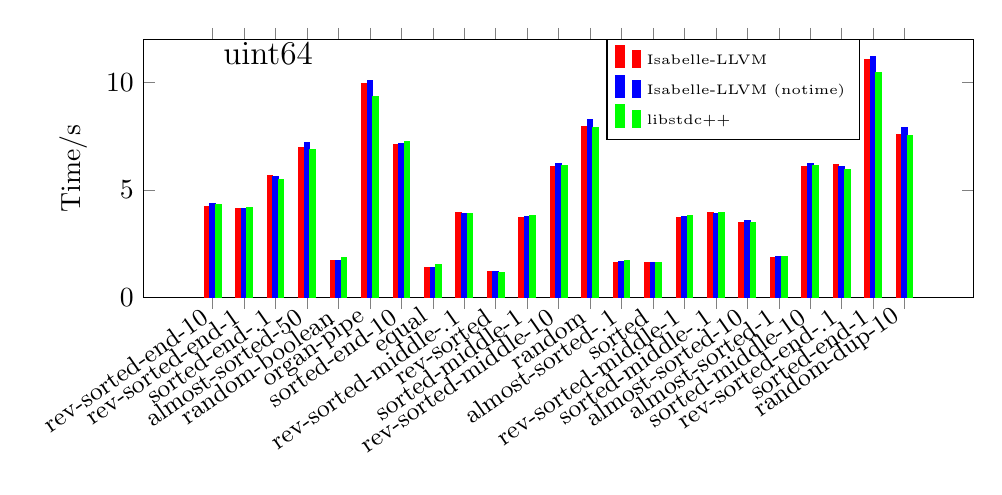
\begin{tikzpicture}
    \begin{axis}[
%       xlabel={Benchmark Set},
      xlabel near ticks,
      ylabel={Time/s},
      title={\large uint64},
      title style={at={(0.15,.80)}},
      scaled y ticks=manual:{}{
        \pgfmathparse{#1/1000}
        },      
      legend style = {
        at={(.71,.61)},
        anchor=south,
        cells={anchor=west},
        font=\tiny
      },
      ybar=0pt,
%      ymin=0,
%       ymax=1e4,
      width=\textwidth,
      height=\textwidth*0.4,
      bar width=2.0pt,
      symbolic x coords={rev-sorted-end-10,rev-sorted-end-1,sorted-end-.1,almost-sorted-50,random-boolean,organ-pipe,sorted-end-10,equal,rev-sorted-middle-.1,rev-sorted,sorted-middle-1,rev-sorted-middle-10,random,almost-sorted-.1,sorted,rev-sorted-middle-1,sorted-middle-.1,almost-sorted-10,almost-sorted-1,sorted-middle-10,rev-sorted-end-.1,sorted-end-1,random-dup-10,},      
      xtick=data,
%       nodes near coords,
%       nodes near coords align={vertical},
      x tick label style={rotate=35,anchor=east,font=\small},
%       ytick={1e3,1e4},
      ymin=0,
      ymax=1.2e4,
      restrict y to domain=0:1.2e4,
%       ytick distance = 10,
%       ytickten = {1,2,3,4,5},
    ]
            
        \addplot[color=red,fill=red] coordinates {
        (rev-sorted-end-10,4236)
        (rev-sorted-end-1,4126)
        (sorted-end-.1,5670)
        (almost-sorted-50,6987)
        (random-boolean,1699)
        (organ-pipe,9950)
        (sorted-end-10,7134)
        (equal,1388)
        (rev-sorted-middle-.1,3937)
        (rev-sorted,1201)
        (sorted-middle-1,3730)
        (rev-sorted-middle-10,6068)
        (random,7973)
        (almost-sorted-.1,1628)
        (sorted,1614)
        (rev-sorted-middle-1,3716)
        (sorted-middle-.1,3945)
        (almost-sorted-10,3481)
        (almost-sorted-1,1836)
        (sorted-middle-10,6076)
        (rev-sorted-end-.1,6192)
        (sorted-end-1,11100)
        (random-dup-10,7559)
        };
        \addlegendentry{Isabelle-LLVM};

        \addplot[color=blue,fill=blue] coordinates {
        (rev-sorted-end-10,4354)
        (rev-sorted-end-1,4120)
        (sorted-end-.1,5605)
        (almost-sorted-50,7225)
        (random-boolean,1699)
        (organ-pipe,10106)
        (sorted-end-10,7175)
        (equal,1379)
        (rev-sorted-middle-.1,3904)
        (rev-sorted,1199)
        (sorted-middle-1,3747)
        (rev-sorted-middle-10,6221)
        (random,8281)
        (almost-sorted-.1,1644)
        (sorted,1633)
        (rev-sorted-middle-1,3771)
        (sorted-middle-.1,3901)
        (almost-sorted-10,3554)
        (almost-sorted-1,1878)
        (sorted-middle-10,6237)
        (rev-sorted-end-.1,6106)
        (sorted-end-1,11218)
        (random-dup-10,7889)
        };
        \addlegendentry{Isabelle-LLVM (notime)};
        
        
        \addplot[color=green,fill=green] coordinates {
        (rev-sorted-end-10,4325)
        (rev-sorted-end-1,4174)
        (sorted-end-.1,5478)
        (almost-sorted-50,6900)
        (random-boolean,1830)
        (organ-pipe,9350)
        (sorted-end-10,7233)
        (equal,1503)
        (rev-sorted-middle-.1,3916)
        (rev-sorted,1148)
        (sorted-middle-1,3799)
        (rev-sorted-middle-10,6156)
        (random,7924)
        (almost-sorted-.1,1685)
        (sorted,1608)
        (rev-sorted-middle-1,3787)
        (sorted-middle-.1,3931)
        (almost-sorted-10,3490)
        (almost-sorted-1,1875)
        (sorted-middle-10,6146)
        (rev-sorted-end-.1,5933)
        (sorted-end-1,10476)
        (random-dup-10,7512)
        };
        \addlegendentry{libstdc++};


        
        
        % \addplot[color=black,fill=black] coordinates {
        % (rev-sorted-end-10,4252)
        % (rev-sorted-end-1,4205)
        % (sorted-end-.1,5520)
        % (almost-sorted-50,6807)
        % (random-boolean,1719)
        % (organ-pipe,10171)
        % (sorted-end-10,7211)
        % (equal,1373)
        % (rev-sorted-middle-.1,3901)
        % (rev-sorted,1129)
        % (sorted-middle-1,3769)
        % (rev-sorted-middle-10,6073)
        % (random,8011)
        % (almost-sorted-.1,1635)
        % (sorted,1608)
        % (rev-sorted-middle-1,3777)
        % (sorted-middle-.1,3907)
        % (almost-sorted-10,3287)
        % (almost-sorted-1,1880)
        % (sorted-middle-10,6085)
        % (rev-sorted-end-.1,6215)
        % (sorted-end-1,10944)
        % (random-dup-10,7644)
        % };
        % \addlegendentry{C++ (orig)};



    \end{axis}
  \end{tikzpicture}
  
  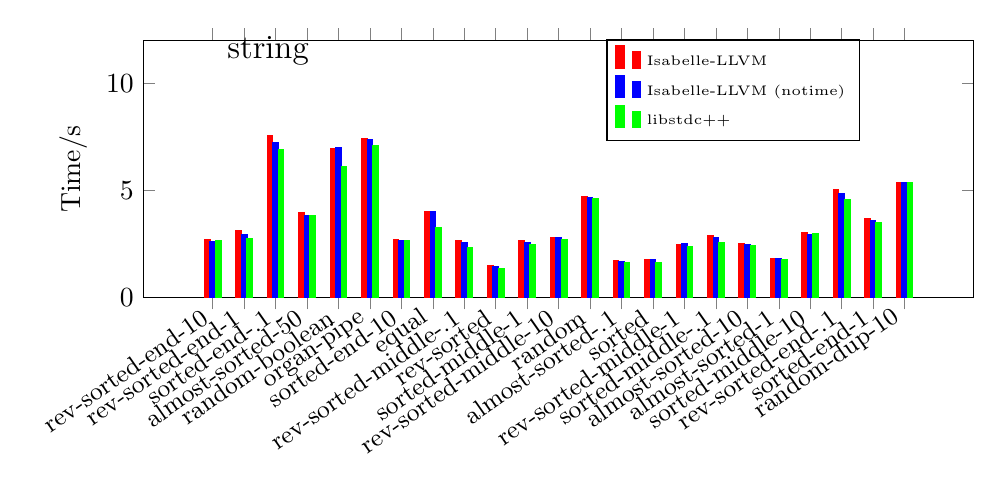
\begin{tikzpicture}
    \begin{axis}[
%       xlabel={Benchmark Set},
      xlabel near ticks,
      ylabel={Time/s},
      title={\large string},
      title style={at={(0.15,.80)}},
      scaled y ticks=manual:{}{
        \pgfmathparse{#1/1000}
        },      
      legend style = {
        at={(.71,.61)},
        anchor=south,
        cells={anchor=west},
        font=\tiny
      },
      ybar=0pt,
%      ymin=0,
%       ymax=1e4,
      width=\textwidth,
      height=\textwidth*0.4,
      bar width=2.0pt,
      symbolic x coords={rev-sorted-end-10,rev-sorted-end-1,sorted-end-.1,almost-sorted-50,random-boolean,organ-pipe,sorted-end-10,equal,rev-sorted-middle-.1,rev-sorted,sorted-middle-1,rev-sorted-middle-10,random,almost-sorted-.1,sorted,rev-sorted-middle-1,sorted-middle-.1,almost-sorted-10,almost-sorted-1,sorted-middle-10,rev-sorted-end-.1,sorted-end-1,random-dup-10,},      
      xtick=data,
%       nodes near coords,
%       nodes near coords align={vertical},
      x tick label style={rotate=35,anchor=east,font=\small},
%       ytick={1e3,1e4},
      ymin=0,
      ymax=1.2e4,
      restrict y to domain=0:1.2e4,
%       ytick distance = 10,
%       ytickten = {1,2,3,4,5},
    ]
            
\addplot[color=red,fill=red] coordinates {
(rev-sorted-end-10,2697)
(rev-sorted-end-1,3108)
(sorted-end-.1,7570)
(almost-sorted-50,3951)
(random-boolean,6965)
(organ-pipe,7439)
(sorted-end-10,2705)
(equal,4008)
(rev-sorted-middle-.1,2659)
(rev-sorted,1475)
(sorted-middle-1,2673)
(rev-sorted-middle-10,2783)
(random,4707)
(almost-sorted-.1,1717)
(sorted,1774)
(rev-sorted-middle-1,2486)
(sorted-middle-.1,2894)
(almost-sorted-10,2508)
(almost-sorted-1,1825)
(sorted-middle-10,3054)
(rev-sorted-end-.1,5055)
(sorted-end-1,3686)
(random-dup-10,5371)
};
\addlegendentry{Isabelle-LLVM};
\addplot[color=blue,fill=blue] coordinates {
(rev-sorted-end-10,2633)
(rev-sorted-end-1,2947)
(sorted-end-.1,7216)
(almost-sorted-50,3809)
(random-boolean,7004)
(organ-pipe,7372)
(sorted-end-10,2682)
(equal,4004)
(rev-sorted-middle-.1,2572)
(rev-sorted,1441)
(sorted-middle-1,2555)
(rev-sorted-middle-10,2798)
(random,4672)
(almost-sorted-.1,1698)
(sorted,1768)
(rev-sorted-middle-1,2517)
(sorted-middle-.1,2825)
(almost-sorted-10,2456)
(almost-sorted-1,1822)
(sorted-middle-10,2924)
(rev-sorted-end-.1,4872)
(sorted-end-1,3615)
(random-dup-10,5377)
};
\addlegendentry{Isabelle-LLVM (notime)};

\addplot[color=green,fill=green] coordinates {
(rev-sorted-end-10,2665)
(rev-sorted-end-1,2768)
(sorted-end-.1,6917)
(almost-sorted-50,3815)
(random-boolean,6114)
(organ-pipe,7079)
(sorted-end-10,2649)
(equal,3255)
(rev-sorted-middle-.1,2359)
(rev-sorted,1354)
(sorted-middle-1,2487)
(rev-sorted-middle-10,2700)
(random,4604)
(almost-sorted-.1,1647)
(sorted,1623)
(rev-sorted-middle-1,2402)
(sorted-middle-.1,2575)
(almost-sorted-10,2447)
(almost-sorted-1,1774)
(sorted-middle-10,3001)
(rev-sorted-end-.1,4566)
(sorted-end-1,3489)
(random-dup-10,5356)
};
\addlegendentry{libstdc++};


    \end{axis}
  \end{tikzpicture}
  
  \caption{Comparison of the running time measured for the code generated by the formalization described in this paper (Isabelle-LLVM), the original formalization from~\cite{Lammich20} (notime), and the \emph{libstdc++} implementation. 
  %
  Arrays with $10^8$ \is{uint64}s and $10^7$ \is{string}s with various distributions were sorted, and we display the smallest time of 10 runs. The programs were compiled with \emph{clang-10 -O3}, and run on an Intel XEON E5-2699 with 128GiB RAM and 256K/55M L2/L3 cache.
%   Arrays with $10^8$ \is{uint64}s with various distributions were sorted on an Intel XEON E5-2699 with 128GiB RAM, and 256K/55M L2/L3 cache. For compilation, we used clang-10 with optimization level O3. We averaged over 10 runs.
  }\label{fig:bench}
  \vspace{-1em}
\end{figure}




% - compiler: clang10 
% - flags:  -O3
% - number of runs you average over: 10
% - lxcisa0: 
%  -> Intel(R) Xeon(R) CPU E5-2699 v4 @ 2.20GHz
%  -> 128  GB RAM
%   -> lscpu gibt: (L1/2/3:32K/256K/56320K)

%     L1 cache:               32K

%     L2 cache:              256K 

%     L3 cache:              56320K



\section{Conclusions}\label{sec:conclusion}
We have presented a refinement framework for the simultaneous verification of functional correctness and complexity of algorithm implementations with competitive practical performance. 

We use stepwise refinement to separate high-level algorithmic ideas from low-level optimizations, enabling convenient verification of highly optimized algorithms. 
The novel concept of resource currencies allows structuring of the complexity proofs along the refinement chain. Refinement also works seamlessly for amortized data structures. 
Our framework refines down to the LLVM intermediate representation, such that we can use a state-of-the-art compiler to generate performant programs.

As a case study, we have proved the functional correctness and complexity of the introsort sorting algorithm. Our design supports arbitrary element types, even those with non-constant-time compare operations, like strings.
%
Our verified implementation performs on par with the (unverified) state-of-the-art implementation from the GNU C++ Library. It also provably meets the C++11 standard library~\cite{stdlib-sort} specification for \emph{std::sort}, which in particular requires a worst-case time complexity of \is{O($n \log n$)}.
%
We are not aware of any other verified implementations of real-world sorting algorithms that come with a complexity analysis.

% The fine-grained analysis of operation counts Musser~\cite[Table 1]{Musser97} conducts only empirically can now be performed with a verified worst-case analysis. 
%Our result additionally allows a fine-grained worst-case analysis of operation counts, which Musser~\cite[Table 1]{Musser97} only conducted empirically.

Our work is a combination and substantial extension of an earlier refinement framework for functional correctness~\cite{lammich2019LLVM} which also comes with a verification of introsort~\cite{Lammich20}, and a refinement framework for a single \emph{enat}-valued currency \cite{HaslbeckL19}.
In particular, we have generalized the refinement framework to arbitrary resources, applied it to amortized analysis,
introduced currencies that help organizing refinement proofs, extended the LLVM semantics and reasoning infrastructure with a cost model, connected it to the refinement framework via a new version of the Sepref tool, and, finally, added the complexity analysis for introsort.

% In the process we generalized the NREST-monad to arbitrary resources, extended the LLVM semantics with a cost model and connected the two with a new version of the Sepref tool.


\subsection{Related Work}



% - other sorting algorithm verifications
%   - maybe even with running time analysis
% - where does the idea to generalize nres come from?
% - why the connection to "a fistful of dollars"

%\paragraph{Sorting algorithms}

Nipkow \emph{et al.}~\cite[\S 4.1]{NipkowEH-ATVA20} collect verification efforts concerning sorting algorithms.
%, from theoretical results to industrial applications.
We add a few instances verifying running time:
%Eberl \cite{Comparison_Sort_Lower_Bound-AFP} proves the well known lower bound $\Omega(n \log n)$ for comparison based sorting algorithms.
%Van der Weegen and McKinna~\cite{WeegenM08} (Coq) an Eberl~\cite{Quick_Sort_Cost-AFP,EberlHN20} (Isabelle) prove the correctness and expected running time of randomized quicksort as well as average-case running time of deterministic quicksort.
%De Gou et al.~\cite{GouwBBHRS19} verify timsort's termination and exception freedom using KeY. % JAR 2019
%Beckert et al.~\cite{BeckertSSU17} verify the dual-pivot quicksort algorithm from the Java standard library.
%
% Atkey~\cite{Atkey11} analyzed the running time of the merge operation in mergesort: the number of comparisons linear in the length of the list
Wang \emph{et al.} use TiML~\cite{WangWC17} to verify correctness and asymptotic time complexity of mergesort automatically.
Zhan and Haslbeck \cite{zhan2018verifying} verify functional correctness and asymptotic running time analysis of imperative versions of insertion sort and mergesort.
% (AARA) Expected running time analysis of probabilistic algorithms \cite{WangKH20}
We build on earlier work by Lammich~\cite{Lammich20} and provide the first verification of functional correctness and asymptotic running time analysis of heapsort and introsort.

The following are the most complex algorithms and data structures with verified running time analysis using time credits and separation logic we are aware of:
a linear time selection algorithm \cite{zhan2018verifying}, an incremental cycle detection algorithm \cite{gueneau-chargueraud-jourdan-pottier-19}, Union-Find \cite{ChargueraudP19}, Edmonds-Karp and Kruskal's algorithm \cite{HaslbeckL19}.

%\paragraph{Quantitative algorithm analysis}

% Carbonneaux et al. \cite{Carbonneaux0RS14} use potential functions (\is{state -> enat}) instead of predicates (\is{state -> bool}), present a quantitative Hoare logic and extend the CompCert compiler to preserve properties of stack-usage from programs in Clight to compiled programs. % "quantitative CompCert"

% Their lifting idea lead us to generalize the nres monad by Lammich \cite{lammich2012applying,lammich2013automatic,refinement} (essentially NREST with \is{$\gamma$=unit}) first to extended natural numbers \cite{HaslbeckL19} and now to arbitrary resources \is{$\gamma$}.

The idea to generalize the nres monad~\cite{lammich2012applying} to resource types originates from Carbonneaux \emph{et al.} \cite{Carbonneaux0RS14}.
They use potential functions (\is{state -> enat}) instead of predicates (\is{state -> bool}), present a quantitative Hoare logic, and extend the CompCert compiler to preserve properties of stack-usage from programs in Clight to compiled programs.
Observe, that the step from qualitative \cite{Dijkstra76} to quantitative weakest preconditions (\cf\ Section~\ref{sec:refinement_patterns}) is similar to the weakest preexpectation transformer by Kozen \cite{Kozen85}, and the expected running time transformer \is{ert} by Kaminski \etAl\ \cite{kaminski2016weakest}.

Rajani \etAl~\cite{RajaniG0021} present a unifying type-theory \is{$\lambda^{amor}$} for higher-order amortized cost analysis, which involves a cost monad similar to NREST without nondeterminism.
The introduction of the \is{elapse} combinator is straightforward, but the \is{reclaim} operator in NREST seems to be related to their type constructor \is{[p]$\tau$}. That constructor is central to their paper.
Rajani \cite{DRajani20} applies type-theoretic approach to Information Flow Control and generalizes the theory to allow any commutative monoid in the cost monad.
It would be interesting to see whether their cost monad can be extended to nondeterminism.
%\paragraph{Time credit separation logics}

We see our paper in the line of research concerning simultaneously verifying functional correctness and worst-case time complexity of algorithms.
Atkey~\cite{Atkey10} pioneered resource analysis with separation logic.
Chargu\'{e}raud and Pottier \cite{ChargueraudP15,ChargueraudP19} present a framework that uses time credits in Coq and apply it to the Union-Find data structure.
Gu\'{e}neau \emph{et al.} extend that framework with big-O style specifications \cite{fistful} and possibly negative time credits, and apply it to involved algorithms and data structures \cite{gueneau-chargueraud-jourdan-pottier-19}.
We further develop their work in three ways:
First, while time credits usually are natural numbers \cite{Atkey10,fistful,zhan2018verifying,MevelJP19,ChargueraudP19} or integers \cite{gueneau-chargueraud-jourdan-pottier-19},
we generalize to an abstract resource type and specifically use resource currencies for a fine-grained analysis.
Second, we use stepwise refinement to structure the verification and make the resource analysis of larger use-cases manageable.
Third, we provide facilities to automatically extract efficient competitive code from the verification.



% They all only produce code in functional or hybrid languages (OCaml, SML with mutable arrays).


% %mention Quantitative Separation logics?


% \paragraph{Other program semantics with resource usage}


% Carbonneaux et al. \cite{Carbonneaux0RS14} Stack-size for CompCert.

% Does Fiat \cite{DelawarePGC15} have something with time?



\subsection{Future Work}

% A next step to bring techniques of the verification community to industrial use in standard library would be to find further foundational algorithms that are suitable.

A verified compiler down to machine code would further reduce the trusted code base of our approach.
While that is not expected to be available soon for LLVM in Isabelle, the NREST-monad and the Sepref tool are general enough to connect to a different back end.
Formalizing one of the CompCert C semantics~\cite{BlazyL09} in Isabelle, connecting it to the NREST-monad and then processing synthesized C code with CompCert's verified compiler would be a way to go.

% The NREST-monad models abstract algorithms and their time consumption.
% It can be used to verify polynomial-time reductions and together with the Cook–Levin theorem prove NP-completeness of problems on an abstract level.
% The latter theorem needs to prove correctness and polynomial time of some algorithms on Turing machines. 
% Turing machines could be connected to NREST as another computational model, and the reasoning could be conducted on the abstract level, with finally synthesizing Turing machines automatically.

In this paper we apply our framework to verify an involved algorithm that only uses basic data structures, i.e.\ arrays.
A next step is to verify more involved data structures, e.g.\ by porting existing verifications of the Imperative Collections Framework~\cite{Lammich19_JAR} to LLVM.
We do not yet see how to reason about the running time of data structures like hash maps, where worst-case analysis would be possible but not useful.
In general, extending the framework to average-case analysis and probabilistic programs are exciting roads to take.

We plan to implement more automation, saving the user from writing boilerplate code when handling resource currencies and exchange rates.


Neither the LLVM nor the NREST level of our framework is 
tied to running time. 
Applying it to other resources like maximum heap space consumption might be a next step.




%%
%% The acknowledgments section is defined using the "acks" environment
%% (and NOT an unnumbered section). This ensures the proper
%% identification of the section in the article metadata, and the
%% consistent spelling of the heading.
\begin{acks}
% actually Gueneau read our ESOP draft and provided feedback 15.10.
% we talked about our work shortly before (?) the ESOP deadline (during POPL) with chargueraud and Pottier
We thank Arma{\"{e}}l Gu{\'{e}}neau, Arthur Chargu\'{e}raud, Fran{\c{c}}ois Pottier, and the anonymous referees of ESOP2021 and TOPLAS who provided valuable feedback on the earlier versions of this paper.
% This work was supported by the DFG Koselleck grant NI 491/16-1 ``Verifizierte Algorithmenanalyse'' and the DFG grant LA 3292/1 ``Verifizierte Model Checker''.
%
%Maximilian Haslbeck was supported by DFG Koselleck grant NI 491/16-1.
%Peter Lammich was supported by DFG Grant LA 3292/1 ``Verifizierte Model Checker''.
\end{acks}

%%
%% The next two lines define the bibliography style to be used, and
%% the bibliography file.
\bibliographystyle{ACM-Reference-Format}
\bibliography{paper}


\end{document}
\endinput
%%
%% End of file `sample-acmsmall.tex'.
